\cleardoublepage%
\chapter{\label{chap:res}Results and Discussion}%

%This is where you present your findings. As much as possible, structure your results along the lines of your research questions. Start with the simplest results first and proceed to more complex ones. Tables and Figures should be clear enough that they need little explanation: do not simply re-write the numbers as text to fill space. Rather, highlight trends, outliers, or gaps. 

\section{\label{sec:res_networking}Networking}%should this be in firmware?

As outlined in Section \ref{sec:methods_net_des} and Section \ref{sec:methods_net_dev}, and in accordance with research question 1, a networking structure has been conceptualised and implemented for use with the Smart Motors-based hardware.

\subsection{\label{sec:res_logic}Concept, Structure and Logic}

As outlined in Section \ref{sec:methods_net_des} and Section \ref{sec:methods_net_dev}, the networking was designed and developed in two parts: the Networking Library and, using this library as a base, the SSP Add-on Library. \\

The Networking library has been designed to serve as a general-purpose library, building upon ESP-NOW while incorporating essential structural and functional elements. It introduces address book logic that bypasses ESP-NOW's 20 peer limit, allowing transmission to a theoretically unlimited number of peers, though at the expense of efficiency. The library also introduces the fundamental message structure, including various message types (\textit{cmd}, \textit{inf}, \textit{ack}) and different subtypes (\textit{cmd}: \textit{ping}, \textit{echo}, \textit{boop}; \textit{inf}: \textit{msg}, \textit{data}; \textit{ack}: \textit{pong}, \textit{echo}, \textit{boop}, \textit{confirm}, \textit{success}, \textit{fail}). The library also includes logic to send data larger than $241\ bytes$, the maximum possible payload per message using the message structure defined in Section \ref{sec:rev_net}. This was increased to a theoretical limit of $60'928\ bytes$. In reality, however, the practical limit is lower, with the maximum amount successfully transmitted being about $30\ kB$ due to the memory limitations of the MicroPython firmware running on the ESP32C3. Additionally, the transmission of large messages in chunks entails the risk of some chunks being lost during transmission (see Section \ref{sec:res_rssi}), especially over long distances, resulting in the entire message being dropped. The code includes a provision to remedy this issue through the use of a buffer, wherein all components of a long message are stored. In the event that the receiving device fails to receive one or more parts of a multi-part message after a certain duration, it initiates a request for the missing parts. However, this functionality has been disabled to optimise memory usage. The network design incorporates a range of interfaces for customisation, with the potential for the inclusion of additional custom commands, message types and handling logic, including custom IRQ messages. \\

The SSP Add-on Library has been developed as an extension of the base Networking Library, introducing a range of additional Smart Module-specific commands, handlers and message types. These enable the effective control and configuration of Smart Modules through the utilisation of designated commands. The architecture of the code for both libraries, along with the full suite of commands available in each, is illustrated in Figure \ref{fig:net_code_structure}.\\

% \begin{figure}[H]
%     \centering
%     
\includegraphics[width=.5\linewidth]{overleaf/images/placeholder.png}
%     \vspace{\ftspace}
%     \caption{Networking overview}
%     \label{fig:Networking overview}
% \end{figure}

As such, the Networking Library fulfils the requirements outlined in Section \ref{sec:methods_net_des}. Notably, it is compatible with the Smart Motors hardware and with any ESP32-based hardware that includes Wi-Fi and thus ESP-NOW capabilities, as well as with the MicroPython firmware used. The protocol uses a peer-to-peer communication approach, inherited from ESP-NOW protocol, on which it is based, and requires no central root or hub, nor any configuration to use, other than initialising the library. The library also includes message validation features, employing a common message structure that includes an identifier and checksum. It further facilitates module discovery, using the \textit{ping} command, and interaction via various further defined commands and message types specified in Networking Library and the SSP Add-on Library, thereby satisfying the latter two requirements. In terms of design principles, the networking is split into two parts, allowing the base networking, which contains simple logic and commands, to be used in a variety of custom ways, further facilitated by interfaces for customisation. Finally, the code adheres to the Style Guide for Python Code based PEP 8 \citep{rossum_python_2001}.

\subsection{\label{sec:res_range}Maximum Range Test}

As described in Section \ref{sec:methods_test_range}, the original range test was conducted using the \textit{boop-o-meter} program on a street near the CEEO offices. The maximum range at which some messages were still being received by each of the two ESP32C3 MCBs was approximately 242 meters, as shown in Figure \ref{sec:res_range}, as measured using Google Earth.

\begin{figure}[H]
    \centering
    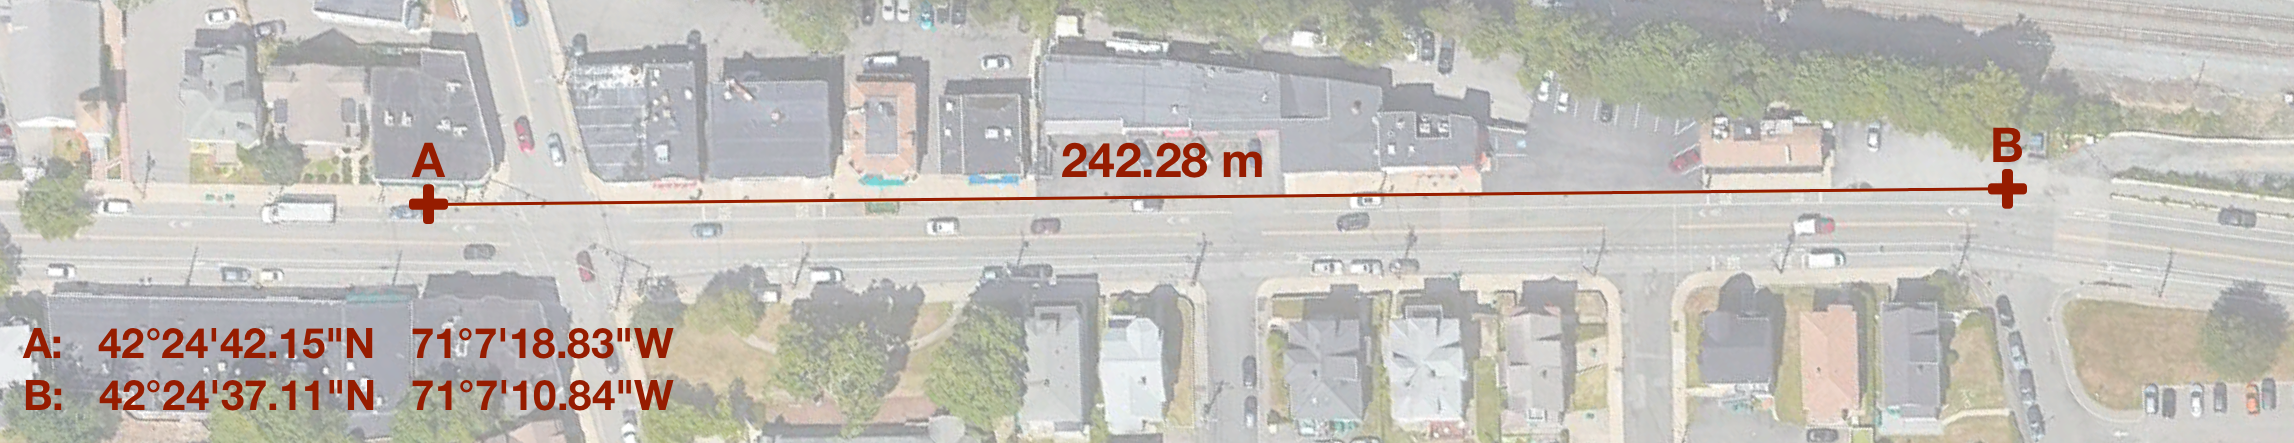
\includegraphics[width=\linewidth]{overleaf/images/range2.png}
    \vspace{.5\ftspace}
    \caption{Approximate maximum range test on Boston Avenue, MA}
    \label{fig:range}
\end{figure}


\subsection{\label{sec:res_rssi}Response Time, RSSI and Packet Loss Rate by Range}

The RSSI, ping response and packet loss for various ranges were measured three times using two ESP32C3s, one ESP32C3 and one ESP32C6 and again using two ESP32C6s.

\subsubsection{ESP32C3 to ESP32C3}

As anticipated, RSSI values, an index of signal strength, decrease for extended ranges, following a logarithmic curve, as shown in Figure \ref{sec:res_rssi}. The values for both devices are similar and follow a similar curve, with marginal divergence, likely attributed to material variations.

\begin{figure}[ht]
    \centering
    \begin{subfigure}{0.45\textwidth}
        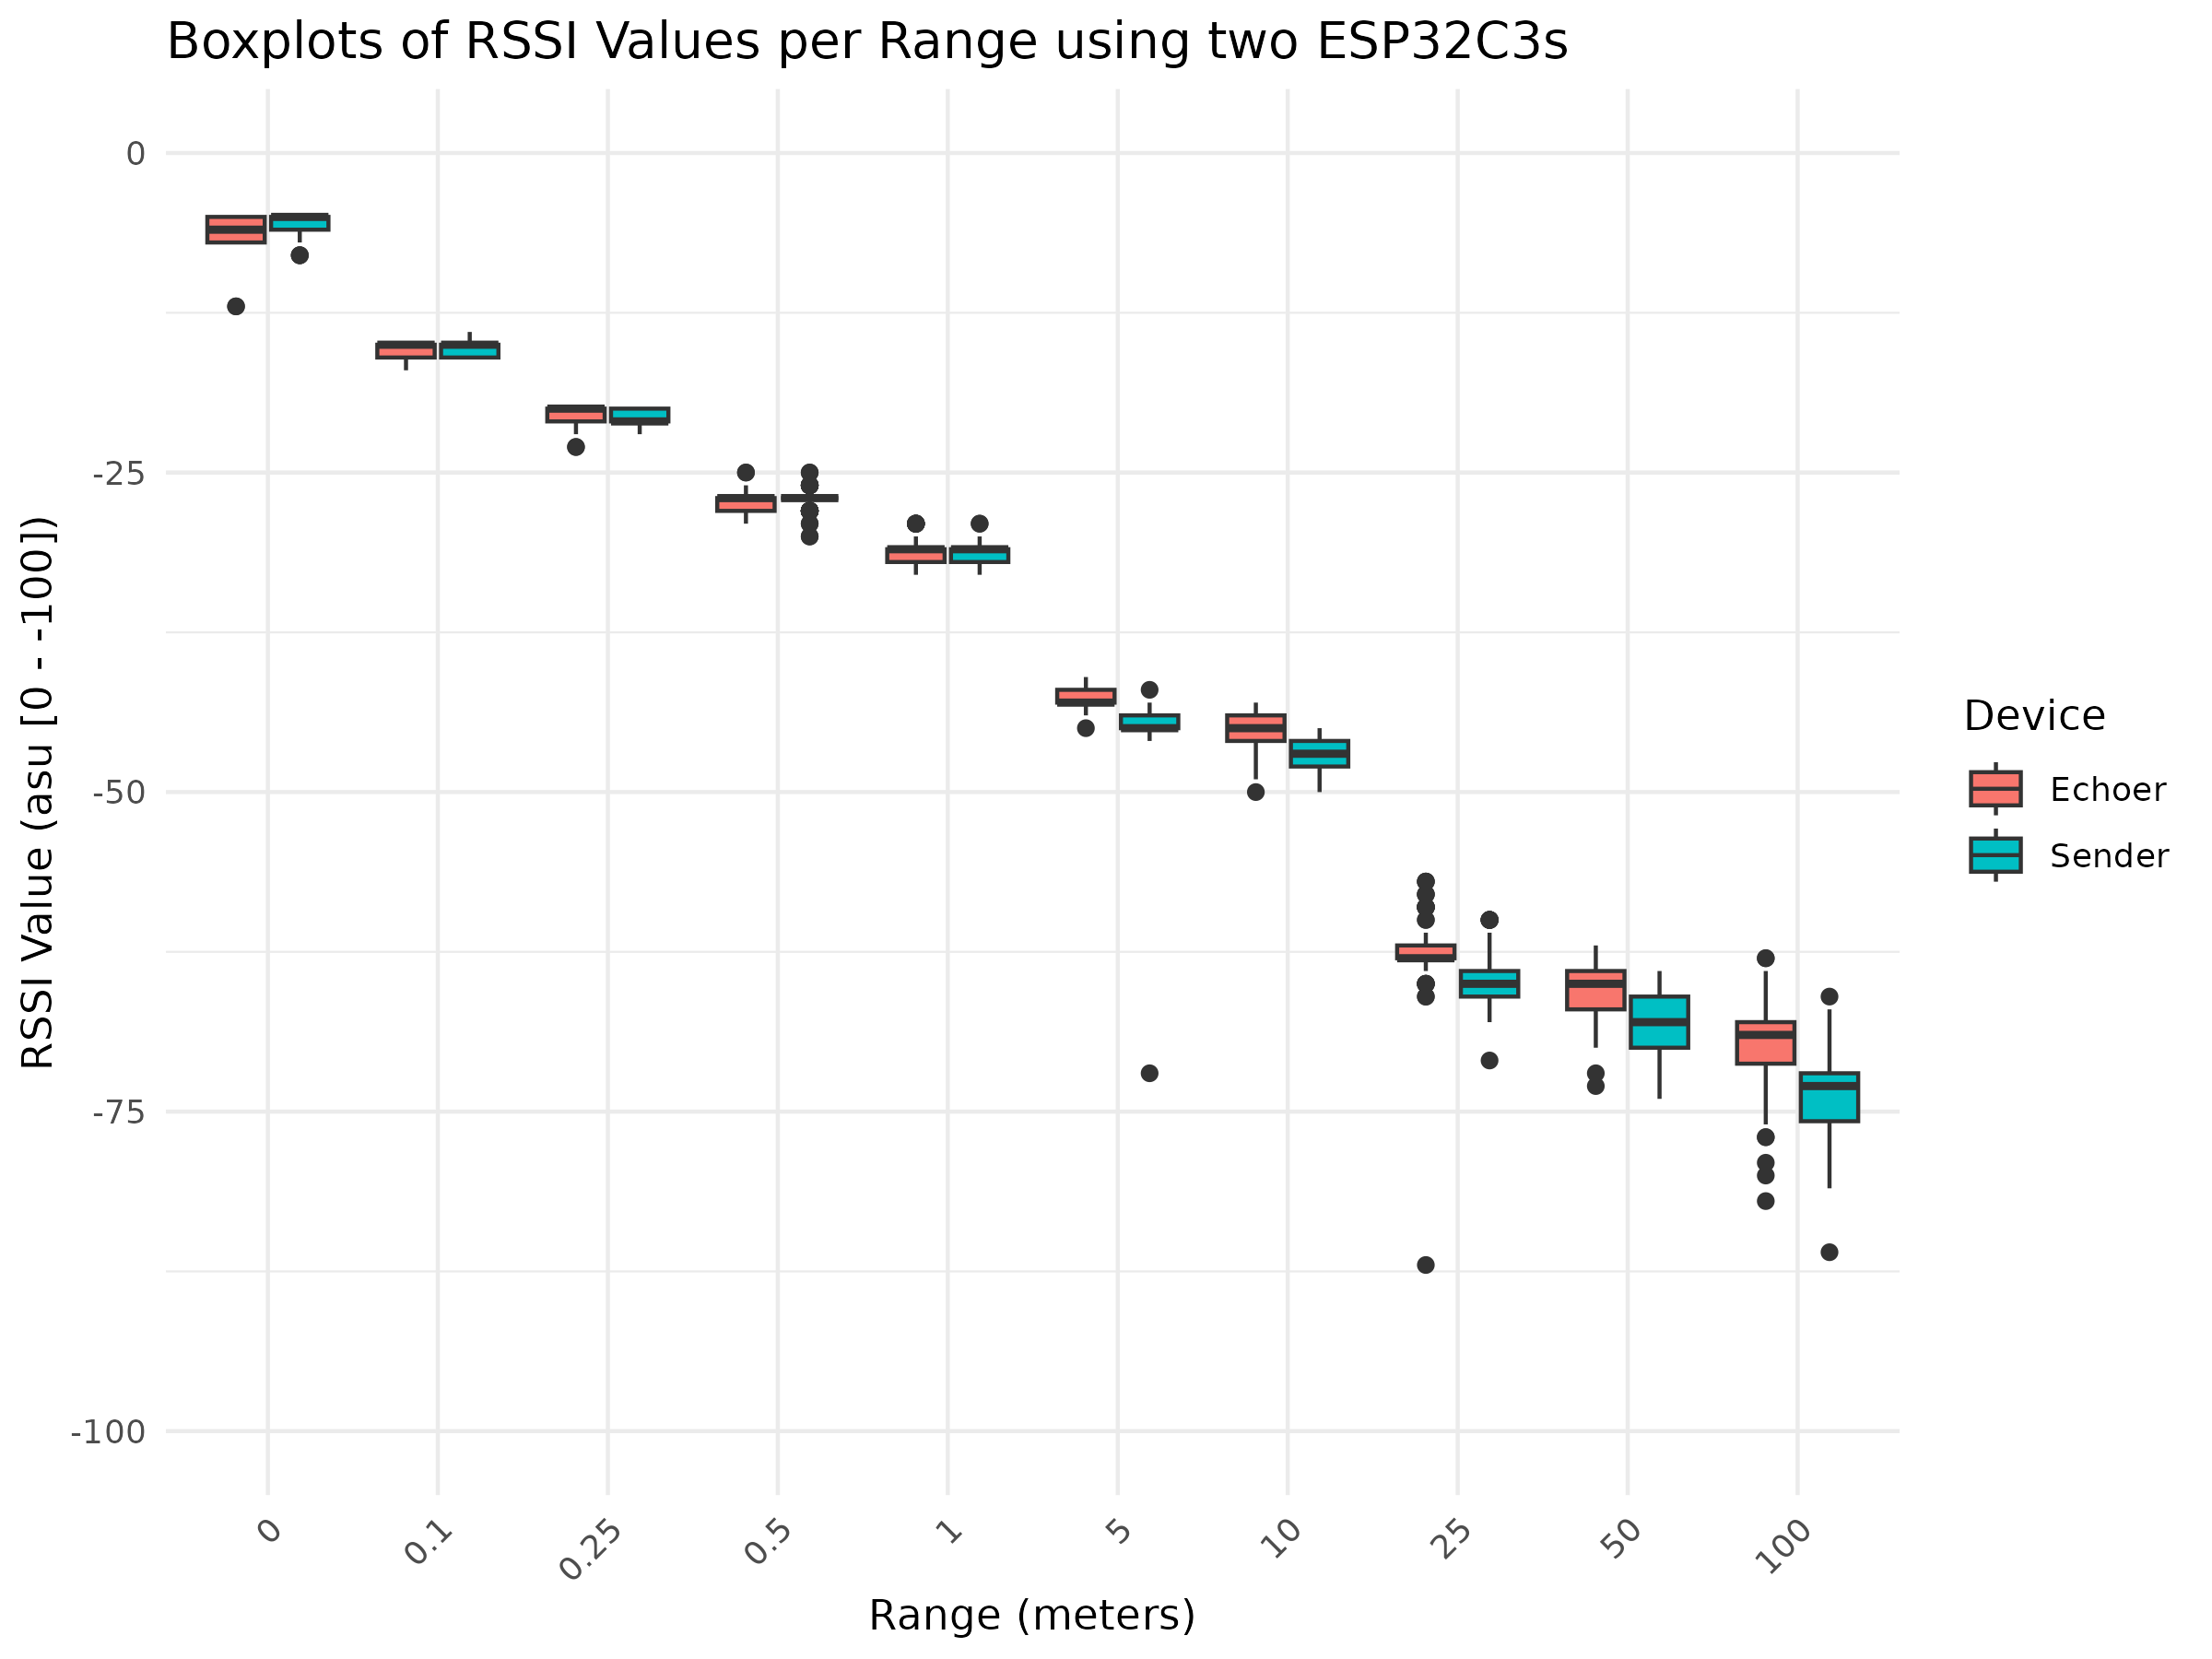
\includegraphics[width=\linewidth]{rstudio/analysis/plots/ESP32C3_rssi_box.png}
    \end{subfigure}
    \begin{subfigure}{0.45\textwidth}
        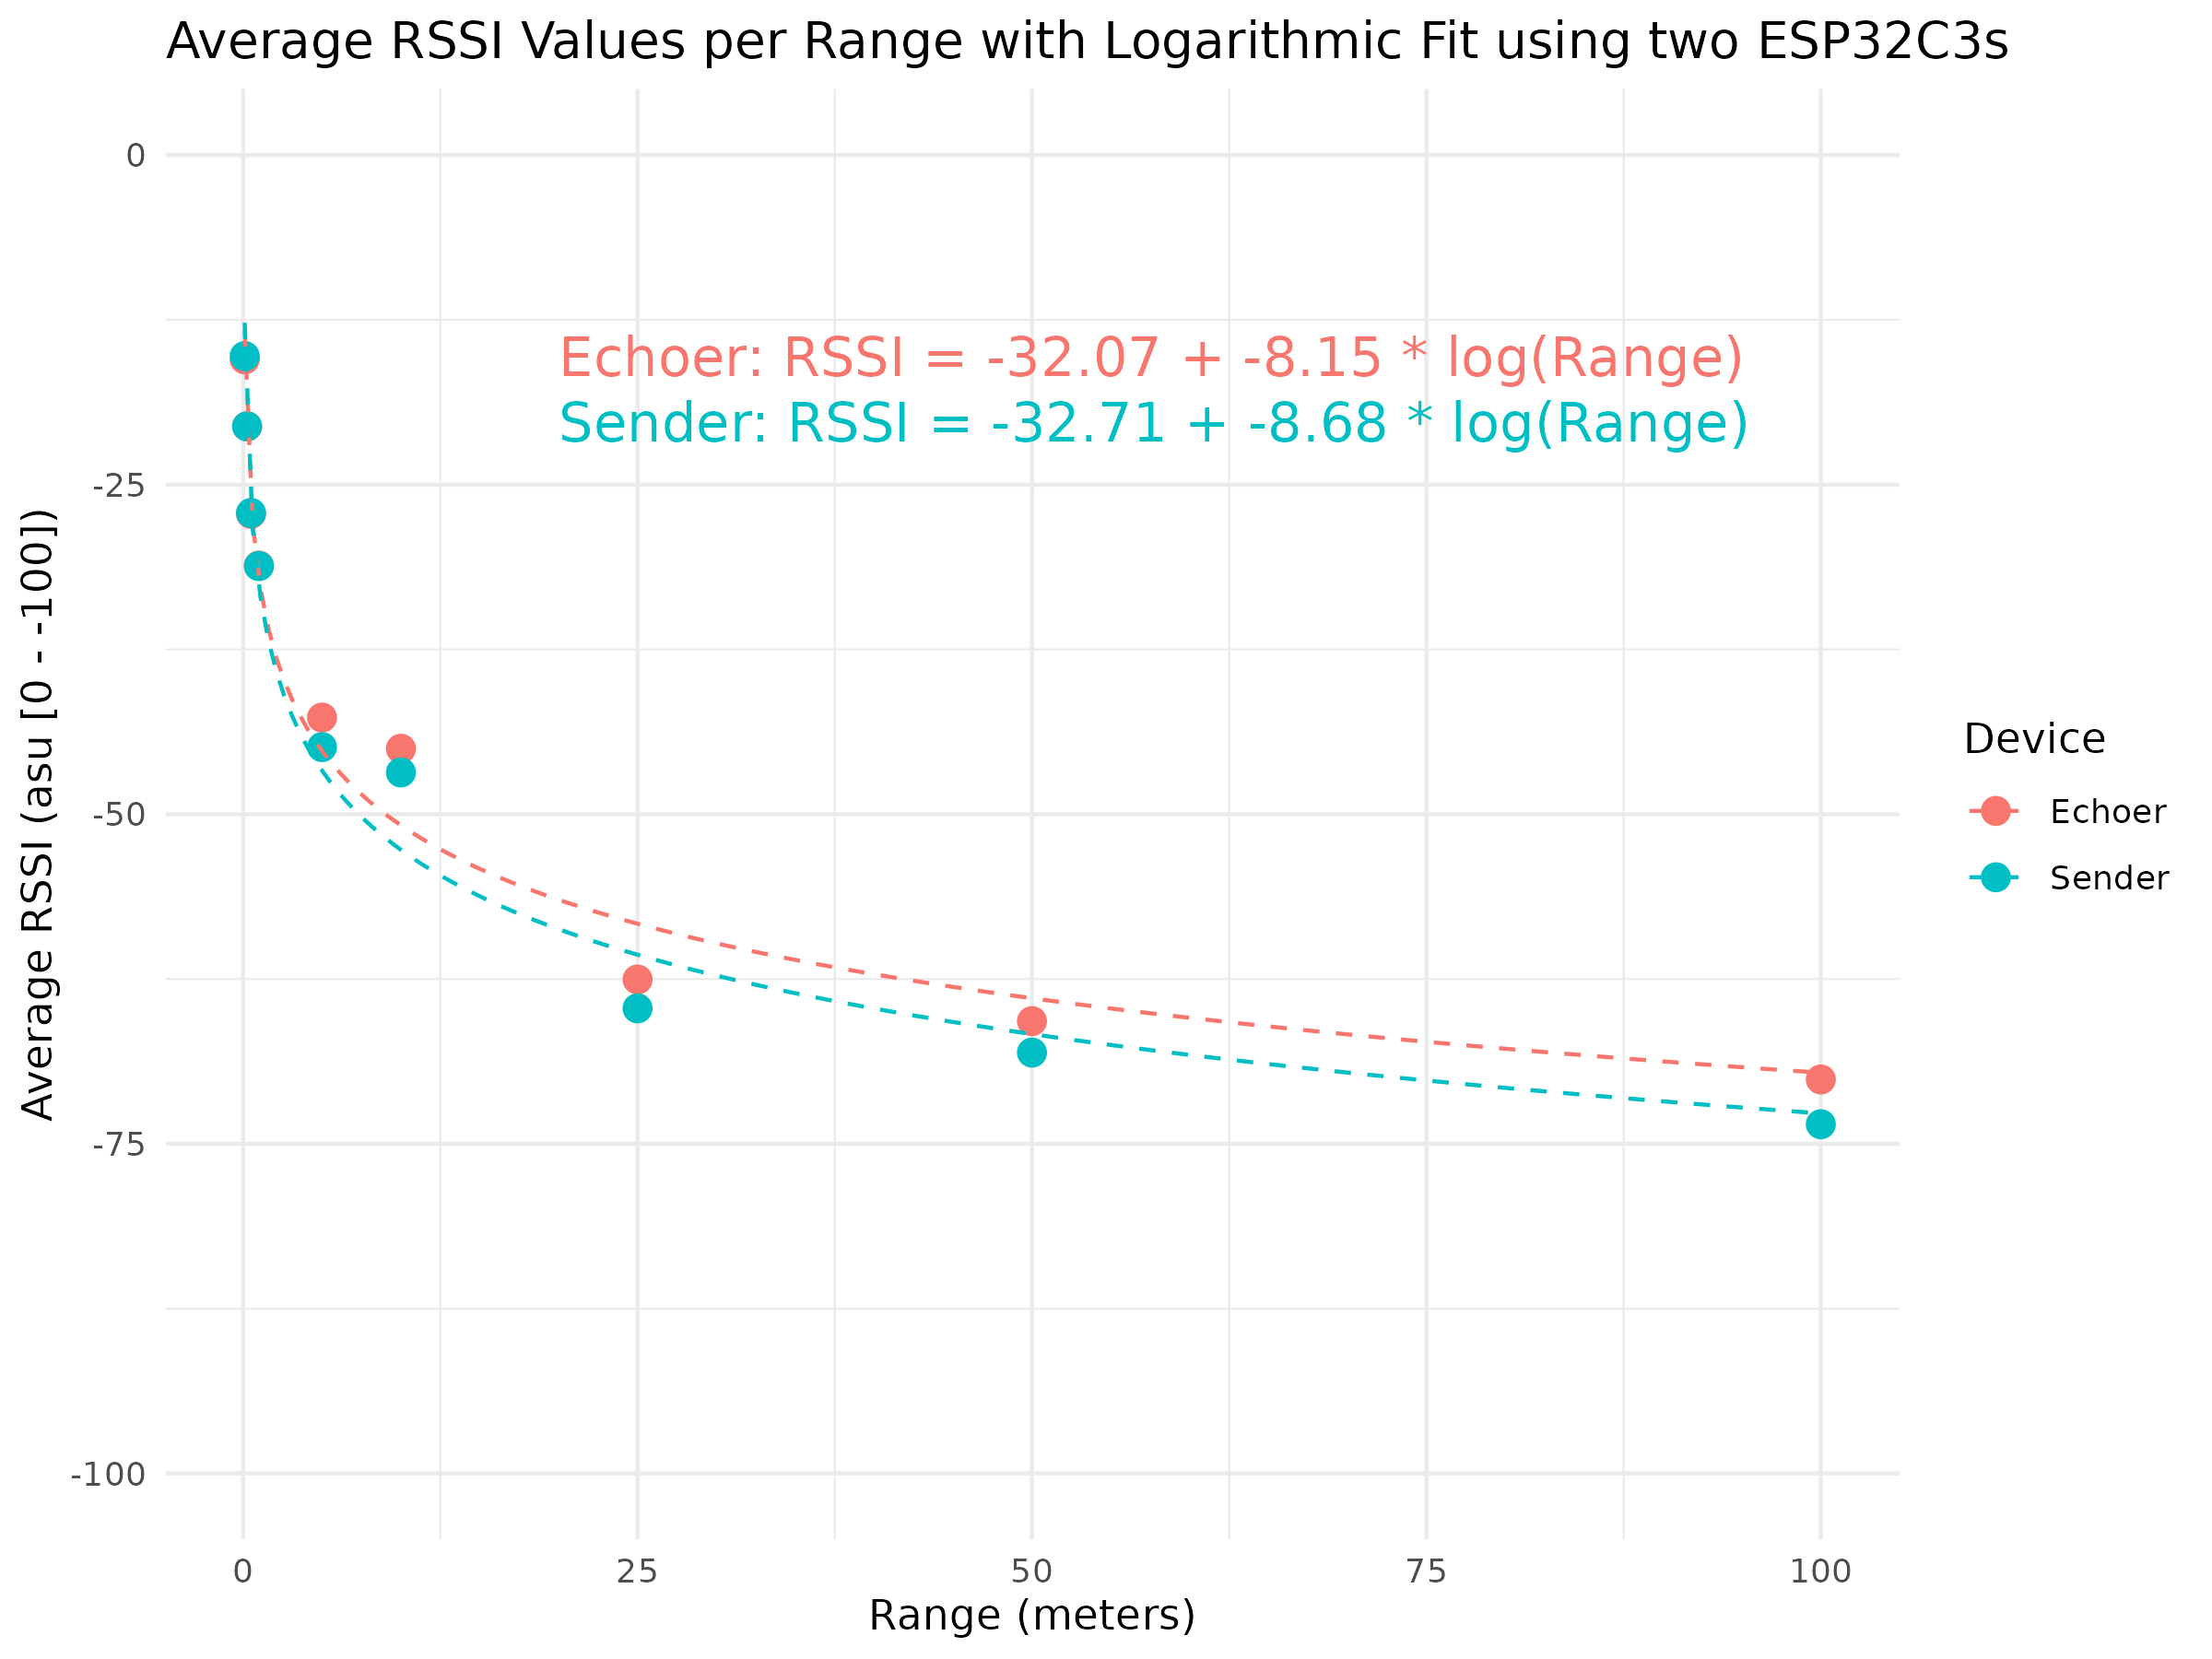
\includegraphics[width=\linewidth]{rstudio/analysis/plots/ESP32C3_avg_rssi.png}
    \end{subfigure}

    \begin{subfigure}{0.45\textwidth}
        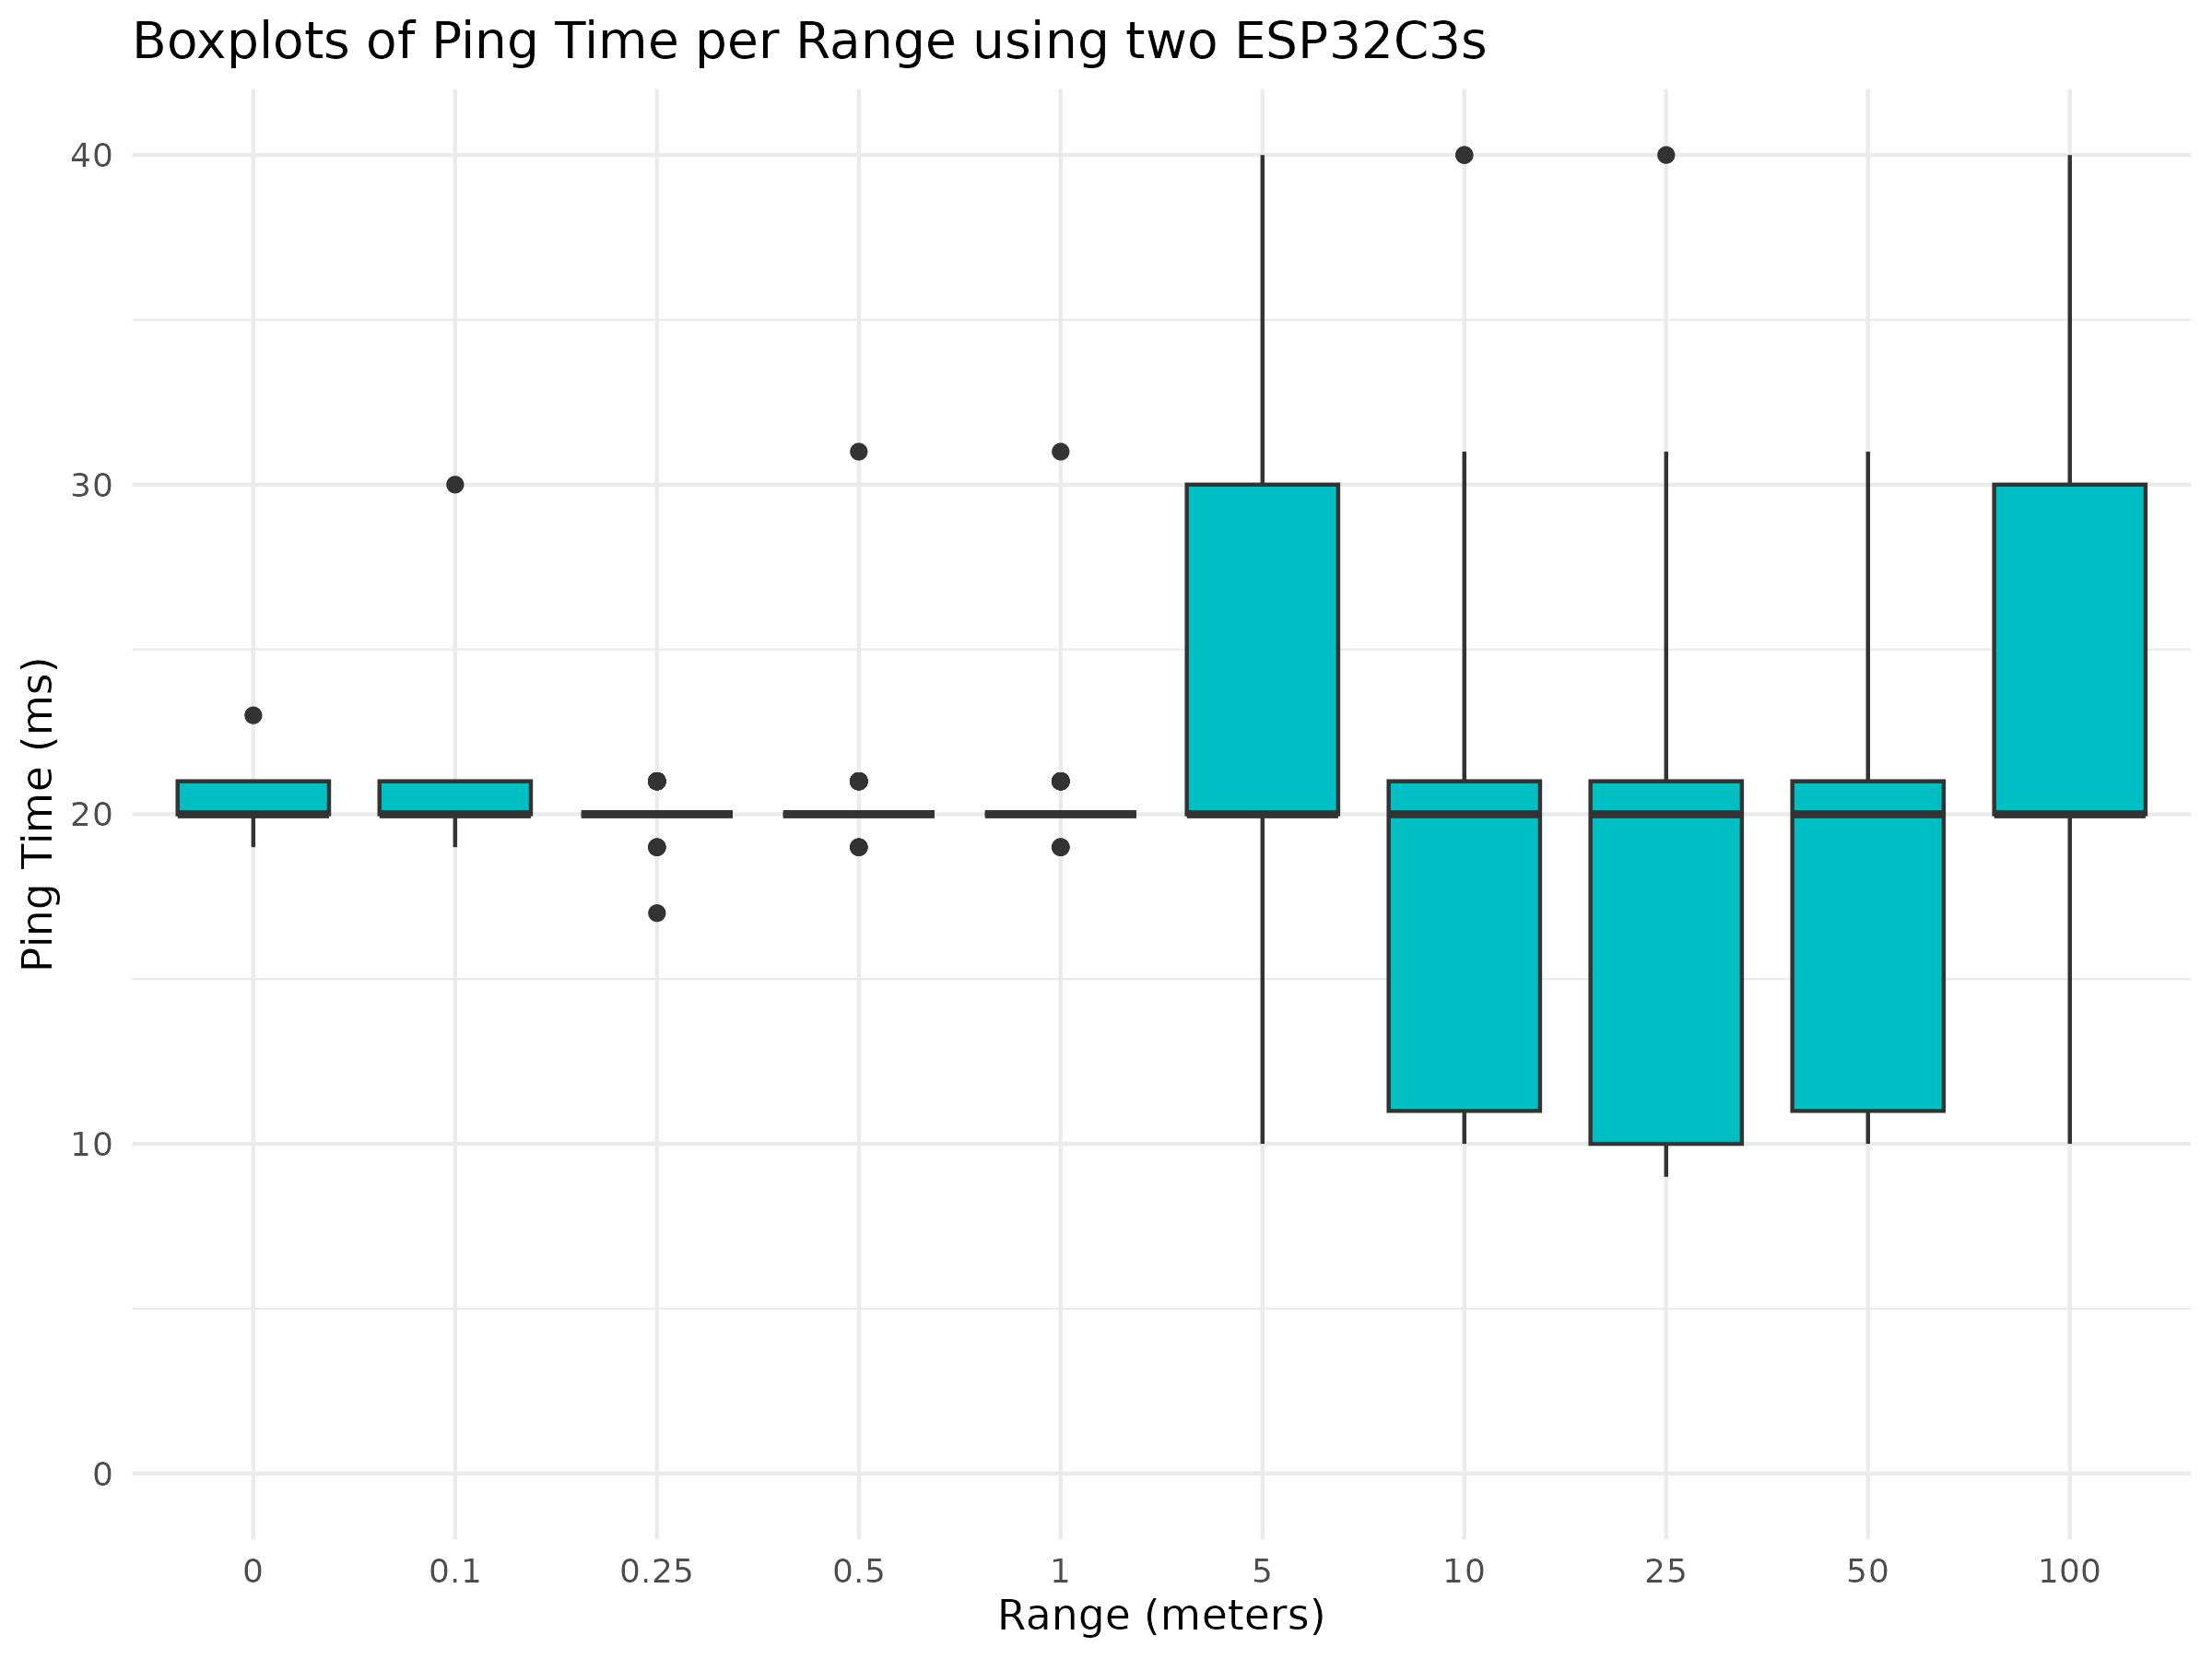
\includegraphics[width=\linewidth]{rstudio/analysis/plots/ESP32C3_ping_box.png}
    \end{subfigure}
    \begin{subfigure}{0.45\textwidth}
        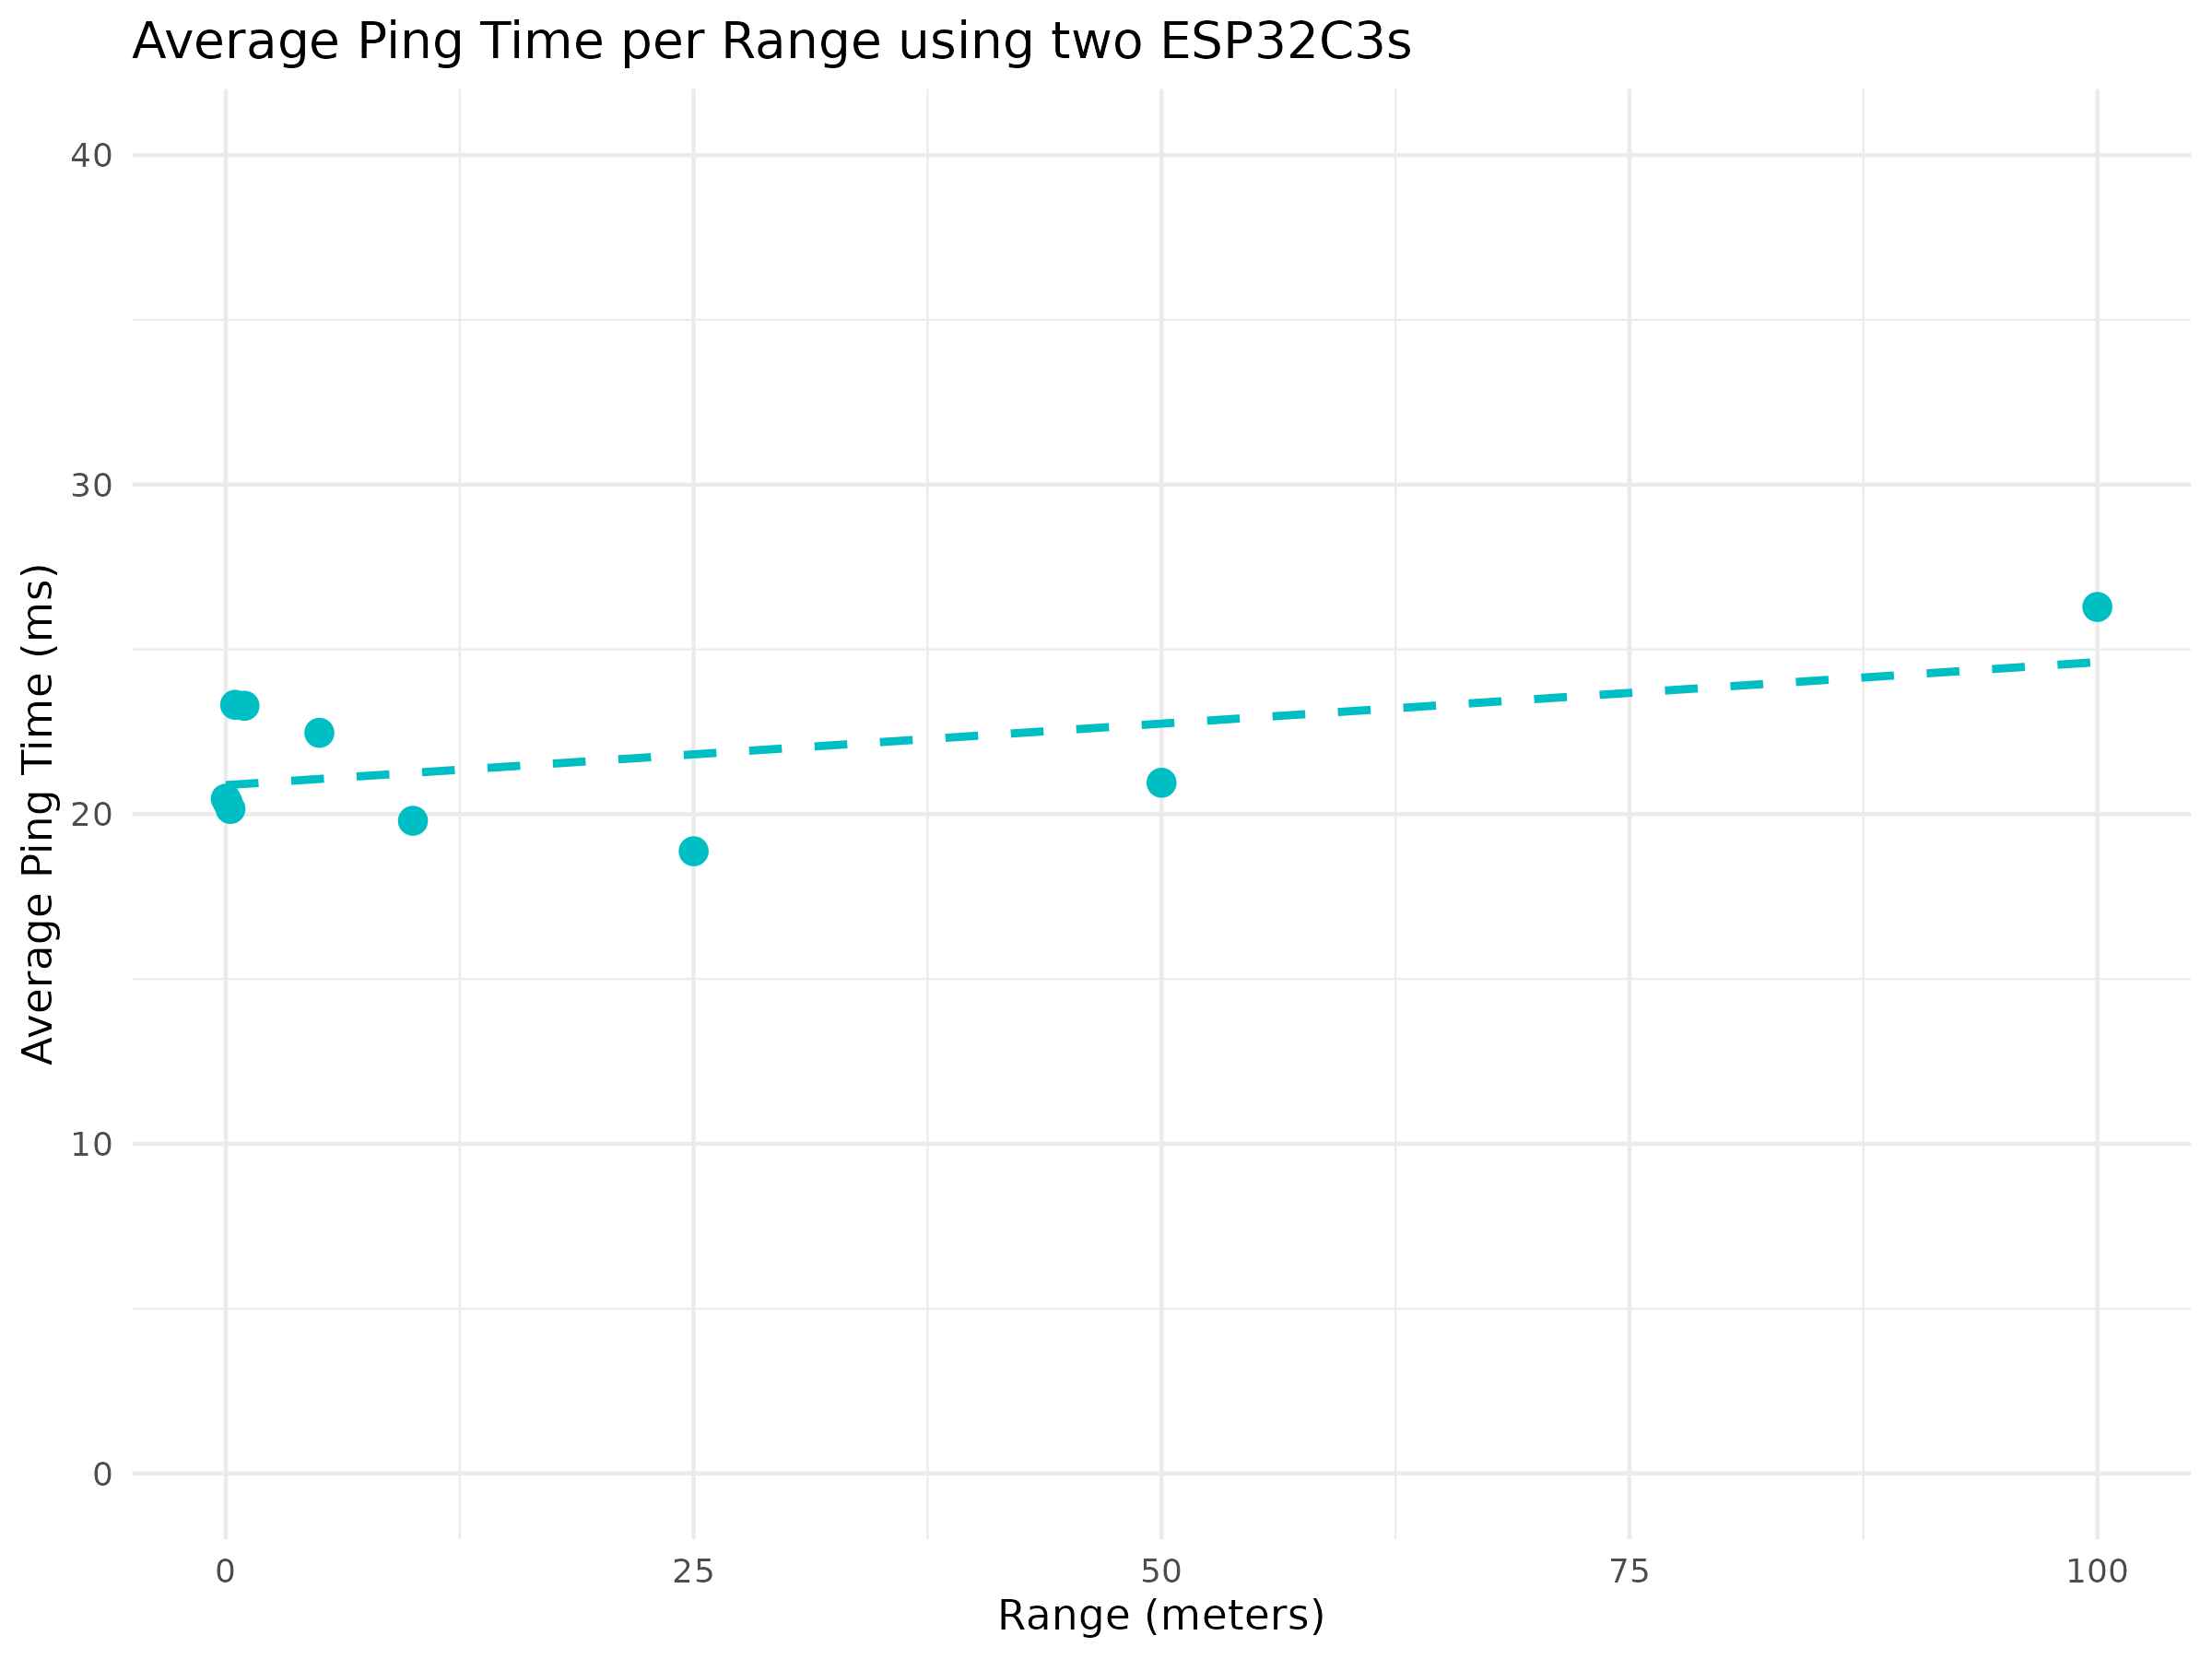
\includegraphics[width=\linewidth]{rstudio/analysis/plots/ESP32C3_avg_ping.png}
    \end{subfigure}
    \vspace{\ftspace}
    \caption{RSSI and ping response time depending on range using two ESP32C3s}
    \label{fig:rssipingrange_esp32c3}
\end{figure}

With regard to ping time, values remain largely unaffected by range, with a consistent median value of $20\ ms$ and mean values consistently around $20\ ms$. The increase in travel time from 0 to 100 meters of the radio wave is only approximately $0.0000033356\ ms$ ($100\ m\ /\ 299'792'458'000\ m/ms$), given the travel at the speed of light, which is insignificant compared to the time required to send and process the message by the MCB. Of particular interest is the observation that values are clustered at specific intervals of $10\ ms$, $20\ ms$, and $30\ ms$, which may be attributable to an underlying system clock rate of the MCB.

\begin{table}[H]
    \centering
    \begin{tabular}{|c|c|l|l|c|c|c|c|c|}
    \hline
        Range & Packet Loss & \multicolumn{2}{l|}{Measurement} & \multicolumn{5}{c|}{Values} \\\hline
        [meters] & [\%] & \multicolumn{2}{l|}{} & mean & std & min & max & median \\\hline\hline
        \multirow{3}{*}{0 m} & \multirow{1}{*}{0} & RSSI 1 & [asu] & -6.05 & 1.14 & -12 & -5 & -6 \\\cline{2-9}\cline{2-9}
        %&& Time 1 &  &  &  &  &  \\\cline{2-9}\cline{2-9}
        & \multirow{2}{*}{0} & RSSI 2 & [asu] & -5.44 & 0.67 & -8 & -5 & -5 \\\cline{3-9}
        %&& Time 2 &  &  &  &  &  \\\cline{3-9}
        && Ping & [ms] & 20.57 & 0.61 & 19 & 23 & 20 \\\hline\hline
        \multirow{3}{*}{0.1 m} & \multirow{1}{*}{0} & RSSI 1 & [asu] & -15.5 & 0.59 & -17 & -15 & -15 \\\cline{2-9}\cline{2-9}
        %&& Time 1 &  &  &  &  &  \\\cline{2-9}\cline{2-9}
        & \multirow{2}{*}{0} & RSSI 2 & [asu] & -15.25 & 0.54 & -16 & -14 & -15 \\\cline{3-9}
        %&& Time 2 &  &  &  &  &  \\\cline{3-9}
        && Ping & [ms] & 20.36 & 1.08 & 19 & 30 & 20 \\\hline\hline
        \multirow{3}{*}{0.25 m} & \multirow{1}{*}{0} & RSSI 1 & [asu] & -20.59 & 0.72 & -23 & -20 & -20 \\\cline{2-9}\cline{2-9}
        %&& Time 1 &  &  &  &  &  \\\\cline{2-9}\cline{2-9}
        & \multirow{2}{*}{0} & RSSI 2 & [asu] & -20.58 & 0.53 & -22 & -20 & -21 \\\cline{3-9}
        %&& Time 2 &  &  &  &  &  \\\cline{3-9}
        && Ping & [ms] & 20.16 & 0.58 & 17 & 21 & 20 \\\hline\hline
        \multirow{3}{*}{0.5 m} & \multirow{1}{*}{0} & RSSI 1 & [asu] & -27.22 & 0.73 & -29 & -25 & -27 \\\cline{2-9}\cline{2-9}
        %&& Time 1 &  &  &  &  &  \\\cline{2-9}\cline{2-9}
        & \multirow{2}{*}{0} & RSSI 2 & [asu] & -27.15 & 0.77 & -30 & -25 & -27 \\\cline{3-9}
        %&& Time 2 &  &  &  &  &  \\\cline{3-9}
        && Ping & [ms] & 23.32 & 22.42 & 19 & 223 & 20 \\\hline\hline
        \multirow{3}{*}{1 m} & \multirow{1}{*}{0} & RSSI 1 & [asu] & -31.14 & 0.93 & -33 & -29 & -31 \\\cline{2-9}\cline{2-9}
        %&& Time 1 &  &  &  &  &  \\\cline{2-9}\cline{2-9}
        & \multirow{2}{*}{0} & RSSI 2 & [asu] & -31.18 & 0.74 & -29 & -33 & -31 \\\cline{3-9}
        %&& Time 2 &  &  &  &  &  \\\cline{3-9}
        && Ping & [ms] & 23.29 & 22.11 & 19 & 219 & 20 \\\hline\hline
        \multirow{3}{*}{5 m} & \multirow{1}{*}{0} & RSSI 1 & [asu] & -42.67 & 0.97 & -45 & -41 & -43 \\\cline{2-9}\cline{2-9}
        %&& Time 1 &  &  &  &  &  \\\cline{2-9}\cline{2-9}
        & \multirow{2}{*}{0} & RSSI 2 & [asu] & -44.91 & 2.87 & -72 & -42 & -45 \\\cline{3-9}
        %&& Time 2 &  &  &  &  &  \\\cline{3-9}
        && Ping & [ms] & 22.47 & 9.34 & 10 & 50 & 20 \\\hline\hline
        \multirow{3}{*}{10 m} & \multirow{1}{*}{0} & RSSI 1 & [asu] & -45.03 & 1.23 & -50 & -43 & -45 \\\cline{2-9}\cline{2-9}
        %&& Time 1 &  &  &  &  &  \\\cline{2-9}\cline{2-9}
        & \multirow{2}{*}{0} & RSSI 2 & [asu] & -46.83 & 1.01 & -50 & -45 & -47 \\\cline{3-9}
        %&& Time 2 &  &  &  &  &  \\\cline{3-9}
        && Ping & [ms] & 19.8 & 7.52 & 10 & 41 & 20 \\\hline\hline
        \multirow{3}{*}{25 m} & \multirow{1}{*}{3} & RSSI 1 & [asu] & -62.54 & 3.17 & -87 & -57 & -63 \\\cline{2-9}\cline{2-9}
        %&& Time 1 &  &  &  &  &  \\\cline{2-9}\cline{2-9}
        & \multirow{2}{*}{3} & RSSI 2 & [asu] & -64.72 & 2.04 & -71 & -60 & -65 \\\cline{3-9}
        %&& Time 2 &  &  &  &  &  \\\cline{3-9}
        && Ping & [ms] & 18.88 & 7.46 & 9 & 41 & 20 \\\hline\hline
        \multirow{3}{*}{50 m} & \multirow{1}{*}{12} & RSSI 1 & [asu] & -65.69 & 2.38 & -73 & -62 & -65 \\\cline{2-9}\cline{2-9}
        %&& Time 1 &  &  &  &  &  \\\\cline{2-9}\cline{2-9}
        & \multirow{2}{*}{12} & RSSI 2 & [asu] & -68.08 & 2.38 & -74 & -64 & -68 \\\cline{3-9}
        %&& Time 2 &  &  &  &  &  \\\cline{3-9}
        && Ping & [ms] & 20.95 & 11.22 & 10 & 91 & 20 \\\hline\hline
        \multirow{3}{*}{100 m} & \multirow{1}{*}{32} & RSSI 1 & [asu] & -70.12 & 3.61 & -82 & -63 & -69 \\\cline{2-9}\cline{2-9}
        %&& Time 1 &  &  &  &  &  \\\cline{2-9}\cline{2-9}
        & \multirow{2}{*}{34} & RSSI 2 & [asu] & -73.52 & 3.27 & -86 & -66 & -73 \\\cline{3-9}
        %&& Time 2 &  &  &  &  &  \\\cline{3-9}
        && Ping & [ms] & 26.29 & 18.17 & 10 & 141 & 20 \\\hline
    \end{tabular}
    \vspace{\ftspace}
    \caption{RSSI, ping response time and packet loss measurements for various ranges using two ESP32C3s}
    \label{tab:rssipingrange_esp32c3}
\end{table}
\newpage

There are various outliers in terms of ping time, notably for greater distances, though also for the measurements at 1 and 0.5 meters. The outliers observed in these two measurements were the first measurements of the series, both presumably taken after a restart of the used ESP32 MCBs. Consequently, the code had to add the MAC address it had received the message from to its ESP-NOW buffer, which might explain some of the delay and the elevated ping response time for that first measurement. Conversely, subsequent measurements taken at the same distance, for example for the angle tests in Section \ref{sec:res_angle}, did not yield any such outliers. For other test sessions the code was first run as a test of functionality, with data disregarded, which might be the reason why this issue is only apparent for these two specific measurements.\\

As for packet loss, transmission remains lossless until 25 meters, at which point packets start to become lost. These values increase with distance, with approximately one third of messages lost at a distance of 100 meters, as shown in Table \ref{tab:rssipingrange_esp32c3}.

\subsubsection{ESP32C3 to ESP32C6}

\begin{figure}[H]
    \centering
    \begin{subfigure}{0.45\textwidth}
        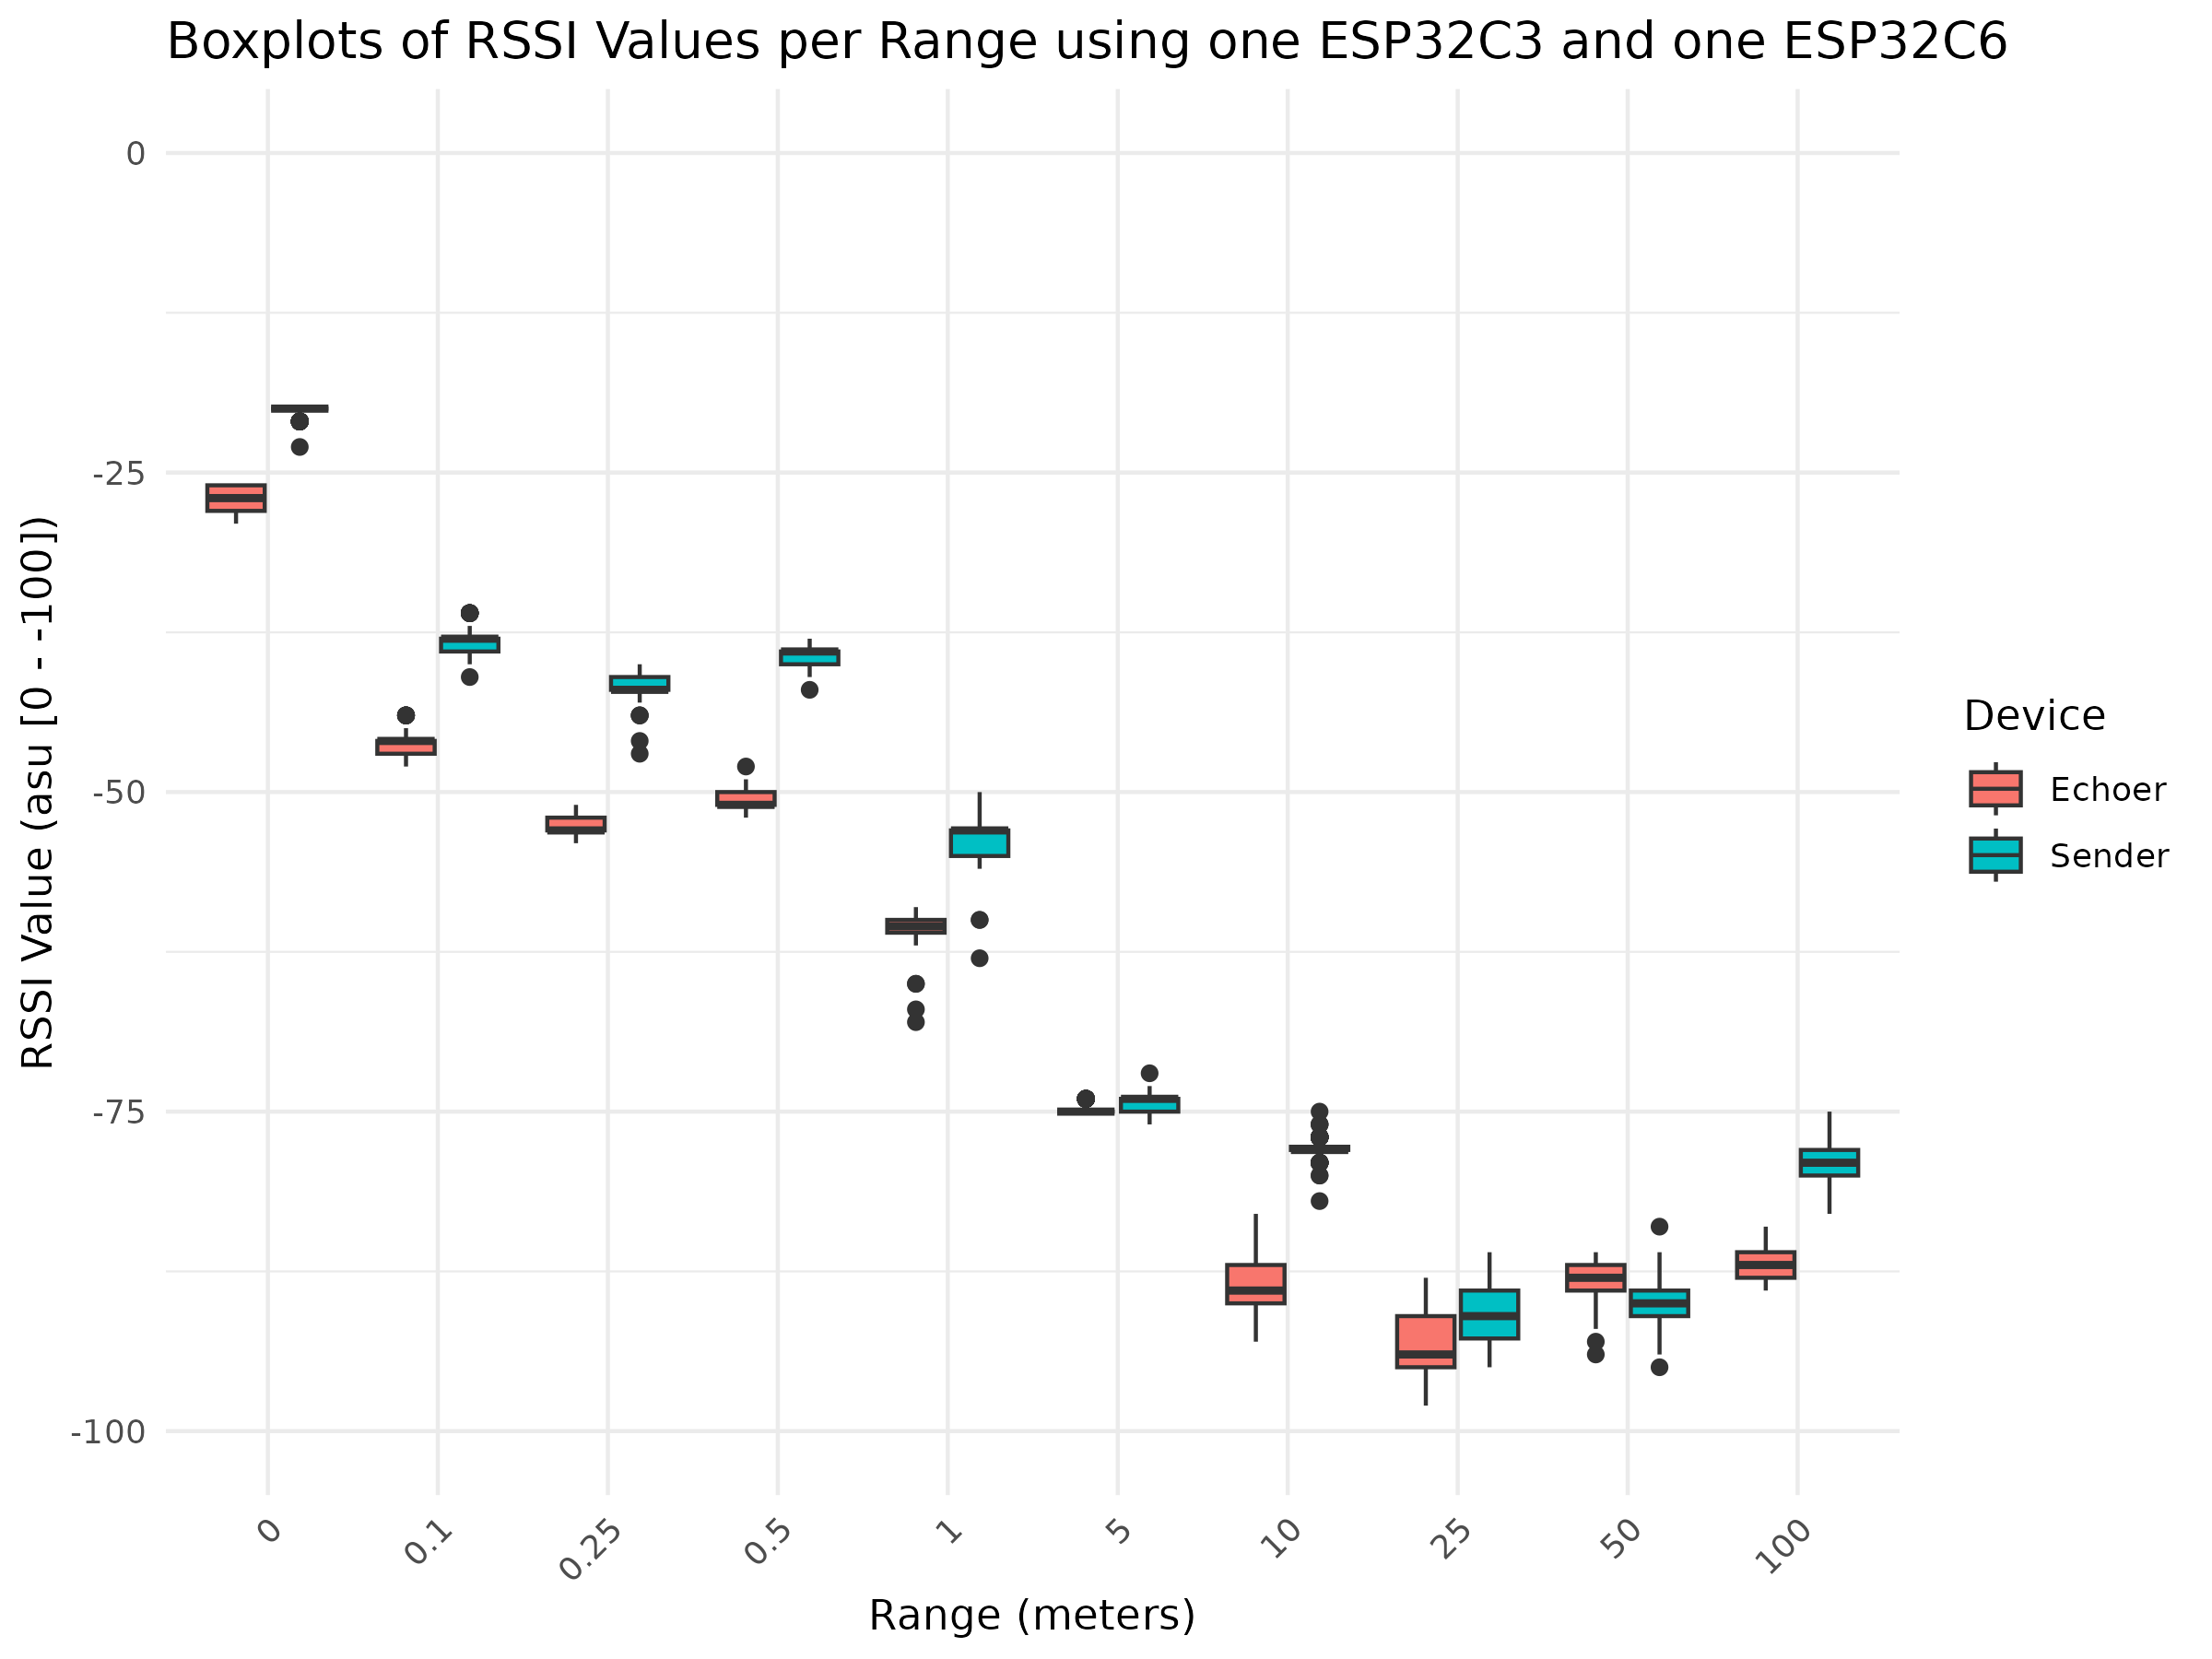
\includegraphics[width=\linewidth]{rstudio/analysis/plots/ESP32C36_rssi_box.png}
    \end{subfigure}
    \begin{subfigure}{0.45\textwidth}
        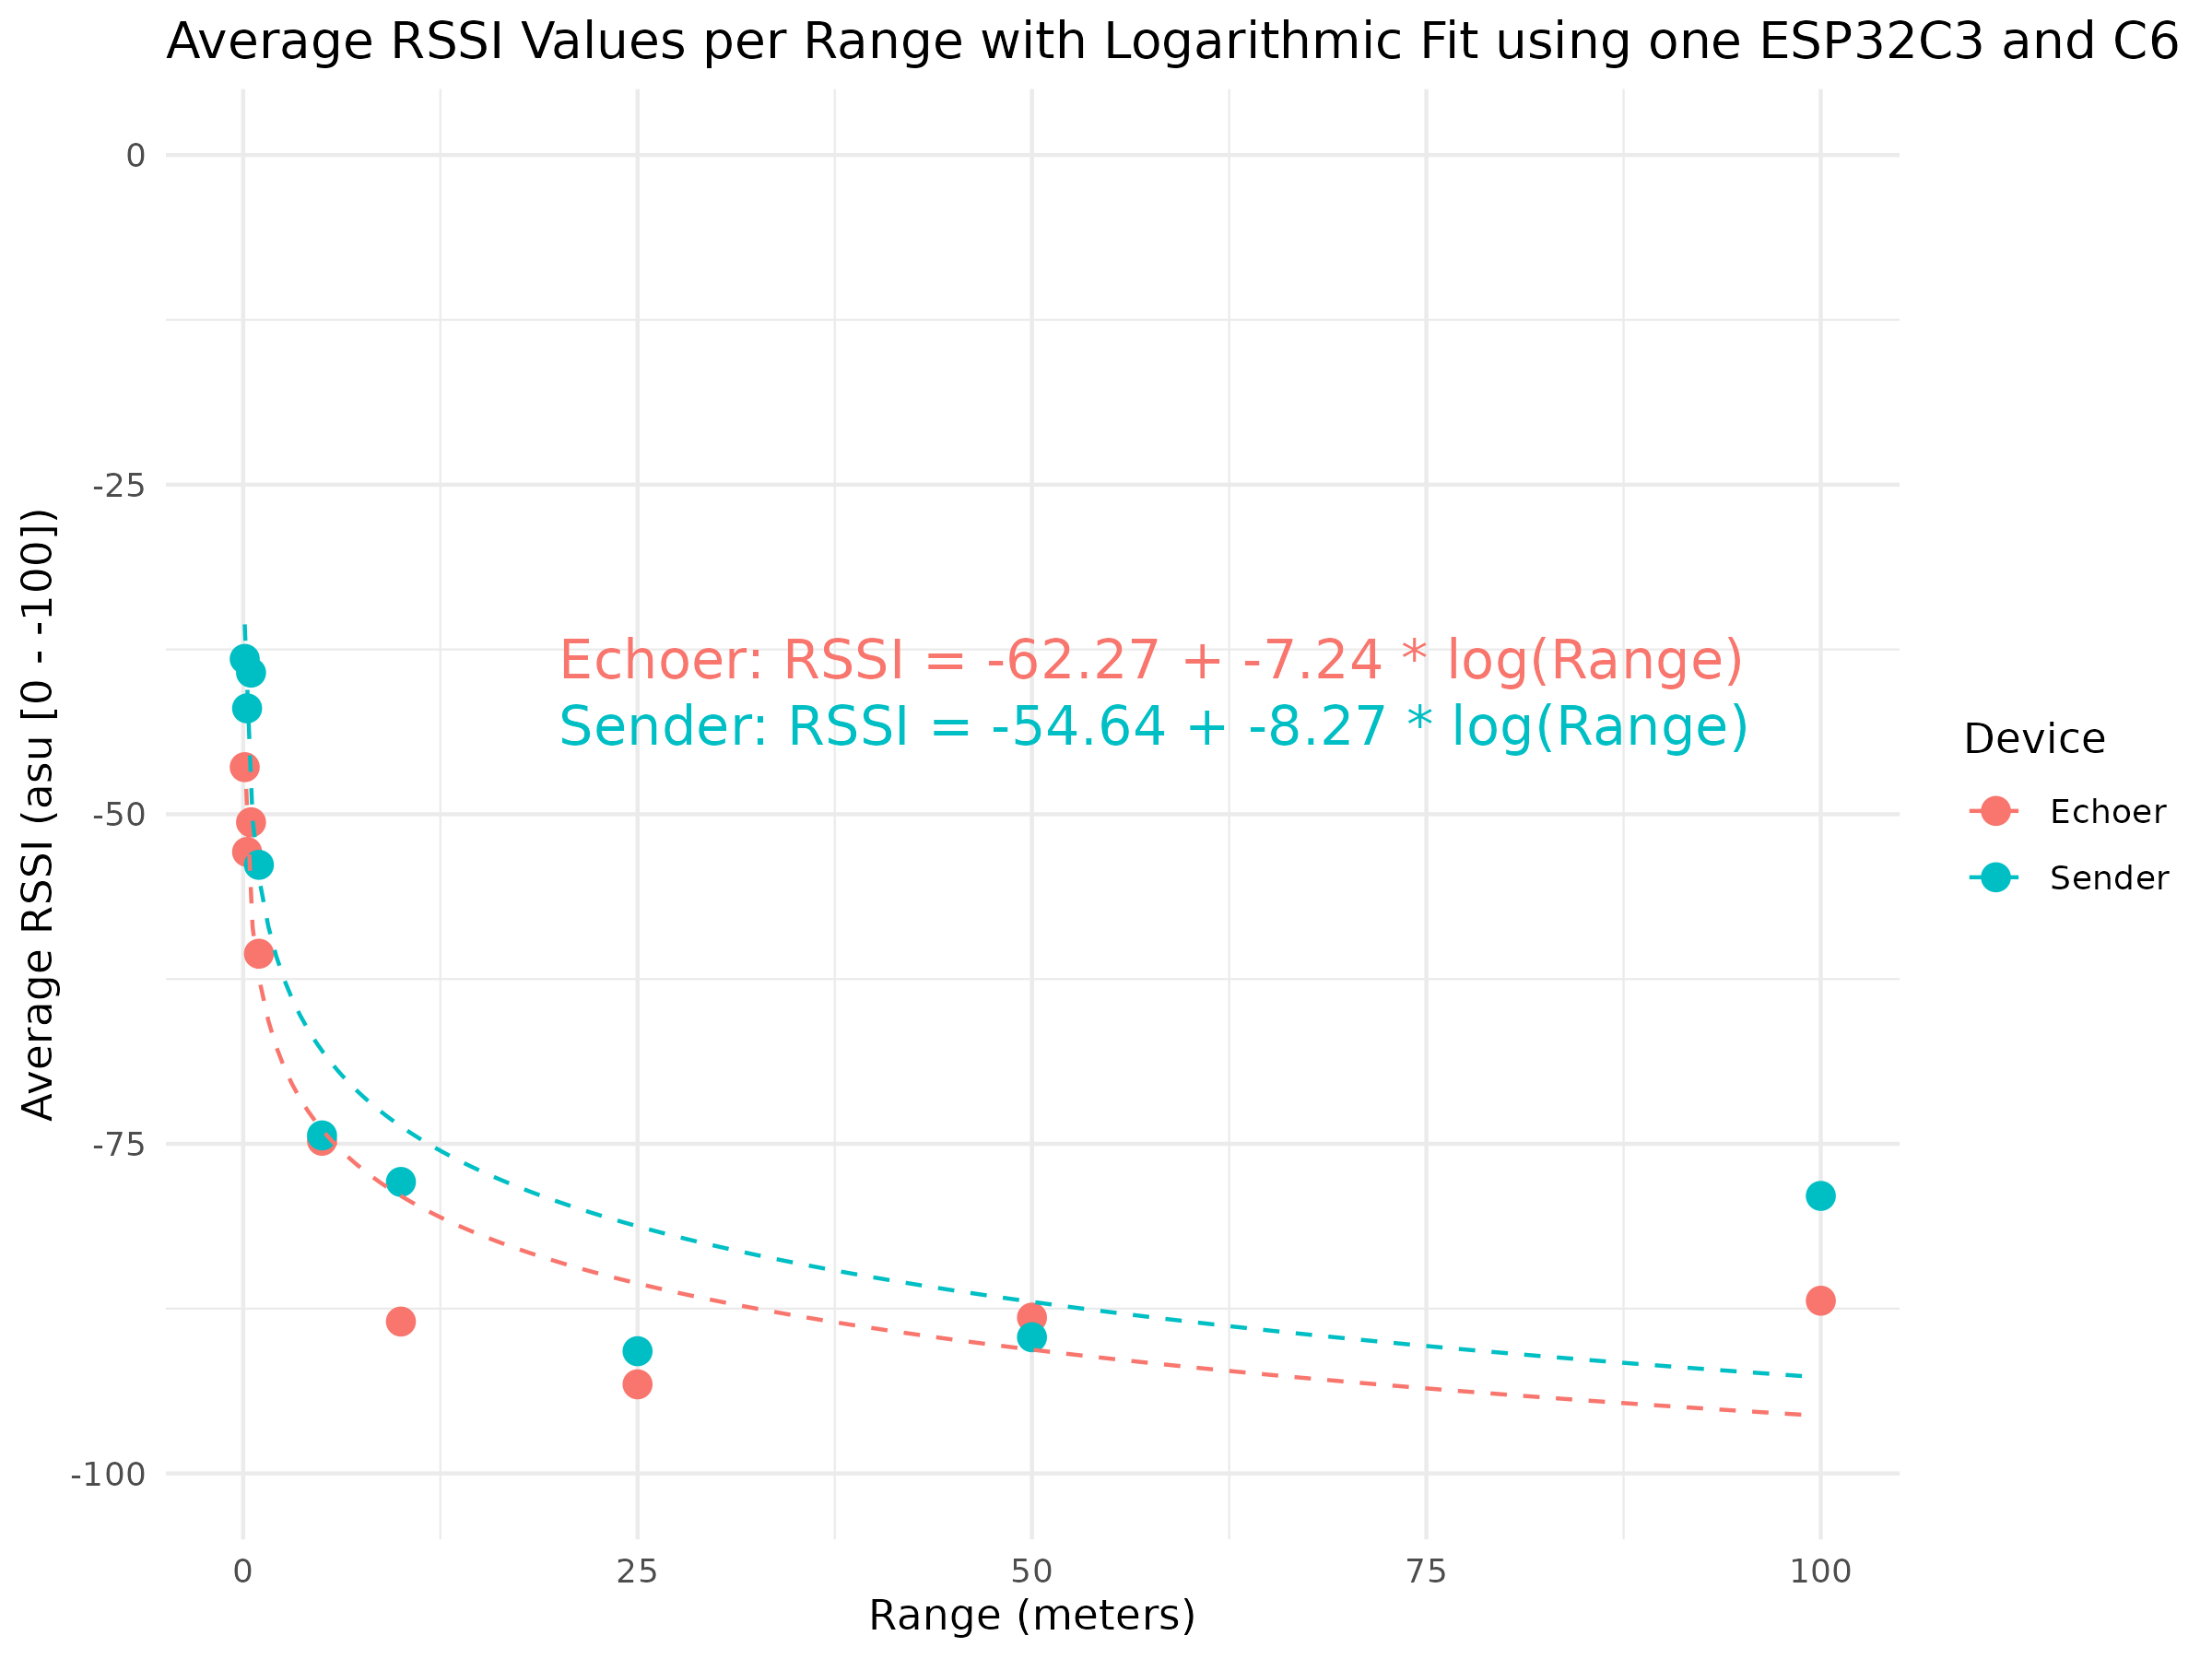
\includegraphics[width=\linewidth]{rstudio/analysis/plots/ESP32C36_avg_rssi.png}
    \end{subfigure}

    \begin{subfigure}{0.45\textwidth}
        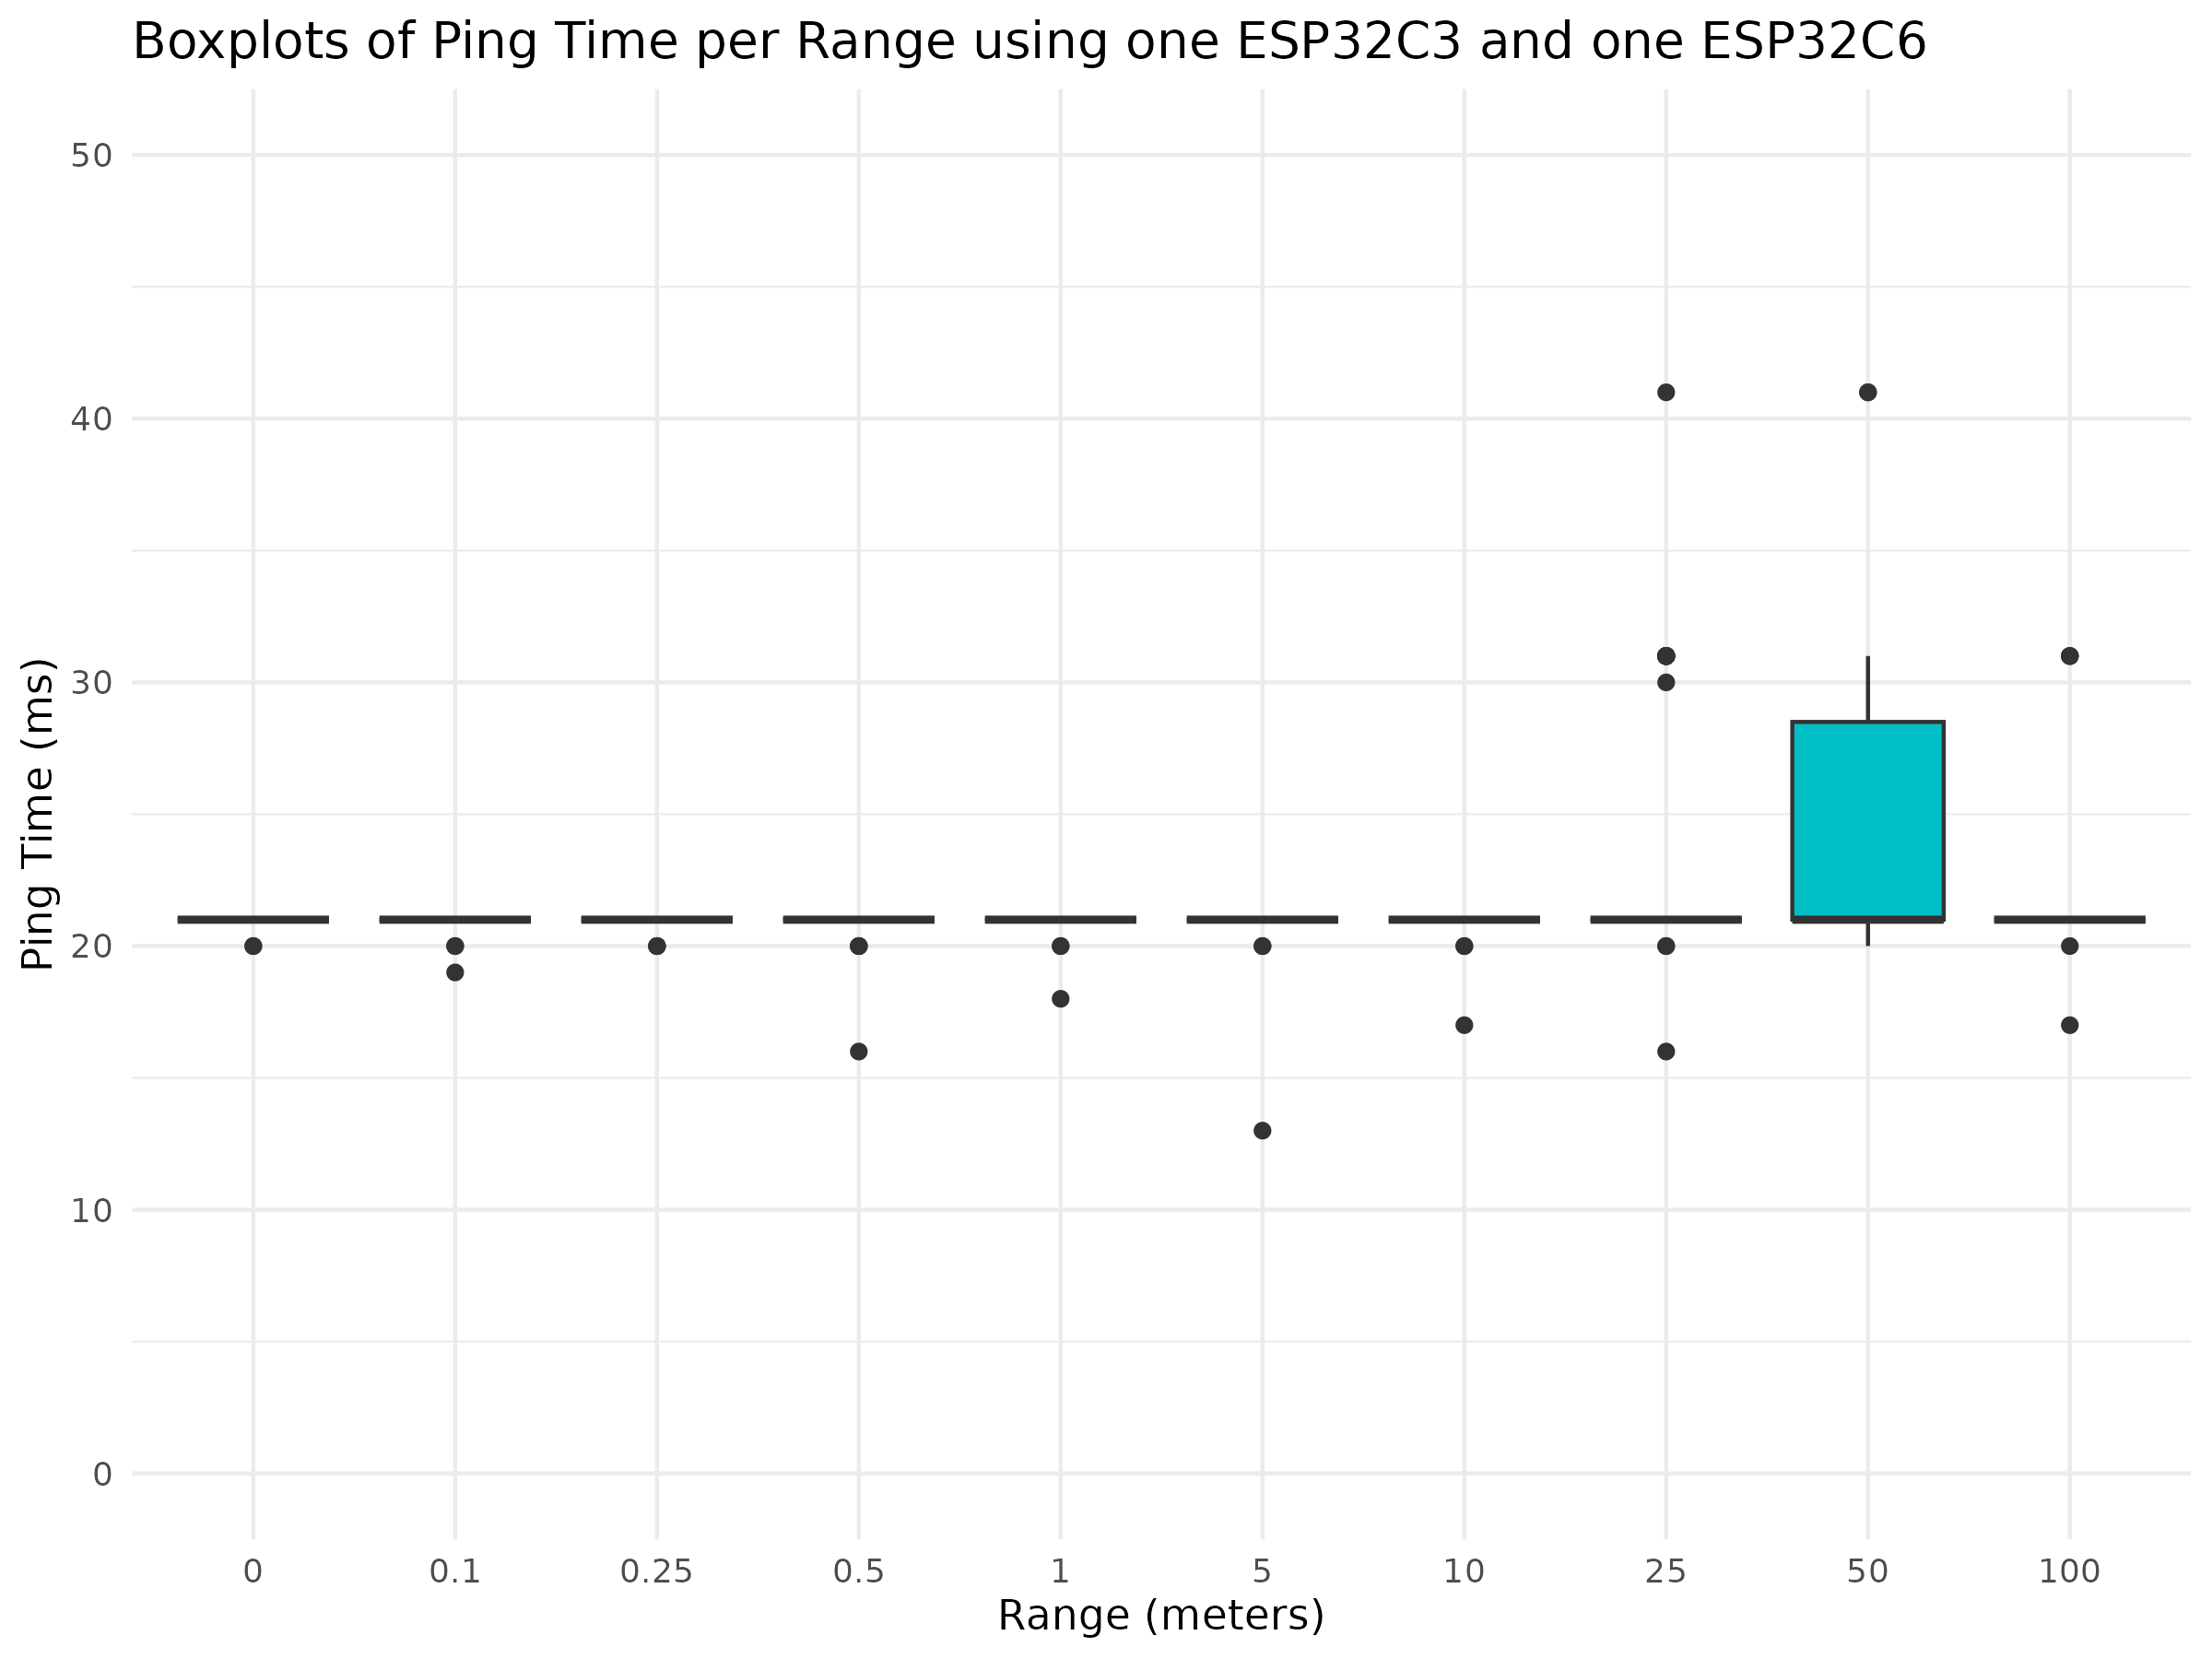
\includegraphics[width=\linewidth]{rstudio/analysis/plots/ESP32C36_ping_box.png}
    \end{subfigure}
    \begin{subfigure}{0.45\textwidth}
        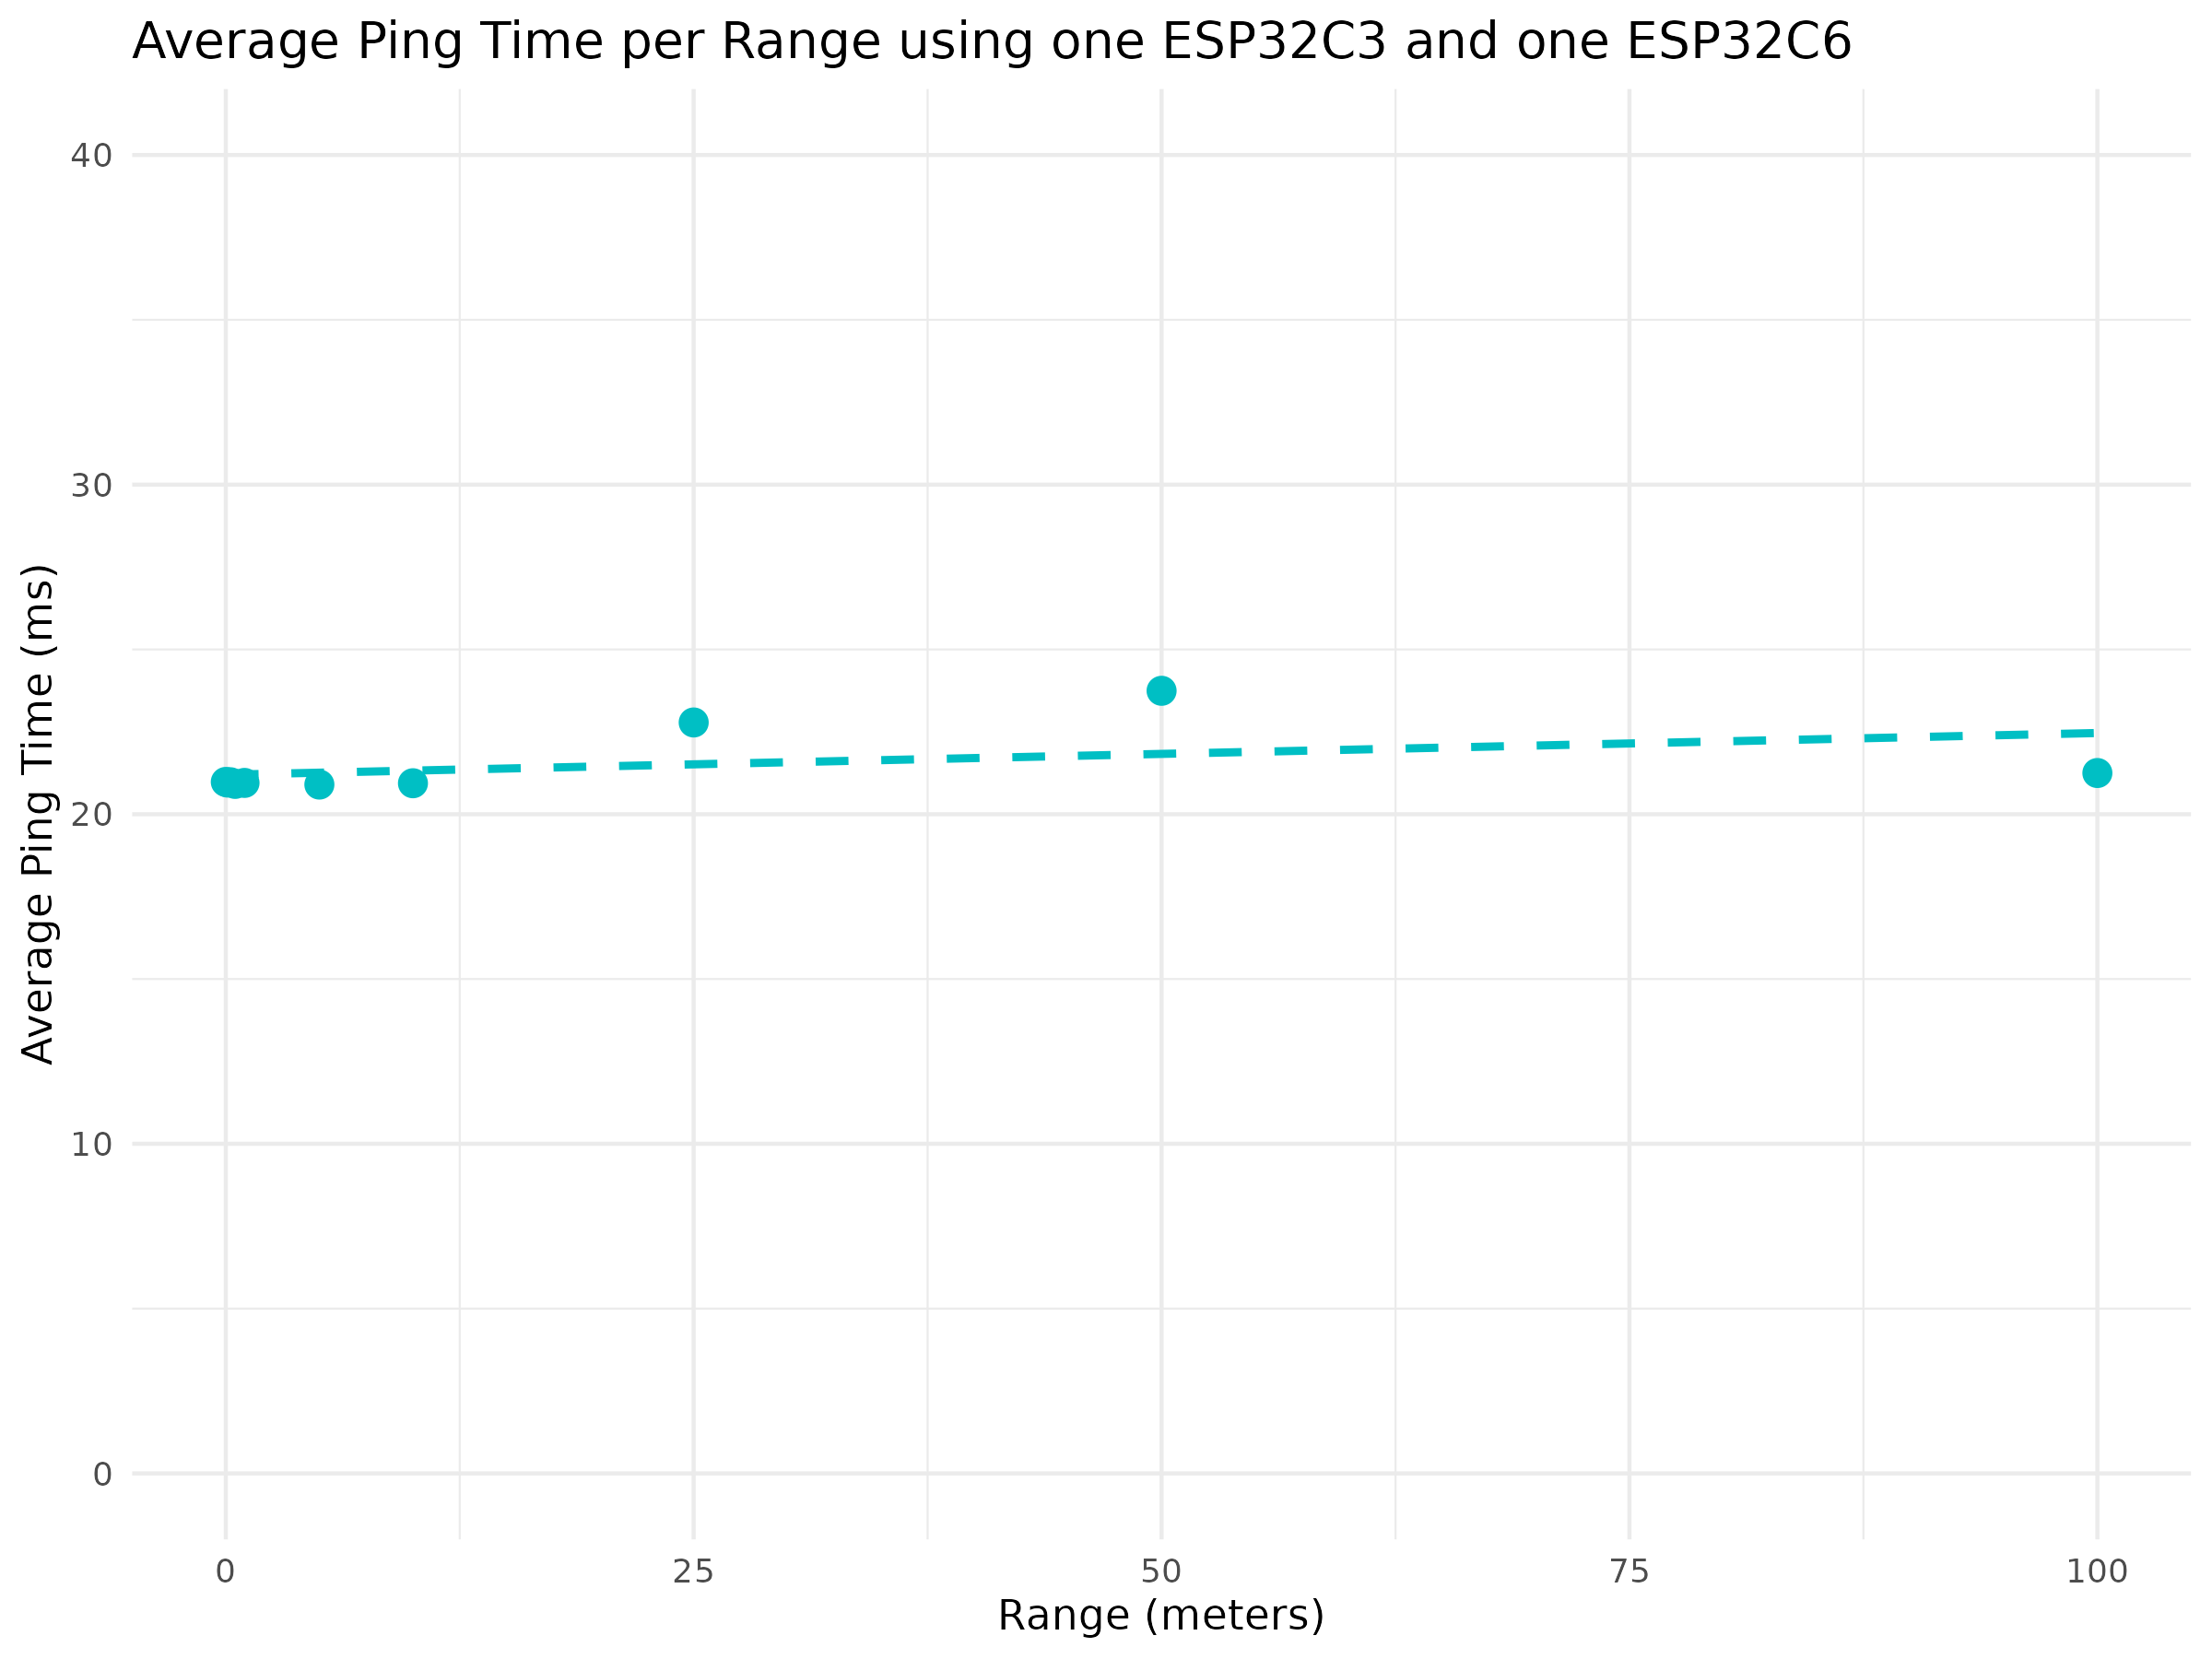
\includegraphics[width=\linewidth]{rstudio/analysis/plots/ESP32C36_avg_ping.png}
    \end{subfigure}
    \vspace{\ftspace}
    \caption{RSSI and ping response time depending on range using one ESP32C3 and one ESP32C6}
    \label{fig:rssipingrange_esp32c36}
\end{figure}

Analogous results were obtained using an ESP32C3 as the sender and an ESP32C6 as the echoer. The RSSI values followed a similar logarithmic trajectory, although in this instance the values were considerably lower for both devices, likely attributed to the smaller on-board antenna used by the ESP32C6. The RSSI values for the sender (ESP32C3) remained significantly higher for most measurements, except for the 5 meter and 50 meter measurements, where the values were found to be similar. Surprisingly, the RSSI values for 100 meters were better than both 50 and 25 meters, with the lowest values for the test occurring at 25 meters. This might be explained by the intermittent fluctuation of RSSI values. While during standard deviation remains small, repeating the same measurement at the same range one a different day, can result in different RSSI values. The underlying cause of this variability remains unclear.\\

The ping values also exhibited a uniform distribution, with an average of around $20\ ms$, with some minor outliers observed for greater distances.\\

In terms of packet loss, a parallel trend to RSSI values is observed, with packet loss at the highest for the measurement at a range of 25 meters, with a similar amount of packets lost each direction. Notably, no packets were lost for the measurement at 100 meters. \\

However, a single, isolated and unexplained inconsistency in the data is observed. Specifically for the 10 meter measurement, the echo device did not receive two packets (number 62 and 72), yet the sender did receive the return echo of these two packets. This discrepancy suggests the presence of an error, yet the raw data collected indicates that packets 62 and 72 were successfully received with a timestamp assigned to the sender. However, there are no records for these packets on the echo device. One possible explanation for this discrepancy is a bug in the test code, such as the dictionary not being cleared or reinitialised properly, retaining previous values. However, this appears improbable, as the dictionary is cleared and reinitialised empty with every new run of the code, as well as when data is written to files. Consequently, the most plausible explanation appears to be an error on the part of the echoer in writing the data to the dictionary. The echo logic and response are based on IRQ functions, so an error would not have interrupted the test and given the lack of logging, such an error may have gone unnoticed. 
\newpage

\begin{table}[H]
    \centering
    \begin{tabular}{|c|c|l|l|c|c|c|c|c|}
    \hline
        Range & Packet Loss & \multicolumn{2}{l|}{Measurement} & \multicolumn{5}{c|}{Values} \\\hline
        [meters] & [\%] & \multicolumn{2}{l|}{} & mean & std & min & max & median \\\hline\hline
        \multirow{3}{*}{0 m} & \multirow{1}{*}{0} & RSSI 1 & [asu] & -6.05 & 1.14 & -12 & -5 & -6 \\\cline{2-9}\cline{2-9}
        %&& Time 1 &  &  &  &  &  \\\cline{2-9}\cline{2-9}
        & \multirow{2}{*}{0} & RSSI 2 & [asu] & -27.13 & 0.93 & -29 & -26 & -27 \\\cline{3-9}
        %&& Time 2 &  &  &  &  &  \\\cline{3-9}
        && Ping & [ms] & 20.98 & 0.14 & 20 & 21 & 21 \\\hline\hline
        \multirow{3}{*}{0.1 m} & \multirow{1}{*}{0} & RSSI 1 & [asu] & -46.43 & 1.12 & -44 & -48 & -46 \\\cline{2-9}\cline{2-9}
        %&& Time 1 &  &  &  &  &  \\\cline{2-9}\cline{2-9}
        & \multirow{2}{*}{0} & RSSI 2 & [asu] & -38.22 & 1.04 & -41 & -36 & -38 \\\cline{3-9}
        %&& Time 2 &  &  &  &  &  \\\cline{3-9}
        && Ping & [ms] & 20.96 & 0.24 & 19 & 21 & 21 \\\hline\hline
        \multirow{3}{*}{0.25 m} & \multirow{1}{*}{0} & RSSI 1 & [asu] & -52.86 & 0.72 & -54 & -51 & -53 \\\cline{2-9}\cline{2-9}
        %&& Time 1 &  &  &  &  &  \\\\cline{2-9}\cline{2-9}
        & \multirow{2}{*}{0} & RSSI 2 & [asu] & -41.97 & 1.02 & -47 & -40 & -42 \\\cline{3-9}
        %&& Time 2 &  &  &  &  &  \\\cline{3-9}
        && Ping & [ms] & 20.97 & 0.17 & 20 & 21 & 21 \\\hline\hline
        \multirow{3}{*}{0.5 m} & \multirow{1}{*}{0} & RSSI 1 & [asu] & -50.61 & 0.72 & -52 & -48 & -51 \\\cline{2-9}\cline{2-9}
        %&& Time 1 &  &  &  &  &  \\\cline{2-9}\cline{2-9}
        & \multirow{2}{*}{0} & RSSI 2 & [asu] & -39.26 & 0.66 & -42 & -38 & -39 \\\cline{3-9}
        %&& Time 2 &  &  &  &  &  \\\cline{3-9}
        && Ping & [ms] & 20.92 & 0.52 & 16 & 21 & 21 \\\hline\hline
        \multirow{3}{*}{1 m} & \multirow{1}{*}{0} & RSSI 1 & [asu] & -60.58 & 1.39 & -68 & -59 & -60.5 \\\cline{2-9}\cline{2-9}
        %&& Time 1 &  &  &  &  &  \\\cline{2-9}\cline{2-9}
        & \multirow{2}{*}{0} & RSSI 2 & [asu] & -53.84 & 1.6 & -63 & -50 & -53 \\\cline{3-9}
        %&& Time 2 &  &  &  &  &  \\\cline{3-9}
        && Ping & [ms] & 20.95 & 0.33 & 18 & 21 & 21 \\\hline\hline
        \multirow{3}{*}{5 m} & \multirow{1}{*}{0} & RSSI 1 & [asu] & -74.77 & 0.42 & -75 & -74 & -75 \\\cline{2-9}\cline{2-9}
        %&& Time 1 &  &  &  &  &  \\\cline{2-9}\cline{2-9}
        & \multirow{2}{*}{0} & RSSI 2 & [asu] & -74.36 & 0.76 & -76 & -72 & -74 \\\cline{3-9}
        %&& Time 2 &  &  &  &  &  \\\cline{3-9}
        && Ping & [ms] & 20.9 & 0.81 & 13 & 21 & 21 \\\hline\hline
        \multirow{3}{*}{10 m} & \multirow{1}{*}{2} & RSSI 1 & [asu] & -88.48 & 2.02 & -93 & -83 & -89 \\\cline{2-9}\cline{2-9}
        %&& Time 1 &  &  &  &  &  \\\cline{2-9}\cline{2-9}
        & \multirow{2}{*}{0} & RSSI 2 & [asu] & -77.89 & 0.87 & -82 & -75 & -78 \\\cline{3-9}
        %&& Time 2 &  &  &  &  &  \\\cline{3-9}
        && Ping & [ms] & 20.94 & 0.42 & 17 & 21 & 21 \\\hline\hline
        \multirow{3}{*}{25 m} & \multirow{1}{*}{17} & RSSI 1 & [asu] & -93.24 & 2.51 & -98 & -88 & -94 \\\cline{2-9}\cline{2-9}
        %&& Time 1 &  &  &  &  &  \\\cline{2-9}\cline{2-9}
        & \multirow{2}{*}{26} & RSSI 2 & [asu] & -90.73 & 1.33 & -95 & -86 & -91 \\\cline{3-9}
        %&& Time 2 &  &  &  &  &  \\\cline{3-9}
        && Ping & [ms] & 22.78 & 4.31 & 16 & 41 & 21 \\\hline\hline
        \multirow{3}{*}{50 m} & \multirow{1}{*}{0} & RSSI 1 & [asu] & -88.18 & 1.49 & -94 & -86 & -88 \\\cline{2-9}\cline{2-9}
        %&& Time 1 &  &  &  &  &  \\\\cline{2-9}\cline{2-9}
        & \multirow{2}{*}{6} & RSSI 2 & [asu] & -89.67 & 1.73 & -95 & -84 & -90 \\\cline{3-9}
        %&& Time 2 &  &  &  &  &  \\\cline{3-9}
        && Ping & [ms] & 23.74 & 4.94 & 20 & 41 & 21 \\\hline\hline
        \multirow{3}{*}{100 m} & \multirow{1}{*}{0} & RSSI 1 & [asu] & -86.9 & 1.17 & -89 & -84 & -87 \\\cline{2-9}\cline{2-9}
        %&& Time 1 &  &  &  &  &  \\\cline{2-9}\cline{2-9}
        & \multirow{2}{*}{0} & RSSI 2 & [asu] & -78.95 & 1.6 & -83 & -75 & -79 \\\cline{3-9}
        %&& Time 2 &  &  &  &  &  \\\cline{3-9}
        && Ping & [ms] & 21.25 & 1.76 & 17 & 31 & 21 \\\hline
    \end{tabular}
    \vspace{\ftspace}
    \caption{RSSI, ping response time and packet loss measurements for various ranges using one ESP32C3 and one ESP32C6}
    \label{tab:rssipingrange_esp32c36}
\end{table}

\subsubsection{ESP32C6 to ESP32C6}

\begin{figure}[H]
    \centering
    \begin{subfigure}{0.45\textwidth}
        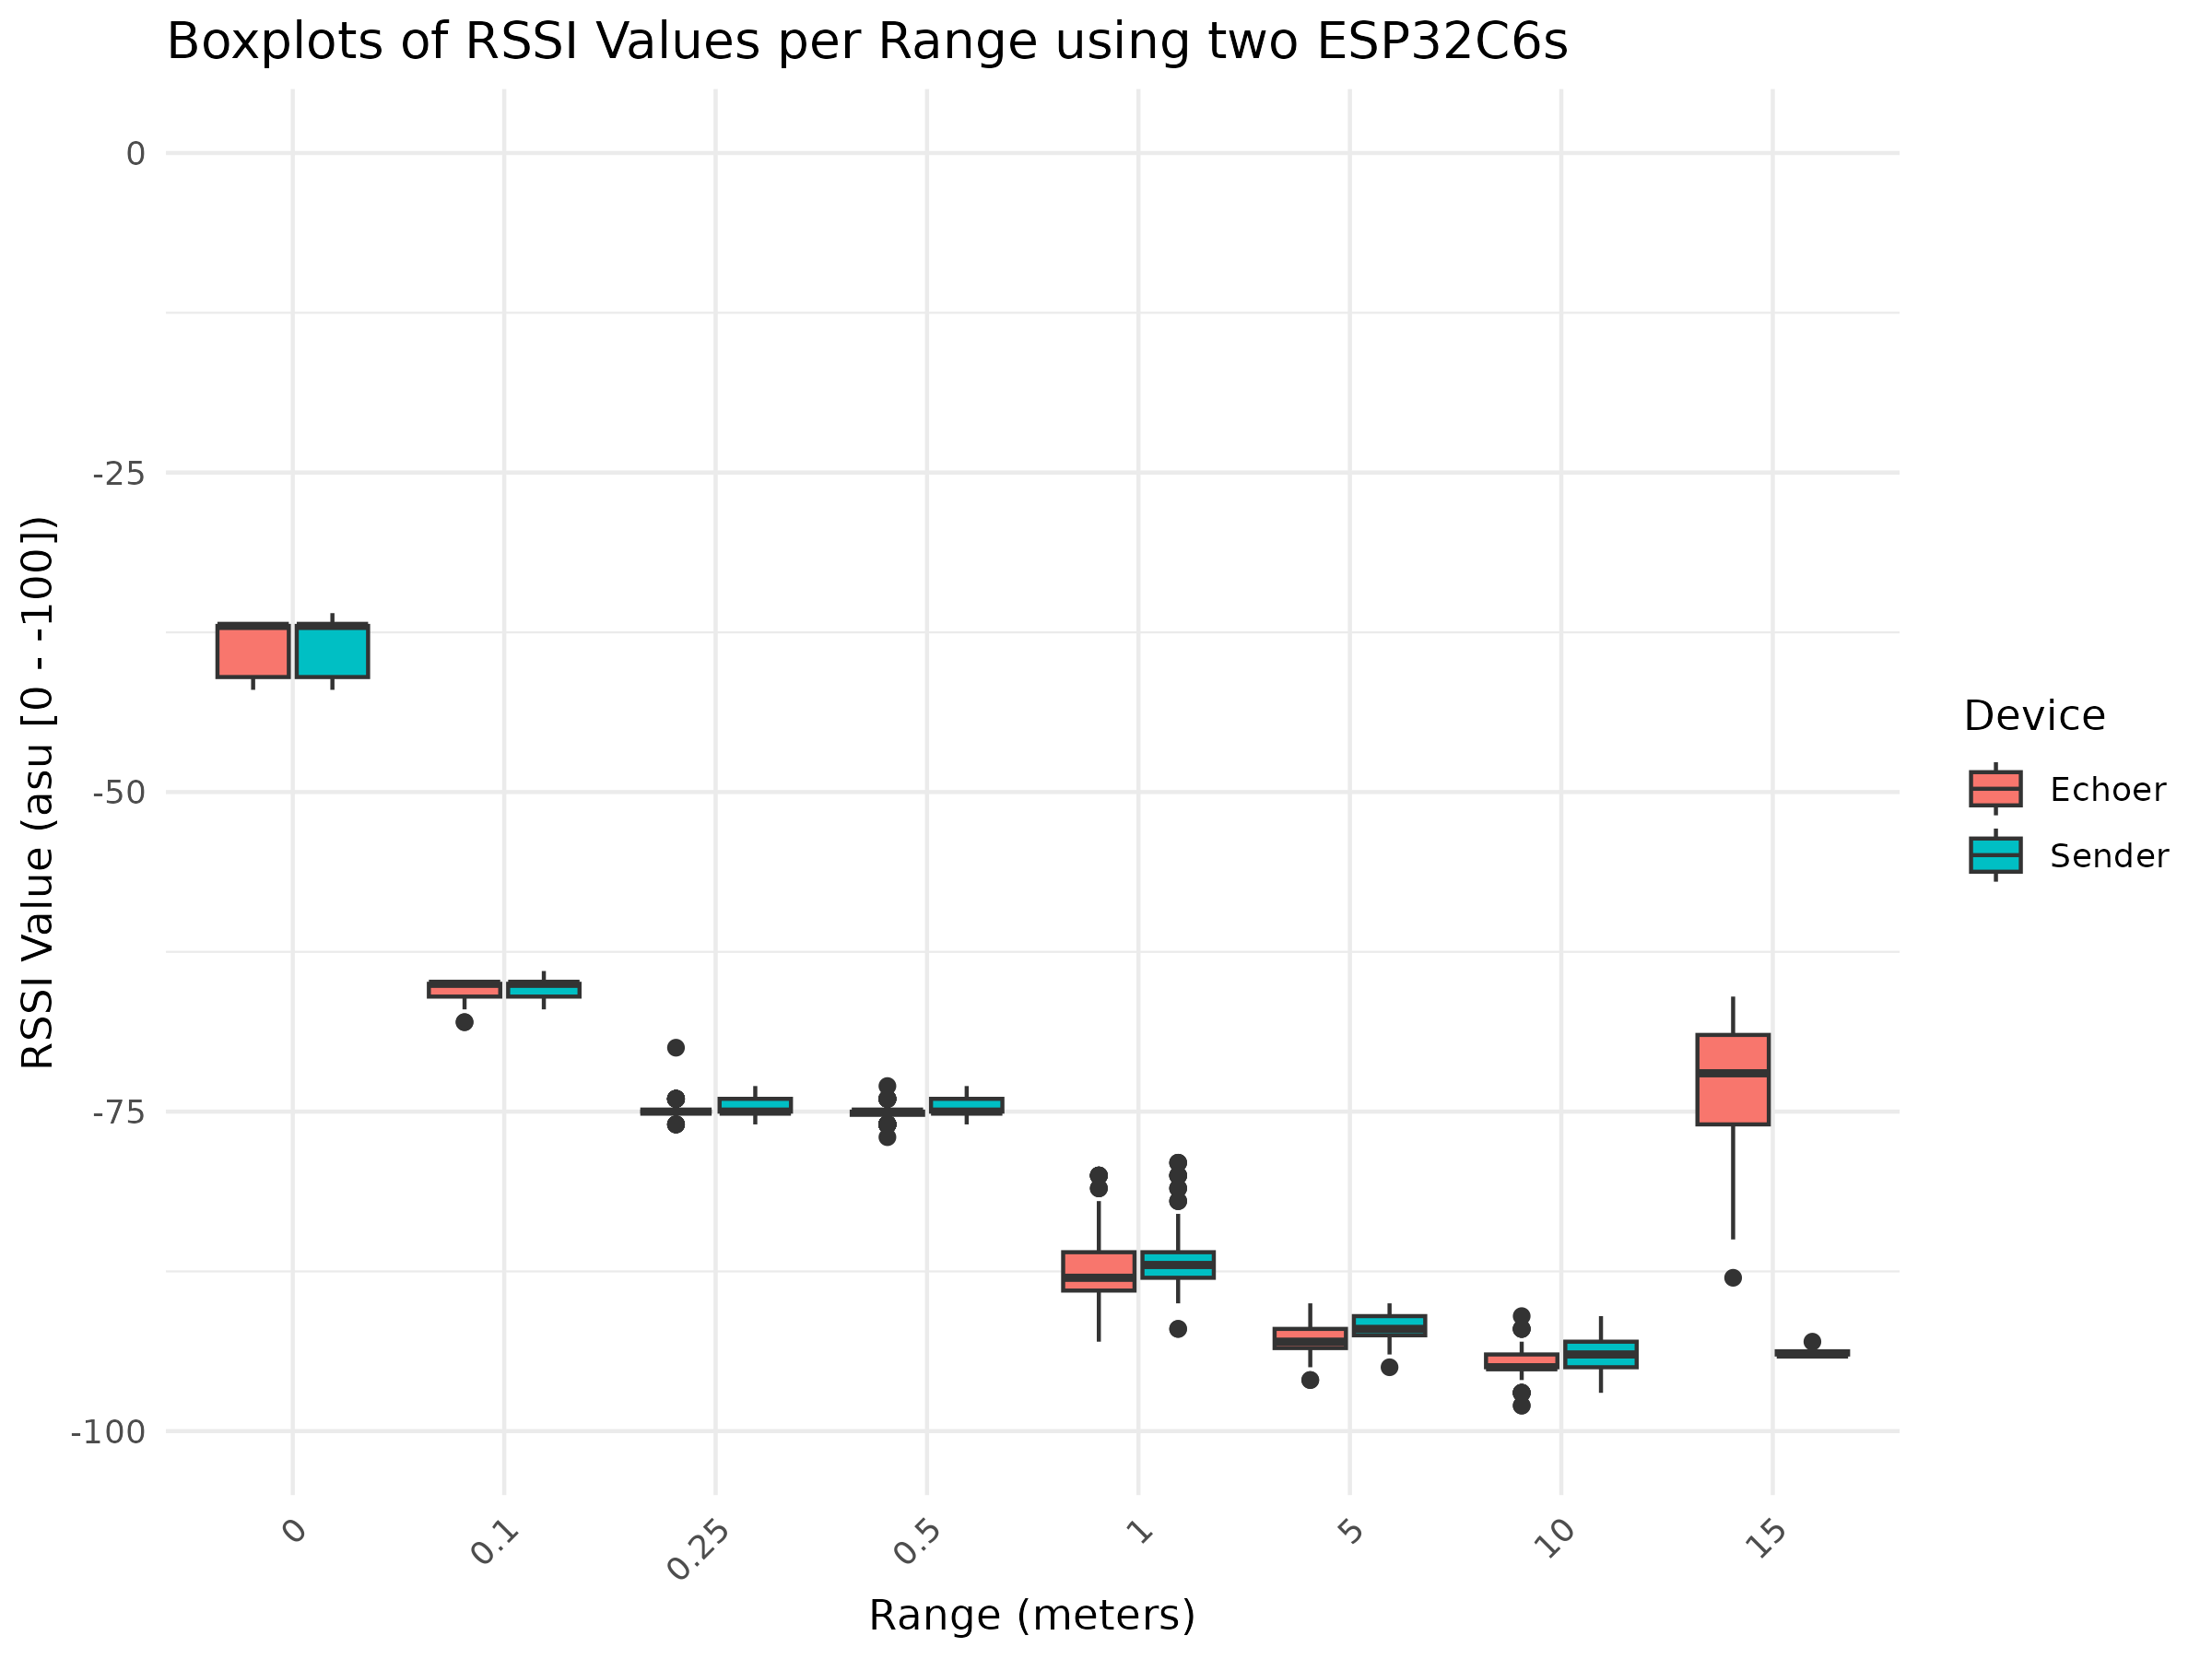
\includegraphics[width=\linewidth]{rstudio/analysis/plots/ESP32C6_rssi_box.png}
    \end{subfigure}
    \begin{subfigure}{0.45\textwidth}
        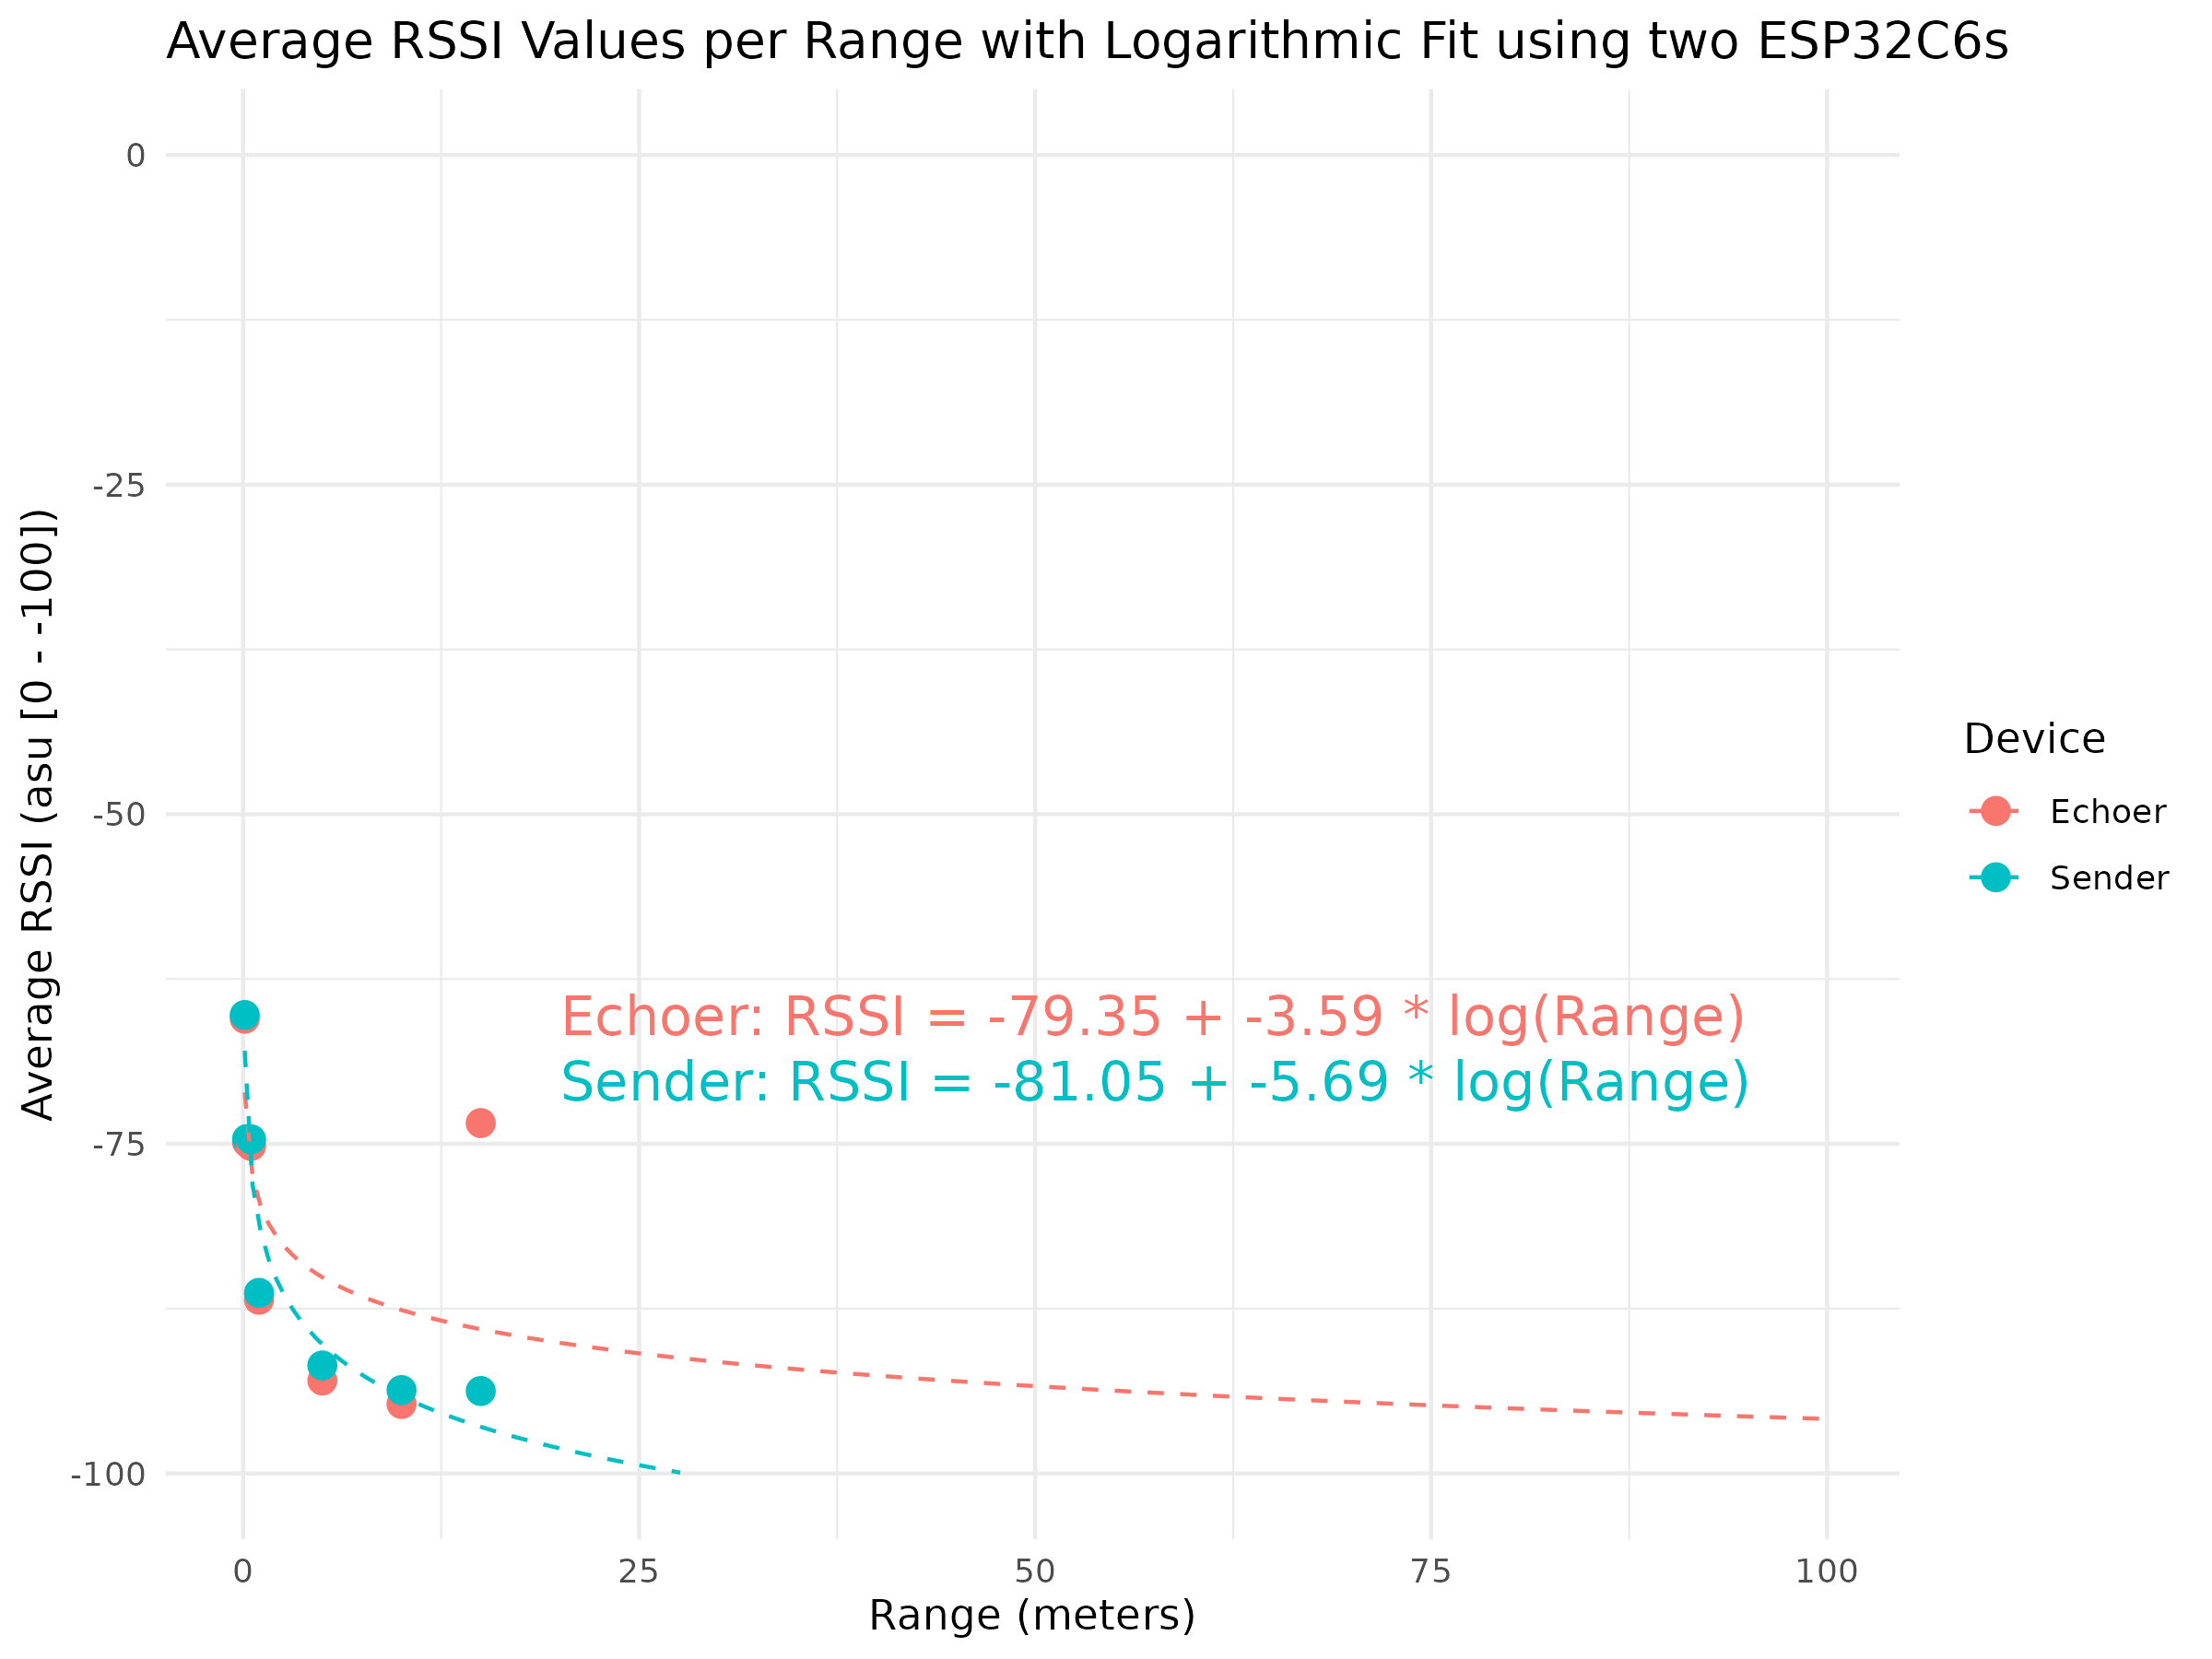
\includegraphics[width=\linewidth]{rstudio/analysis/plots/ESP32C6_avg_rssi.png}
    \end{subfigure}

    \begin{subfigure}{0.45\textwidth}
        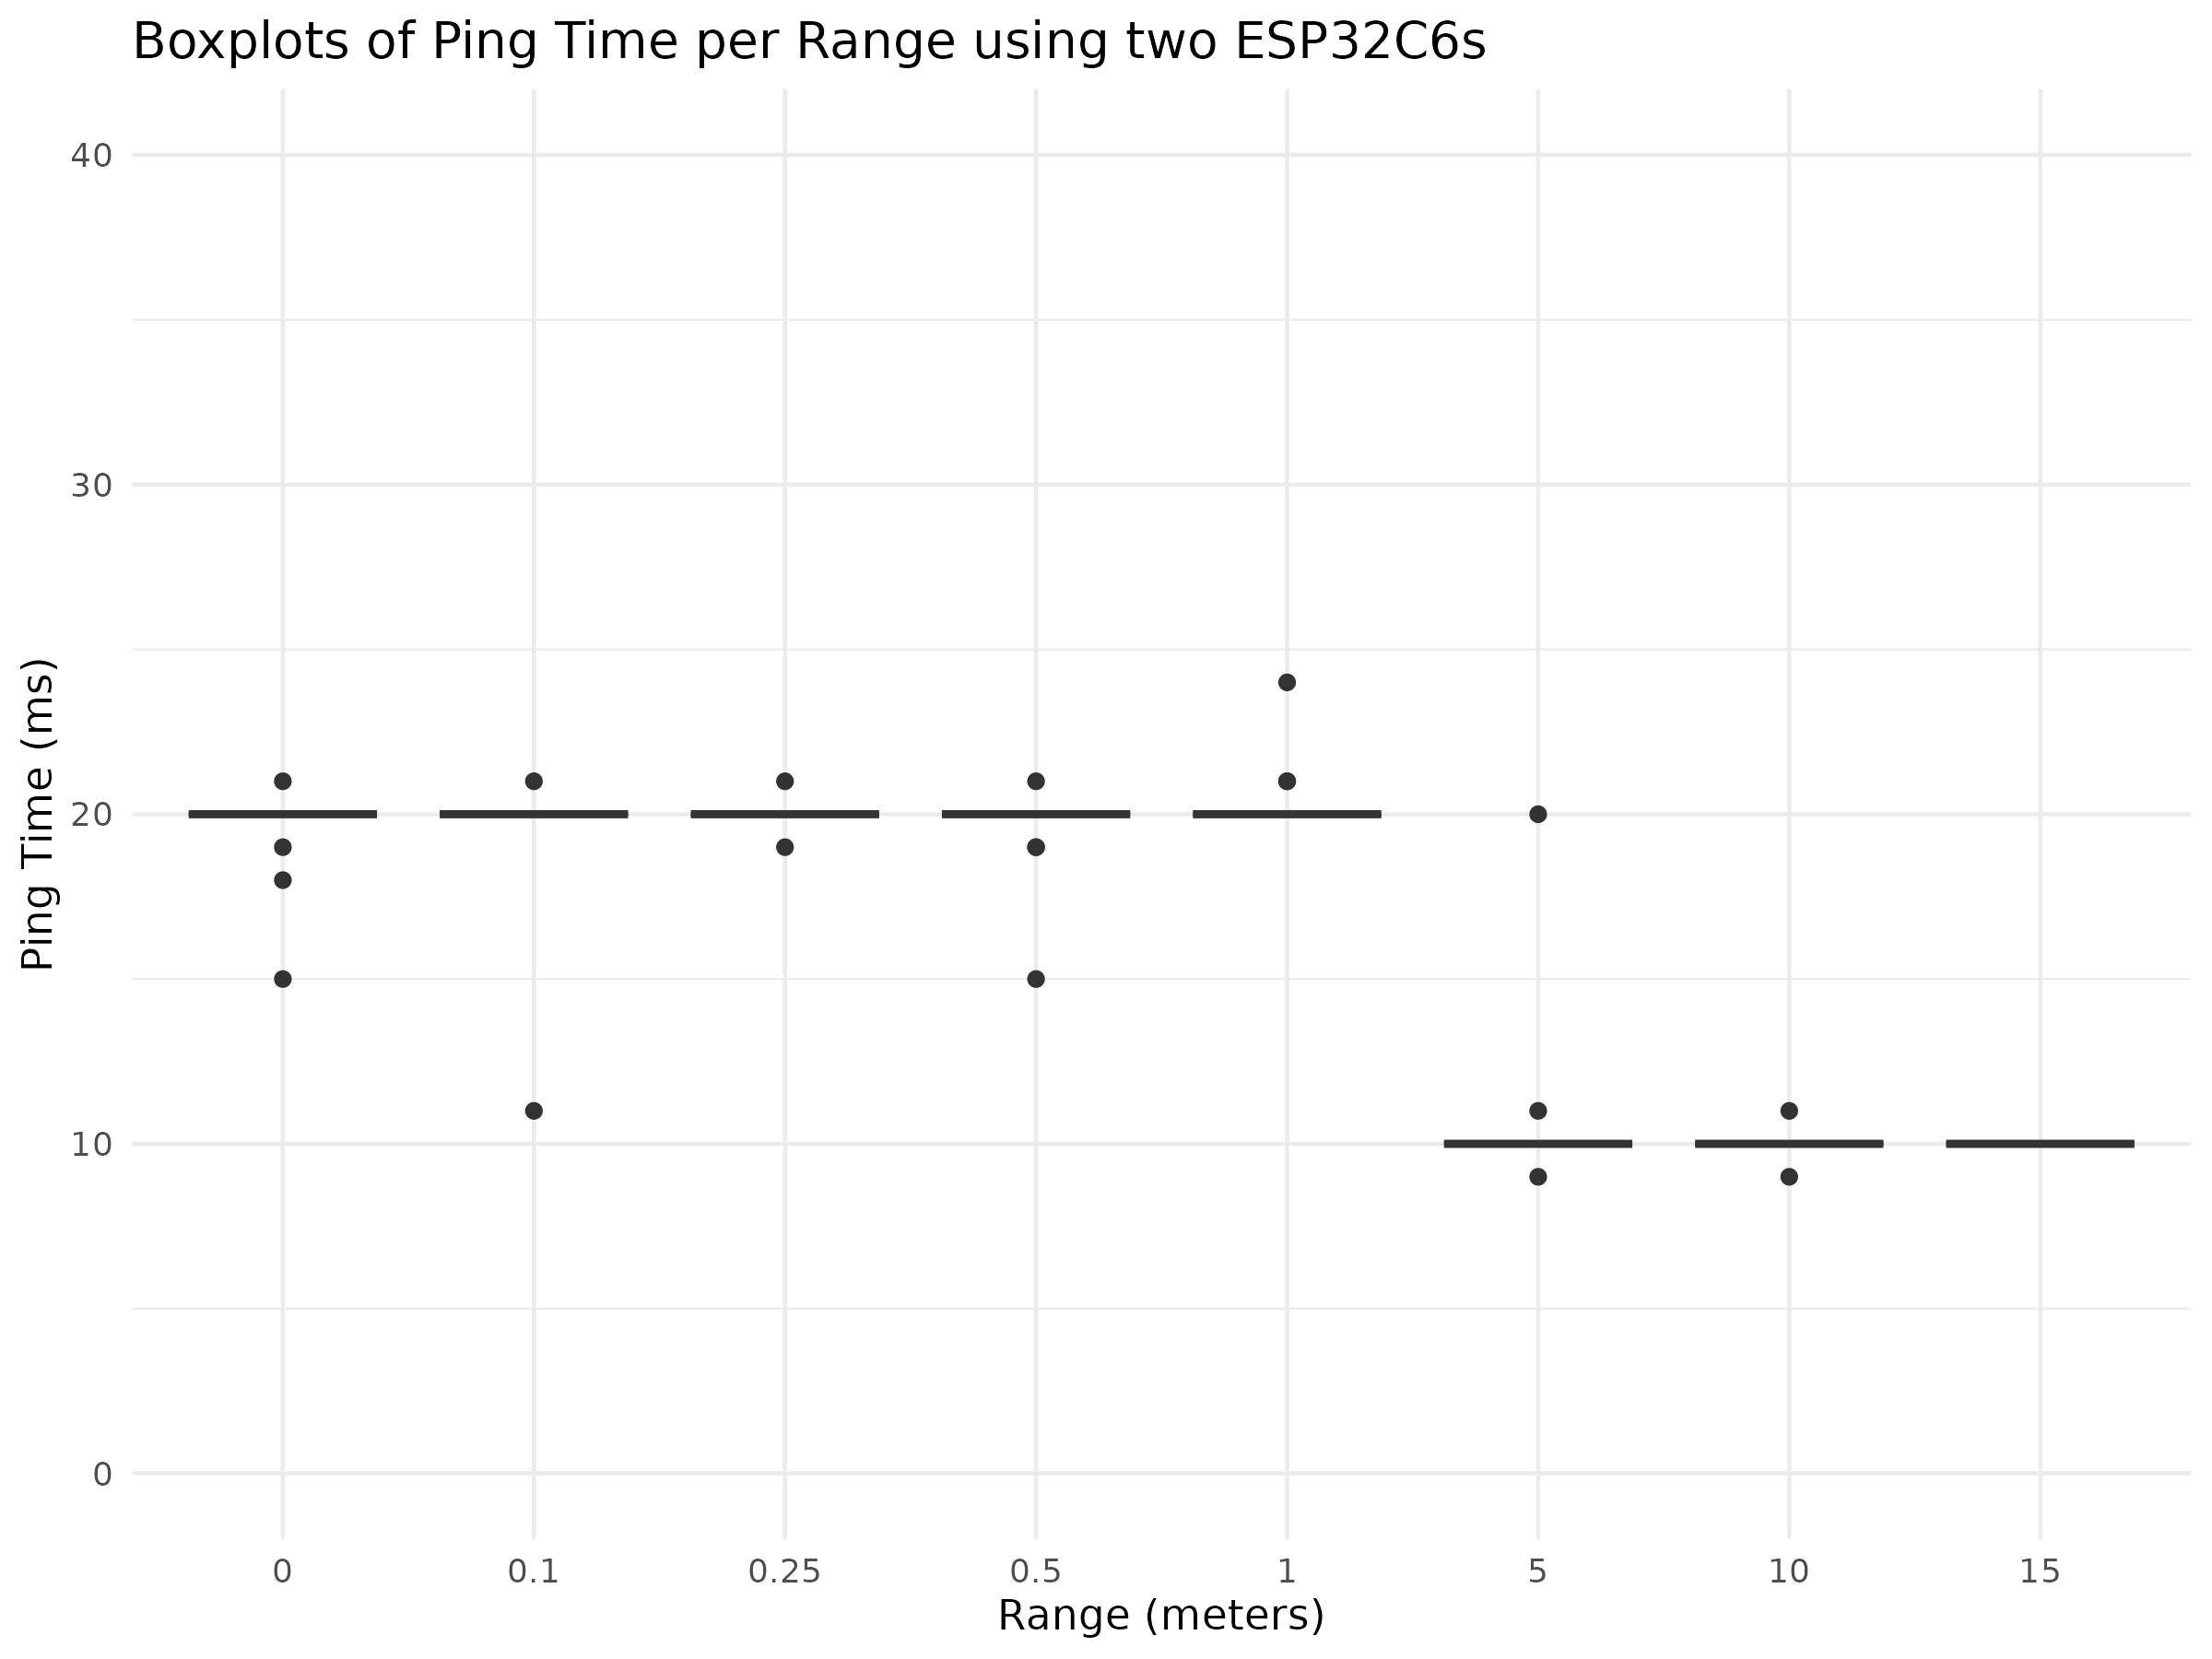
\includegraphics[width=\linewidth]{rstudio/analysis/plots/ESP32C6_ping_box.png}
    \end{subfigure}
    \begin{subfigure}{0.45\textwidth}
        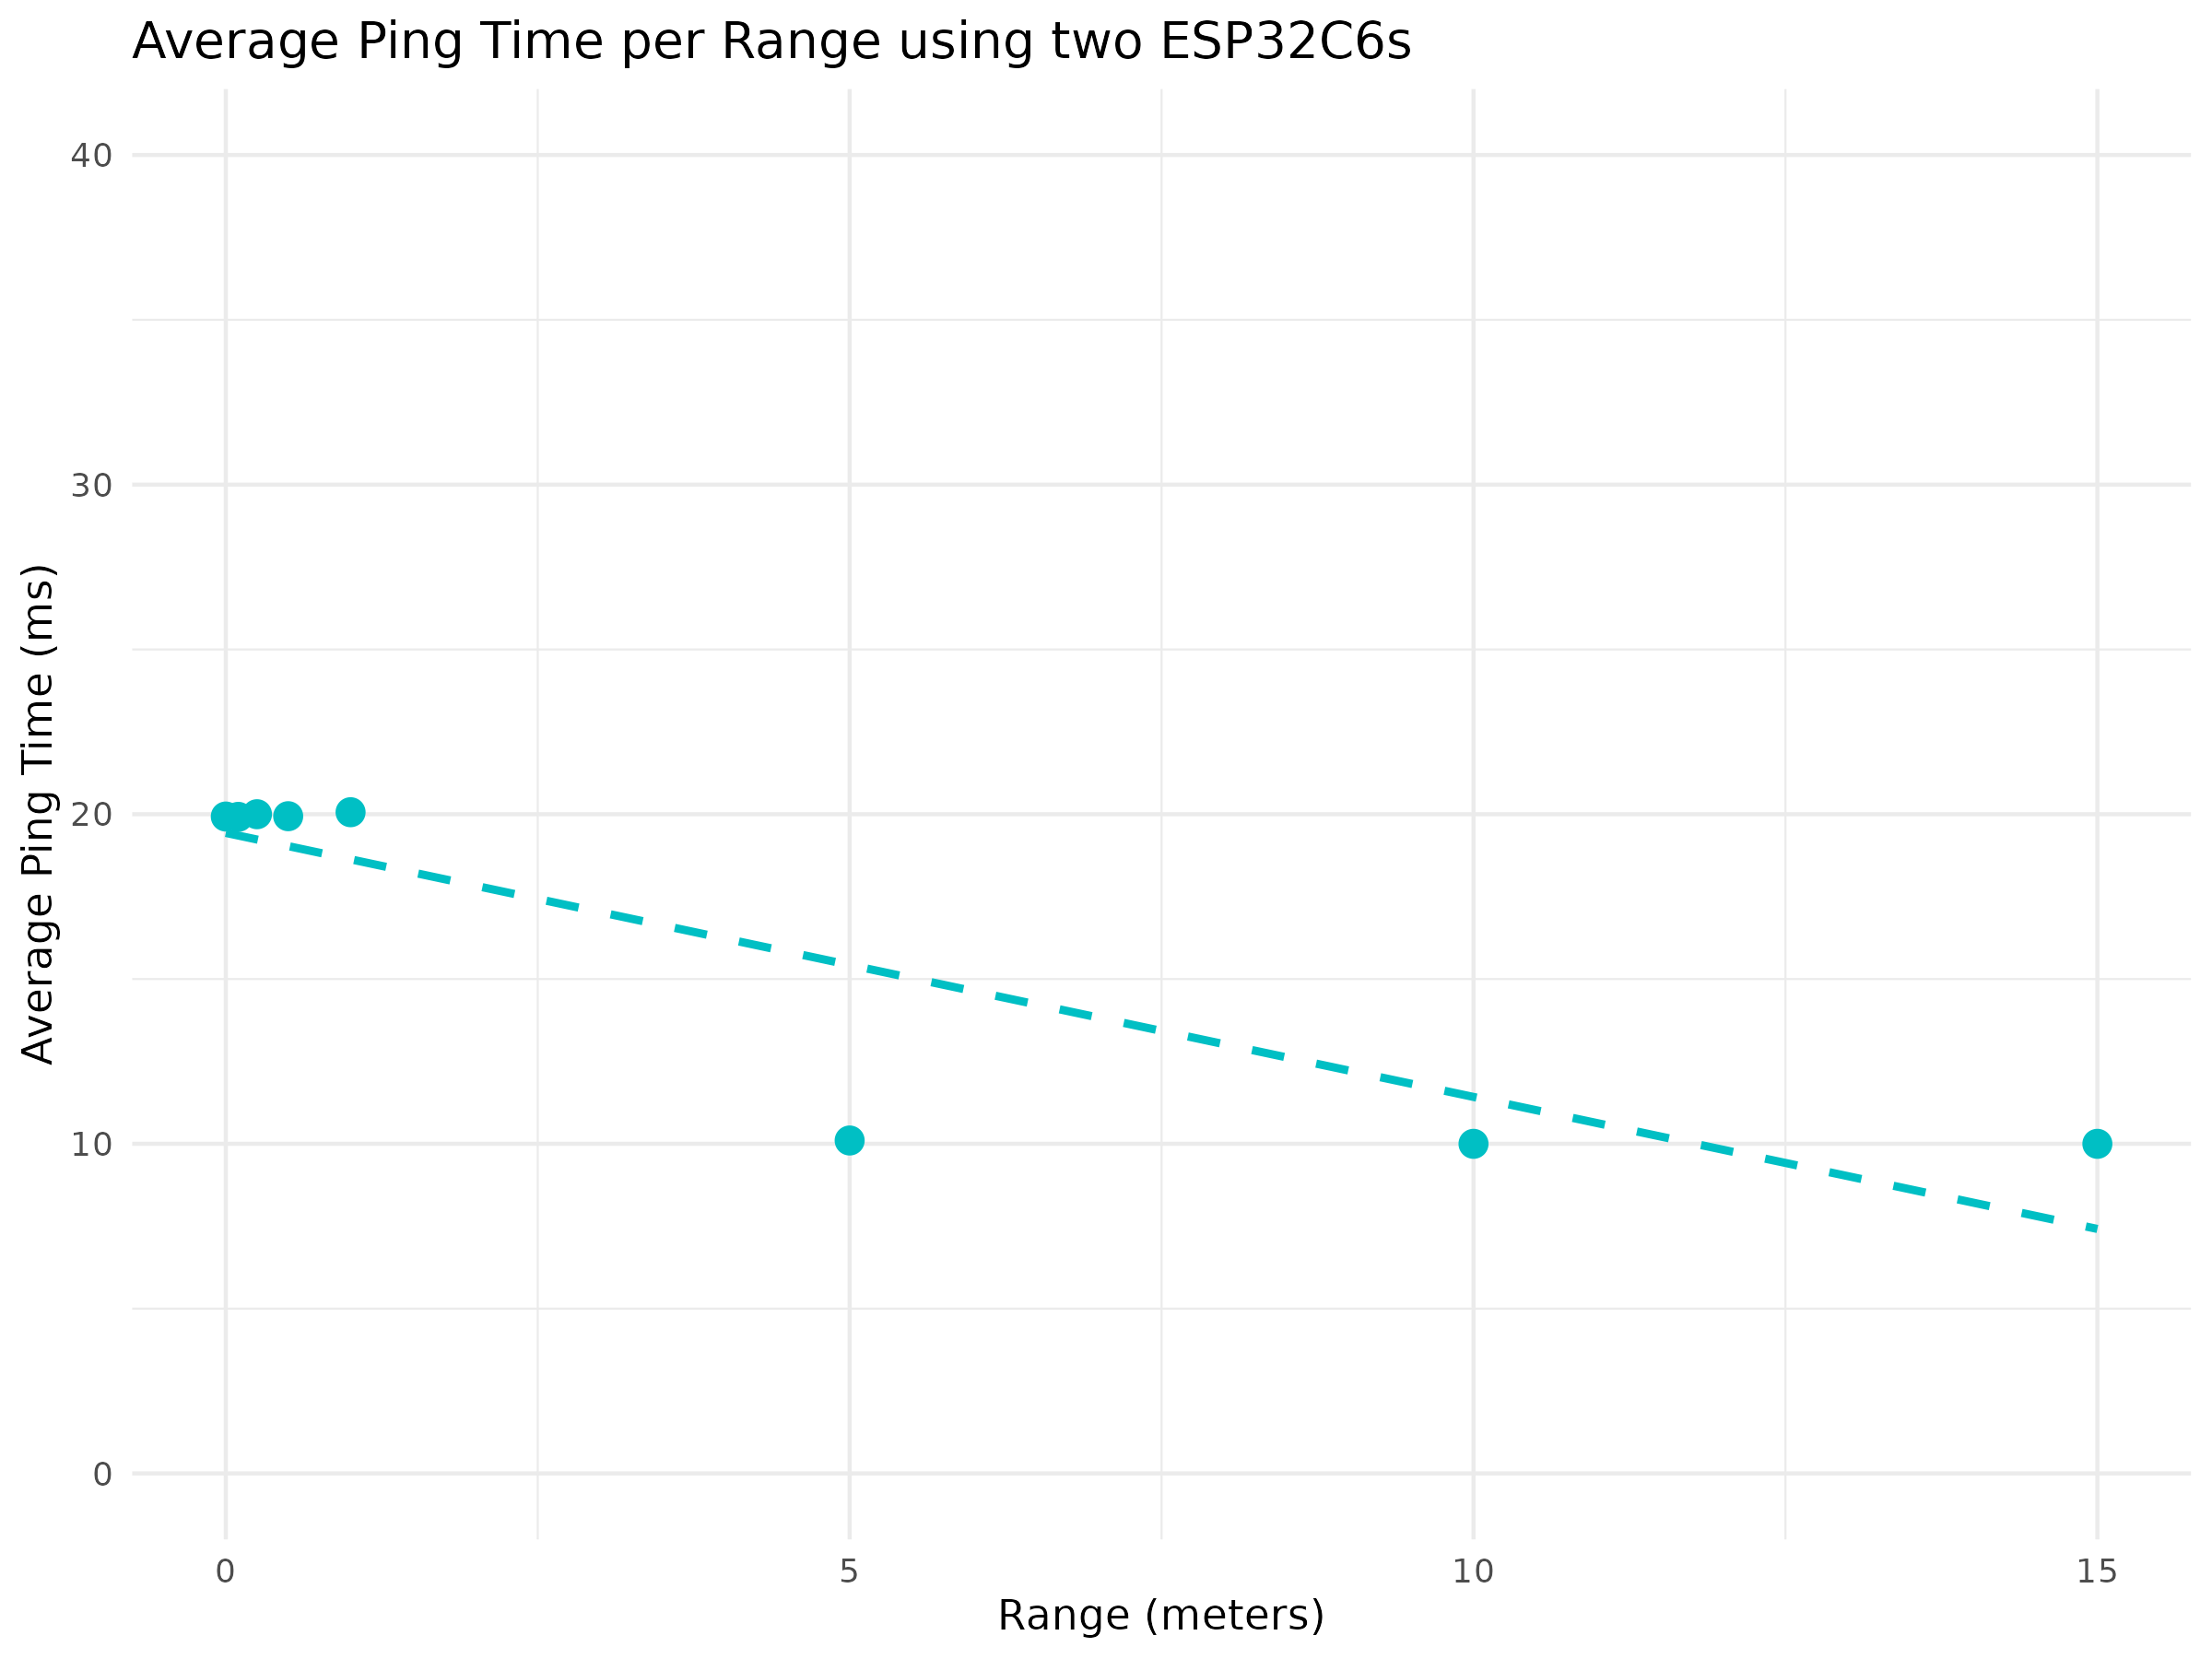
\includegraphics[width=\linewidth]{rstudio/analysis/plots/ESP32C6_avg_ping.png}
    \end{subfigure}
    \vspace{\ftspace}
    \caption{RSSI and ping response time depending on range using two ESP32C6s}
    \label{fig:rssipingrange_esp32c6}
\end{figure}

However, repeating the same test with two ESP32C6s, difficulties were encountered with transmission over a distance exceeding 15 meters. As transmission with an ESP32C3 (sender) and an ESP32C6 (echoer) was achieved up to 100 meters, the experiment was repeated with various ESP32C6 chips, to rule out hardware issues. However, similar results were obtained, though in some trials the maximum distance was even lower. One hypothesis to explain these issues are problems with the antenna, or rather the wrong antenna interface being used. 
Given that the MCB is equipped with two antennas, a built-in one and a connector, it is hypothesised that it may have been utilising the antenna connector, with which short-range transmission is possible even in the absence of a connected antenna. However, it is important to note that by default, the chips are configured to use the onboard antenna, and this setting appears to be set correctly.. However, upon connecting an antenna to the interface, an increase in RSSI values was observed. Furthermore, the RSSI values measured with the on board antenna / without a connected external antenna exhibited a degree of similarity to those received when using an ESP32C3 without an antenna over short ranges, thereby substantiating this theory. However, in the prior test, transmission over a range of 100 meters was achieved with an ESP32C6 in connection with an ESP32C3 MCB, and hence it seems unlikely that the wrong antenna interface was used. Hence, a further hypothesis to explain this phenomenon is that the problem is simply caused by the ESP32C6's smaller on-board antenna. \\

In terms of RSSI values, the overall values were lower in comparison to the test conducted with an ESP32C3 and an ESP32C6, a phenomenon that could be explained by the two smaller antennas. The results also follow the expected logarithmic curve. However, the RSSI values of the receiver at a distance of 15 meters are significantly higher than those at shorter ranges and also compared to the RSSI values of the sender. Though the reliability of this data point is questionable, as it is only compromised by four values due to the high rate of packet loss ($96\%$) at this range. \\

With regard to the ping values, these were found to be consistent with expectations, albeit at a slightly lower level at higher ranges. This is likely to be a consequence of the reduced computational burden due to the higher packet loss. An examination of packet loss reveals that only a minimal number of messages were lost for 5 and 10 meters, respectively. However, at 15 meters, $1\%$ of packets were lost during outbound transmission, while $95\%$ of packets were lost during return transmission.
\newpage

\begin{table}[H]
    \centering
    \begin{tabular}{|c|c|l|l|c|c|c|c|c|}
    \hline
        Range & Packet Loss & \multicolumn{2}{l|}{Measurement} & \multicolumn{5}{c|}{Values} \\\hline
        [meters] & [\%] & \multicolumn{2}{l|}{} & mean & std & min & max & median \\\hline\hline
        \multirow{3}{*}{0 m} & \multirow{1}{*}{0} & RSSI 1 & [asu] & -38.27 & 1.98 & -42 & -37 & -37 \\\cline{2-9}\cline{2-9}
        %&& Time 1 &  &  &  &  &  \\\cline{2-9}\cline{2-9}
        & \multirow{2}{*}{0} & RSSI 2 & [asu] & -38.14 & 1.97 & -42 & -36 & -37 \\\cline{3-9}
        %&& Time 2 &  &  &  &  &  \\\cline{3-9}
        && Ping & [ms] & 19.93 & 0.55 & 15 & 21 & 20 \\\hline\hline
        \multirow{3}{*}{0.1 m} & \multirow{1}{*}{0} & RSSI 1 & [asu] & -65.51 & 0.74 & -68 & -65 & -65 \\\cline{2-9}\cline{2-9}
        %&& Time 1 &  &  &  &  &  \\\cline{2-9}\cline{2-9}
        & \multirow{2}{*}{0} & RSSI 2 & [asu] & -65.23 & 0.66 & -67 & -64 & -65 \\\cline{3-9}
        %&& Time 2 &  &  &  &  &  \\\cline{3-9}
        && Ping & [ms] & 19.92 & 0.9 & 11 & 21 & 20 \\\hline\hline
        \multirow{3}{*}{0.25 m} & \multirow{1}{*}{0} & RSSI 1 & [asu] & -74.88 & 0.64 & -76 & -70 & -75 \\\cline{2-9}\cline{2-9}
        %&& Time 1 &  &  &  &  &  \\\\cline{2-9}\cline{2-9}
        & \multirow{2}{*}{0} & RSSI 2 & [asu] & -74.64 & 0.54 & -76 & -73 & -75 \\\cline{3-9}
        %&& Time 2 &  &  &  &  &  \\\cline{3-9}
        && Ping & [ms] & 20 & 0.14 & 19 & 21 & 20 \\\hline\hline
        \multirow{3}{*}{0.5 m} & \multirow{1}{*}{0} & RSSI 1 & [asu] & -75.16 & 0.61 & -77 & -73 & -75 \\\cline{2-9}\cline{2-9}
        %&& Time 1 &  &  &  &  &  \\\cline{2-9}\cline{2-9}
        & \multirow{2}{*}{0} & RSSI 2 & [asu] & -74.66 & 0.53 & -76 & -73 & -75 \\\cline{3-9}
        %&& Time 2 &  &  &  &  &  \\\cline{3-9}
        && Ping & [ms] & 19.94 & 0.53 & 15 & 21 & 20 \\\hline\hline
        \multirow{3}{*}{1 m} & \multirow{1}{*}{2} & RSSI 1 & [asu] & -86.83 & 2.98 & -93 & -80 & -88 \\\cline{2-9}\cline{2-9}
        %&& Time 1 &  &  &  &  &  \\\cline{2-9}\cline{2-9}
        & \multirow{2}{*}{2} & RSSI 2 & [asu] & -86.31 & 2.82 & -92 & -79 & -87 \\\cline{3-9}
        %&& Time 2 &  &  &  &  &  \\\cline{3-9}
        && Ping & [ms] & 20.06 & 0.42 & 20 & 24 & 20 \\\hline\hline
        \multirow{3}{*}{5 m} & \multirow{1}{*}{1} & RSSI 1 & [asu] & -92.95 & 1.11 & -96 & -90 & -93 \\\cline{2-9}\cline{2-9}
        %&& Time 1 &  &  &  &  &  \\\cline{2-9}\cline{2-9}
        & \multirow{2}{*}{1} & RSSI 2 & [asu] & -91.81 & 1.04 & -95 & -90 & -92 \\\cline{3-9}
        %&& Time 2 &  &  &  &  &  \\\cline{3-9}
        && Ping & [ms] & 10.1 & 1.01 & 9 & 20 & 10 \\\hline\hline
        \multirow{3}{*}{10 m} & \multirow{1}{*}{0} & RSSI 1 & [asu] & -94.73 & 1.3 & -98 & -91 & -95 \\\cline{2-9}\cline{2-9}
        %&& Time 1 &  &  &  &  &  \\\cline{2-9}\cline{2-9}
        & \multirow{2}{*}{3} & RSSI 2 & [asu] & -91 & 1.31 & -91 & -97 & -94 \\\cline{3-9}
        %&& Time 2 &  &  &  &  &  \\\cline{3-9}
        && Ping & [ms] & 10 & 0.14 & 9 & 11 & 10 \\\hline\hline
        \multirow{3}{*}{15 m} & \multirow{1}{*}{1} & RSSI 1 & [asu] & -73.42 & 4.9 & -88 & -66 & -72 \\\cline{2-9}\cline{2-9}
        %&& Time 1 &  &  &  &  &  \\\cline{2-9}\cline{2-9}
        & \multirow{2}{*}{96} & RSSI 2 & [asu] & -93.75 & 0.43 & -94 & -93 & -94 \\\cline{3-9}
        %&& Time 2 &  &  &  &  &  \\\cline{3-9}
        && Ping & [ms] & 10 & 0 & 10 & 10 & 10 \\\hline
    \end{tabular}
    \vspace{\ftspace}
    \caption{RSSI, ping response time and packet loss measurements for various ranges using two ESP32C6s}
    \label{tab:rssipingrange_esp32c6}
\end{table}

\subsection{\label{sec:res_ping}Networking Library Ping Response Time}

 \begin{figure}[H]
     \centering
     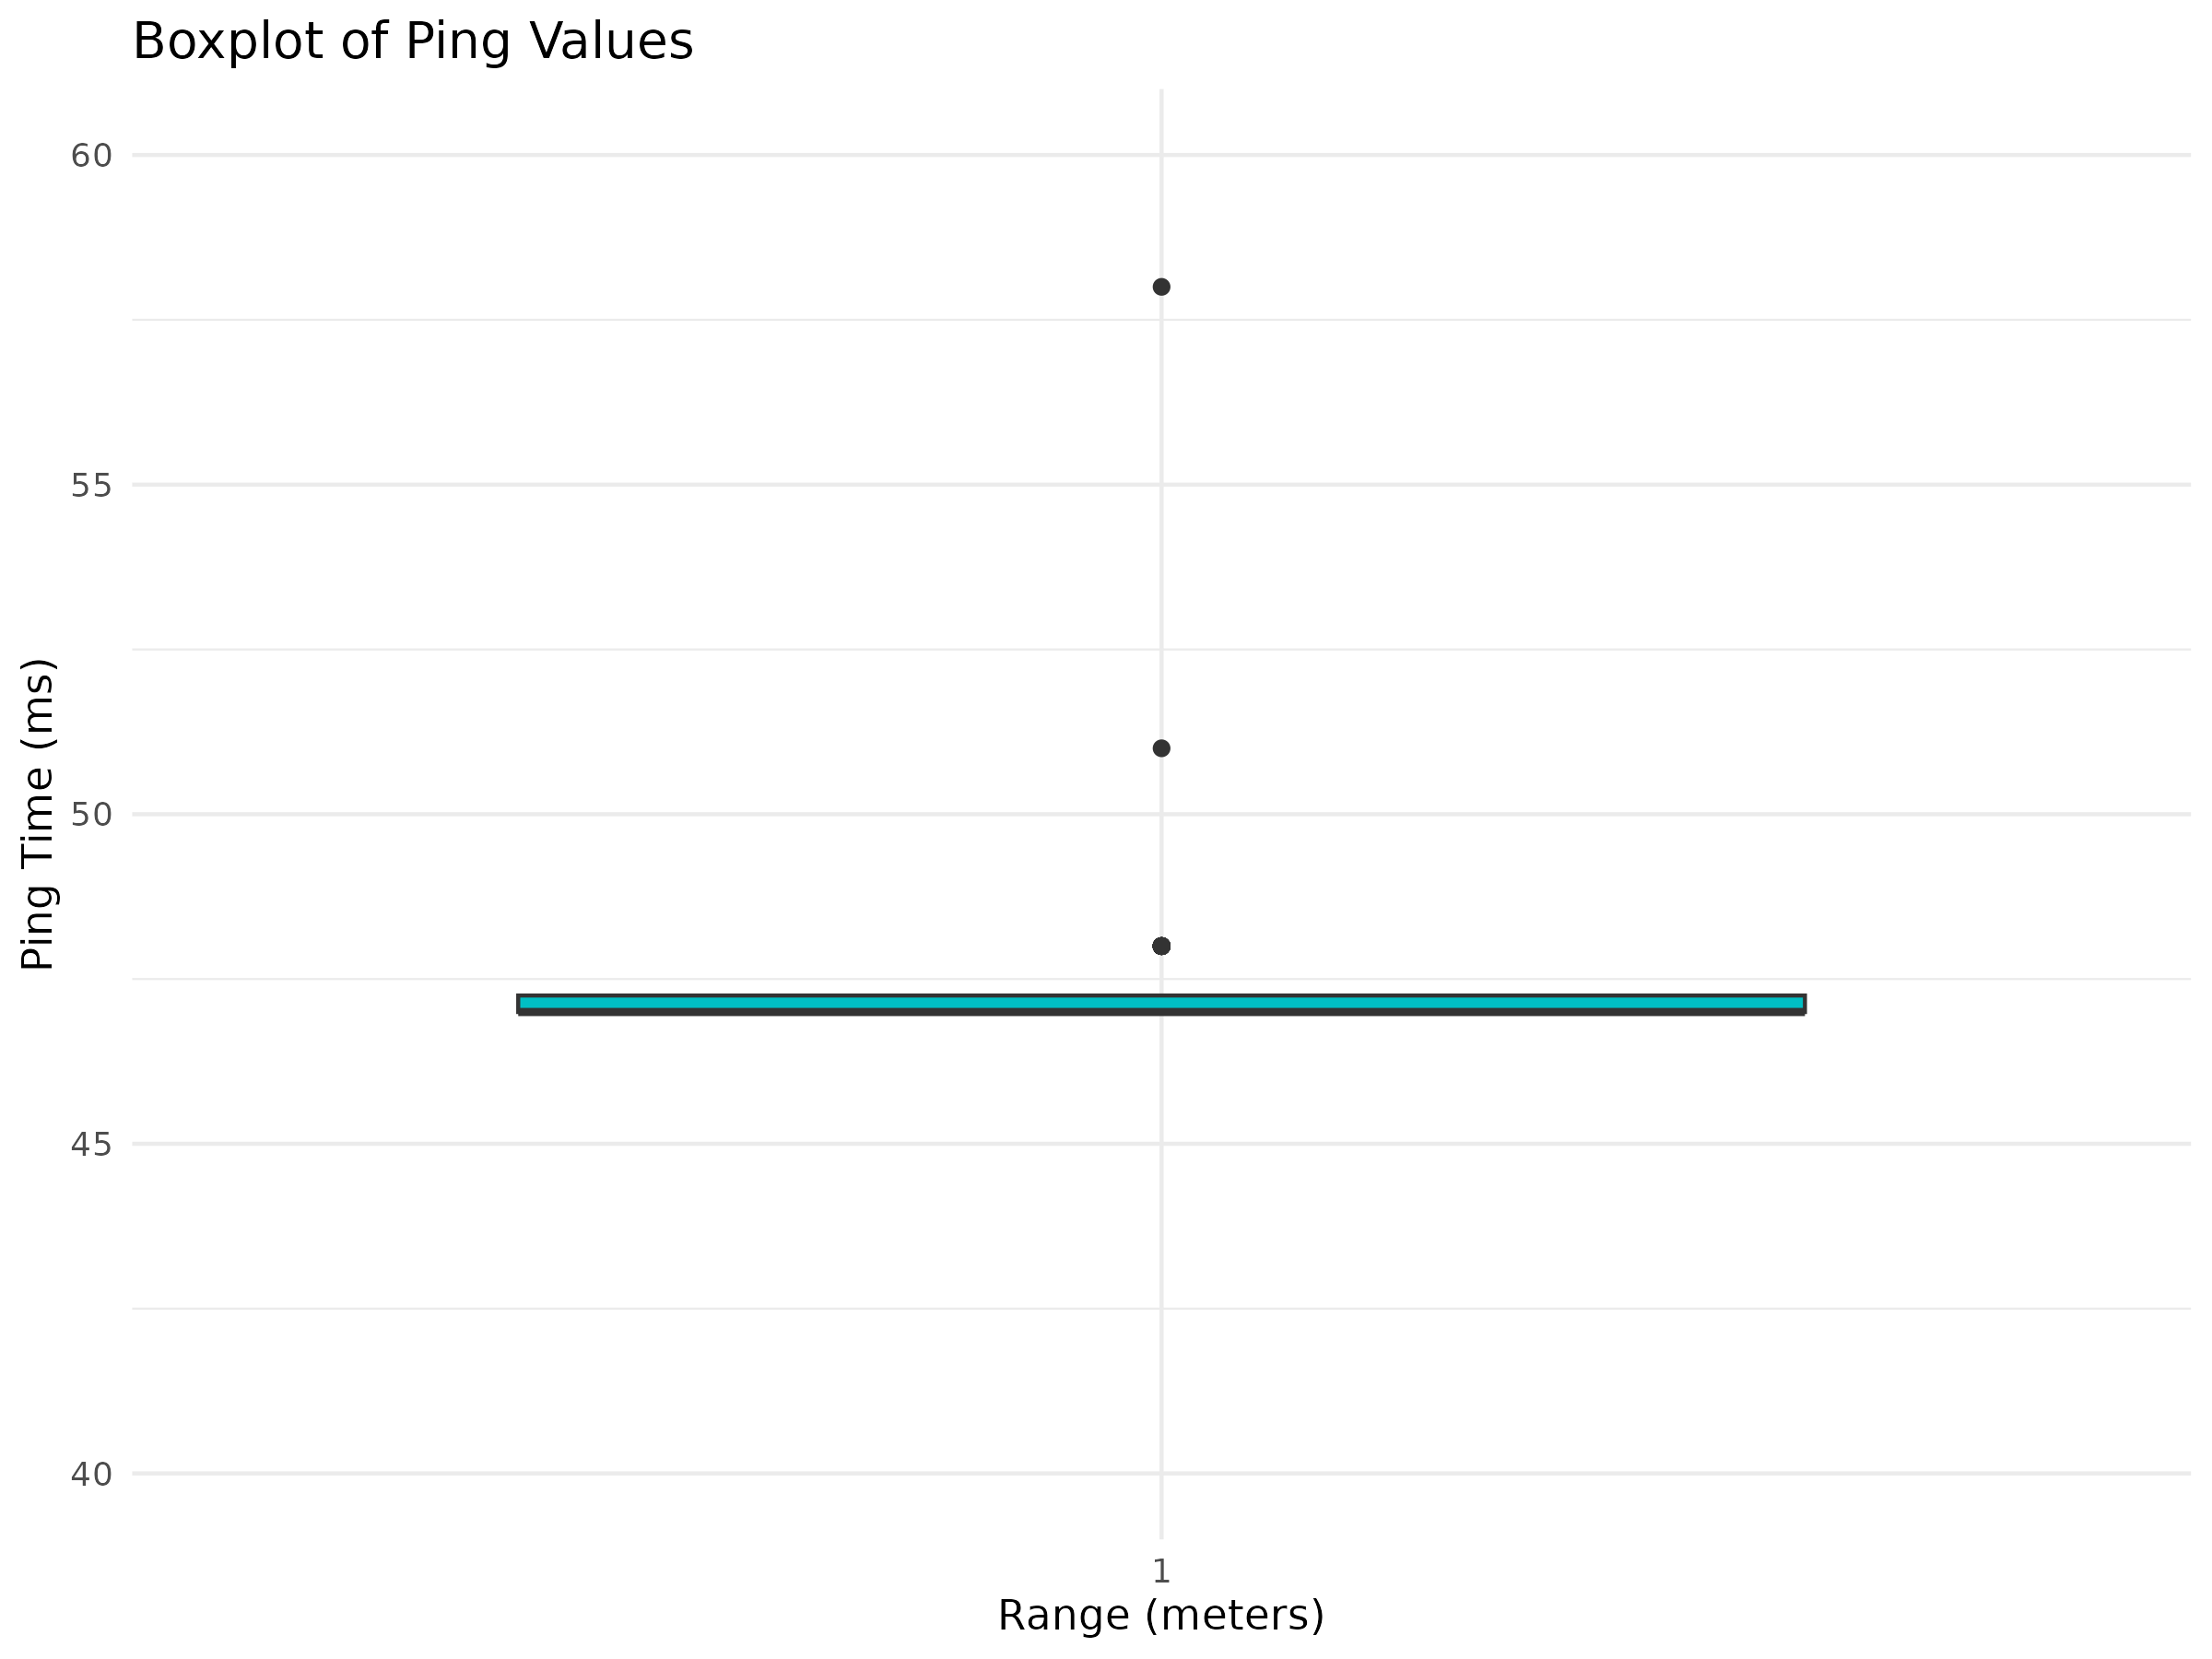
\includegraphics[width=.45\textwidth]{rstudio/analysis/plots/ping_net_ping.png}
     \vspace{\ftspace}
     \caption{Ping response time using two ESP32C3s with the Networking Library and SSP Add-on Library}
     \label{fig:net_ping}
 \end{figure}

A ping test using the Networking Library and the SSP Add-on Library was conducted at a fixed range of one meter. The test was only performed at a fixed range, given the lack of variance in ping response time observed in Section \ref{sec:res_rssi} for various ranges. This was done for the purpose of comparison with the ping response time achieved by the test code used for the tests discussed in Section \ref{sec:res_rssi} and Section \ref{sec:res_angle}. The average value of the ping response time is approximately twice as high ($47.38\ ms$) compared to the values observed using the basic ESP-NOW code ($23.29\ ms$ and $20.04-20.14\ ms$ respectively). This is likely due to increased processing demands and the necessity to add the peer's MAC address to the ESP-NOW peer buffer before each transmission and remove it afterward. The ping time demonstrates a high degree of consistent, with a standard deviation of only $1.21\ ms$, as shown in Figure \ref{fig:net_ping} and Table \ref{tab:ping}. 
%However, it should be noted that there are some outliers present, as evidenced by the figures presented in the tables.

\begin{table}[H]
    \centering
    \begin{tabular}{|c|c|l|l|c|c|c|c|c|}
    \hline
        Range & Packet Loss & \multicolumn{2}{l|}{Measurement} & \multicolumn{5}{c|}{Values} \\\hline
        [meters] & [\%] & \multicolumn{2}{l|}{} & mean & std & min & max & median \\\hline\hline
        1 m & 0 & Ping & [ms] & 47.38 & 1.21 & 47 & 58 & 47 \\\hline
    \end{tabular}
    \vspace{\ftspace}
    \caption{Ping time and packet loss measurements using the Networking Library and SSP Add-on Library}
    \label{tab:ping}
\end{table}

Using base ESP-NOW with minimal code, with no interrupt handlers and no other additional code, such as to save values for analysis, which might slow processing speed, the minimum value for ping response time achieved at minimal range under optimal conditions was $4\ ms$.

\subsection{\label{sec:res_angle}Antenna Angle Effects on RSSI and Ping Response Time}

\begin{figure}[H]
    \centering
    \begin{subfigure}{0.45\textwidth}
        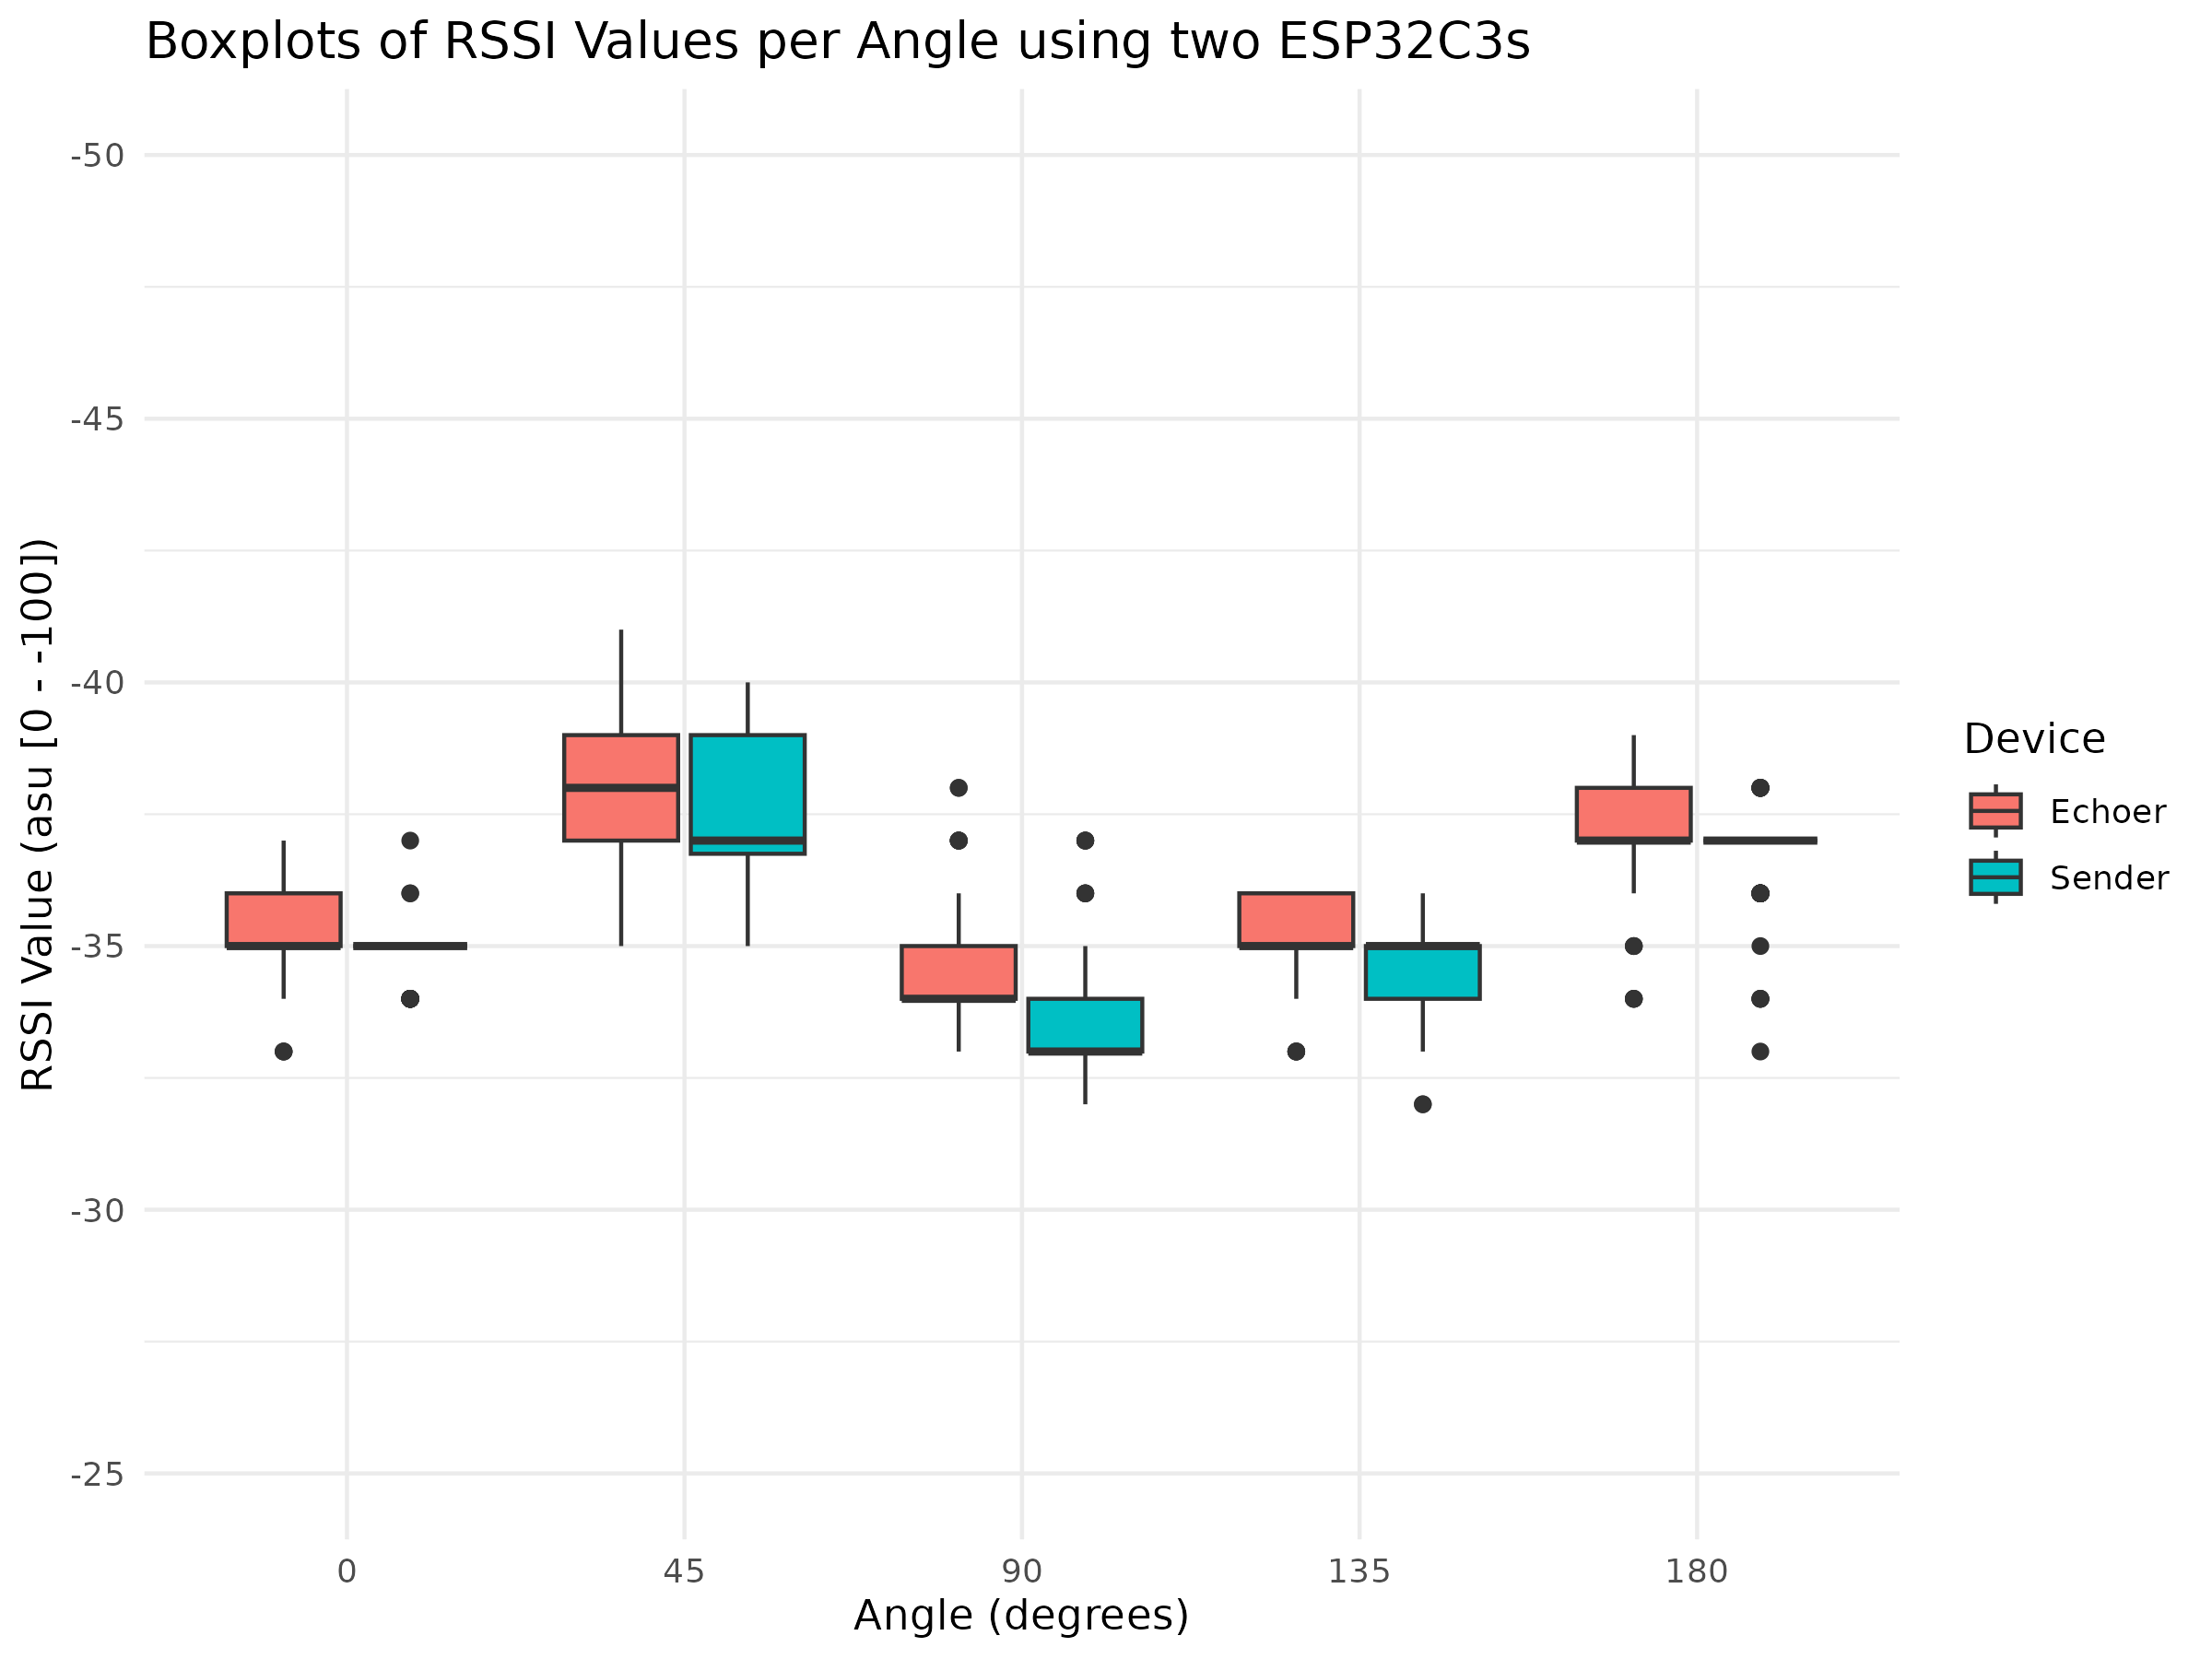
\includegraphics[width=\linewidth]{rstudio/analysis/plots/angle_rssi_box.png}
    \end{subfigure}
    % \begin{subfigure}{0.45\textwidth}
    %     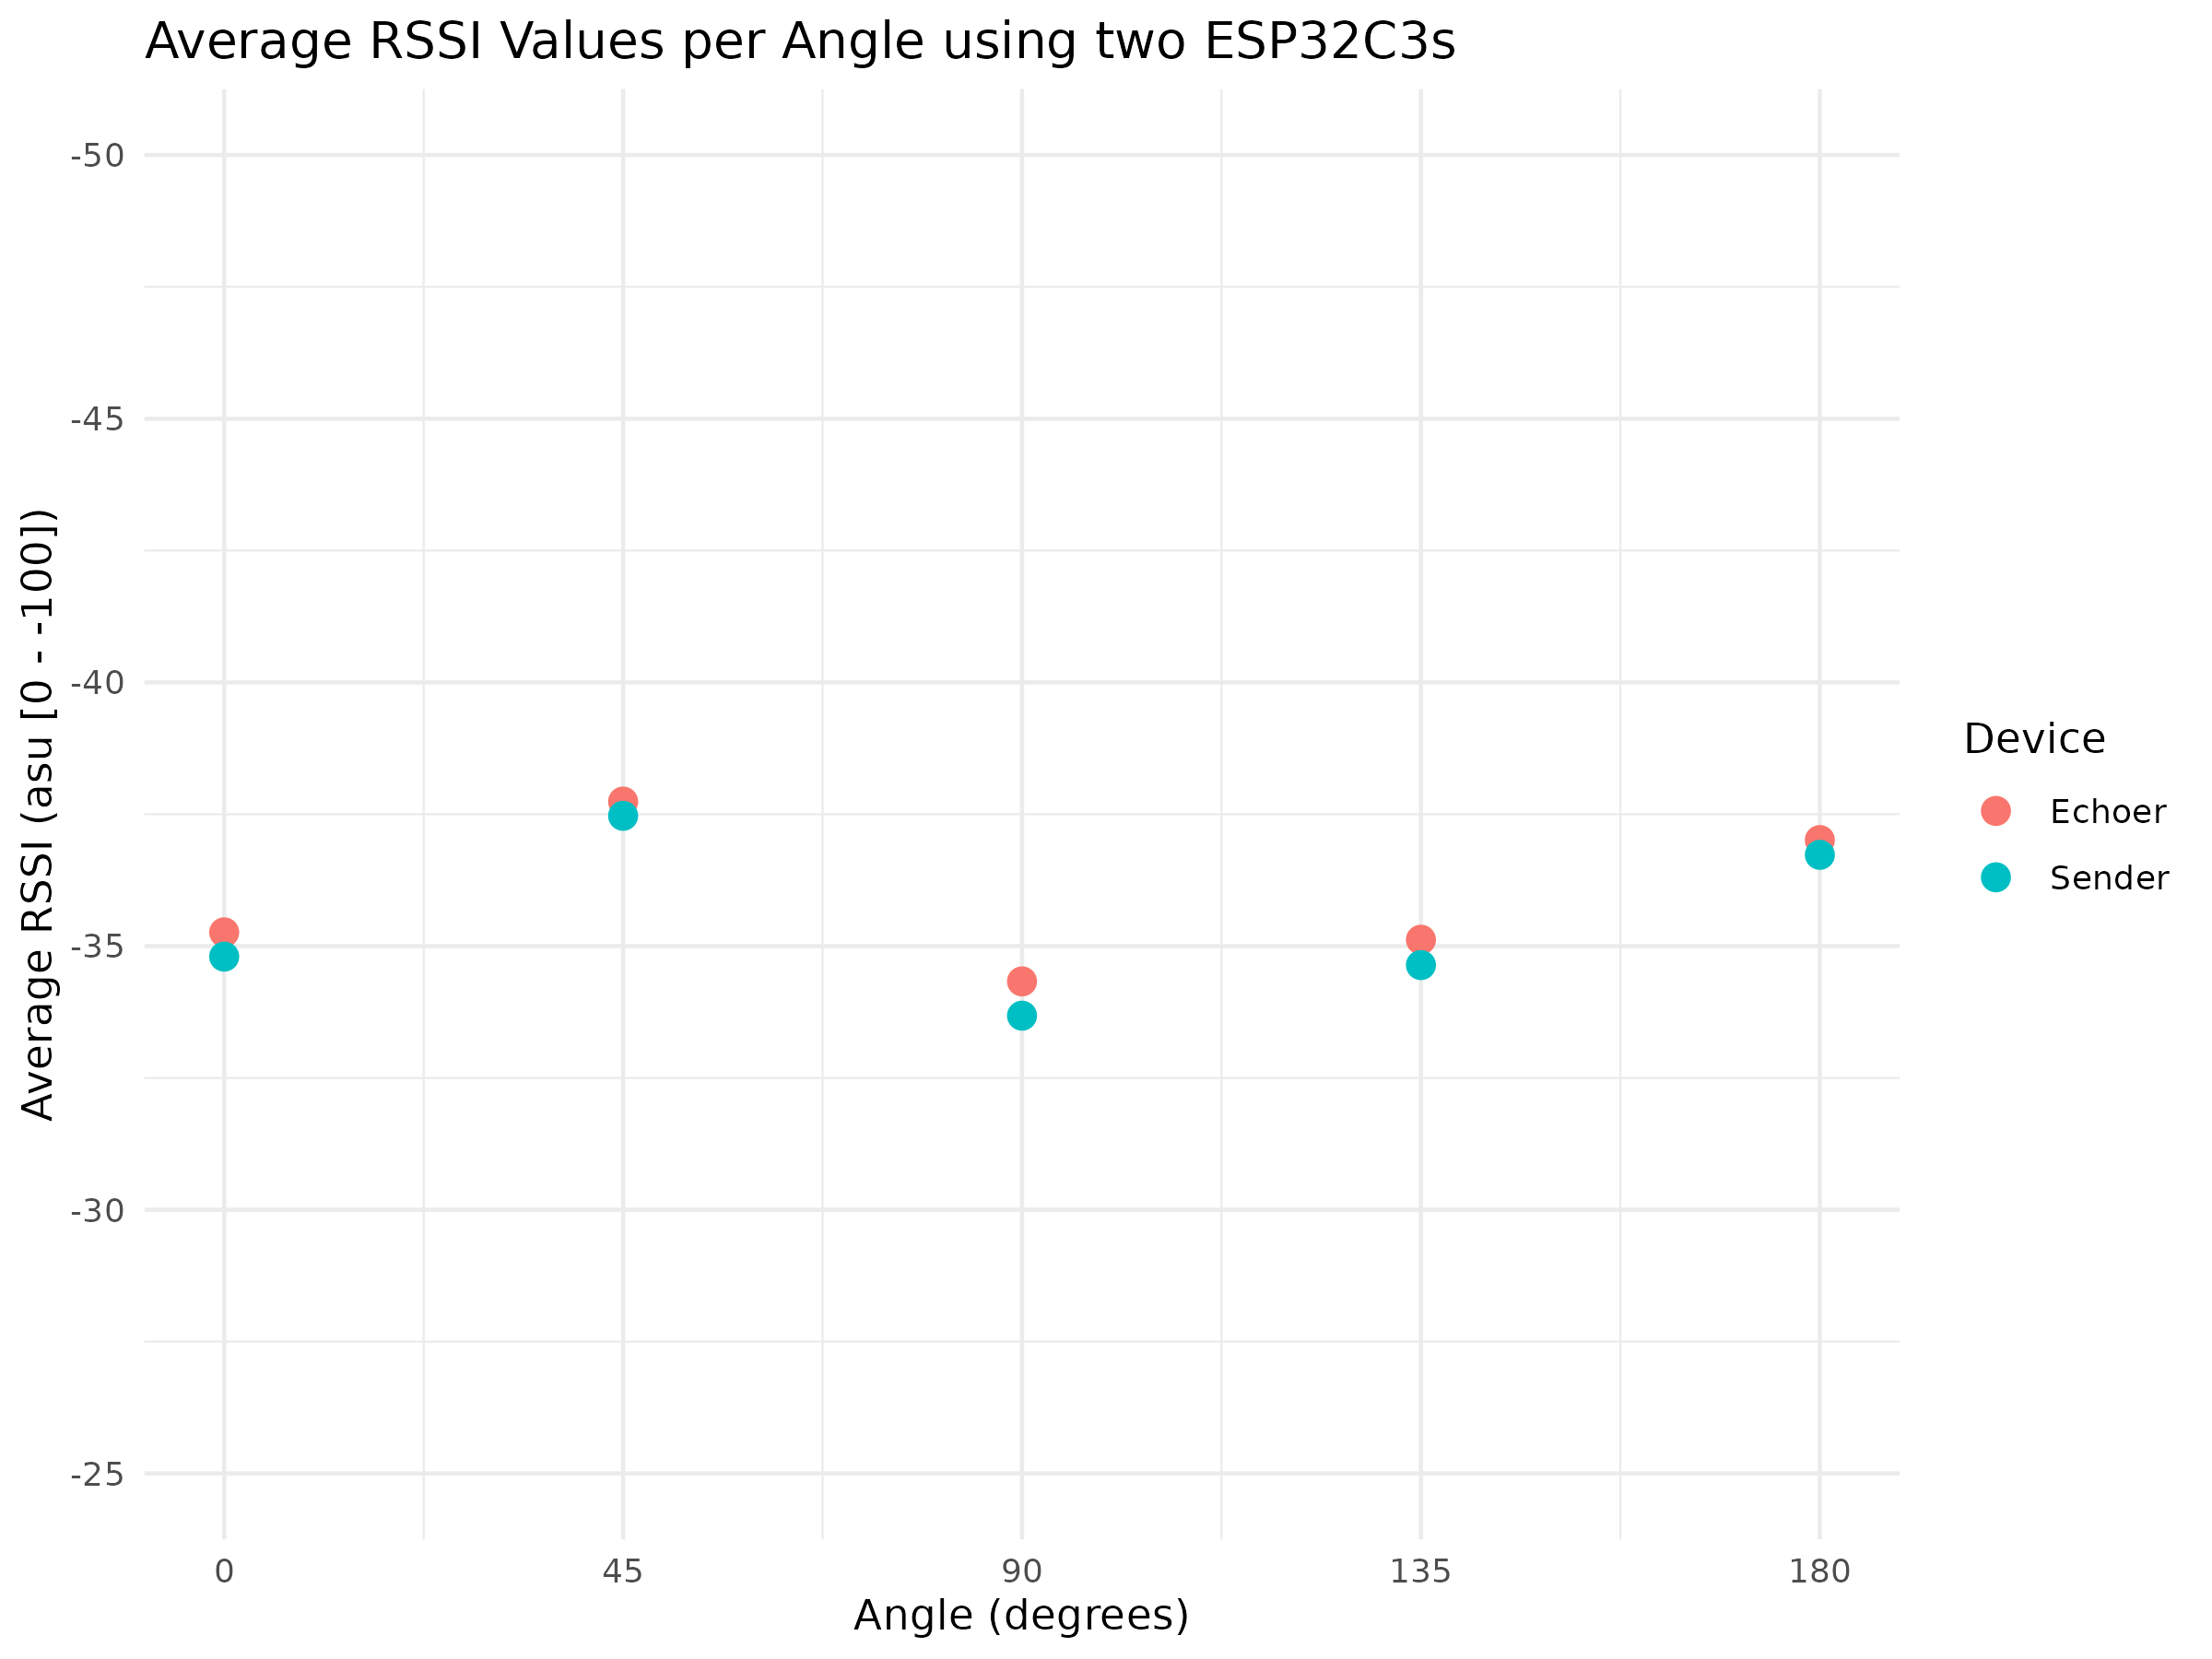
\includegraphics[width=\linewidth]{rstudio/analysis/plots/angle_avg_rssi.png}
    % \end{subfigure}
    \begin{subfigure}{0.45\textwidth}
        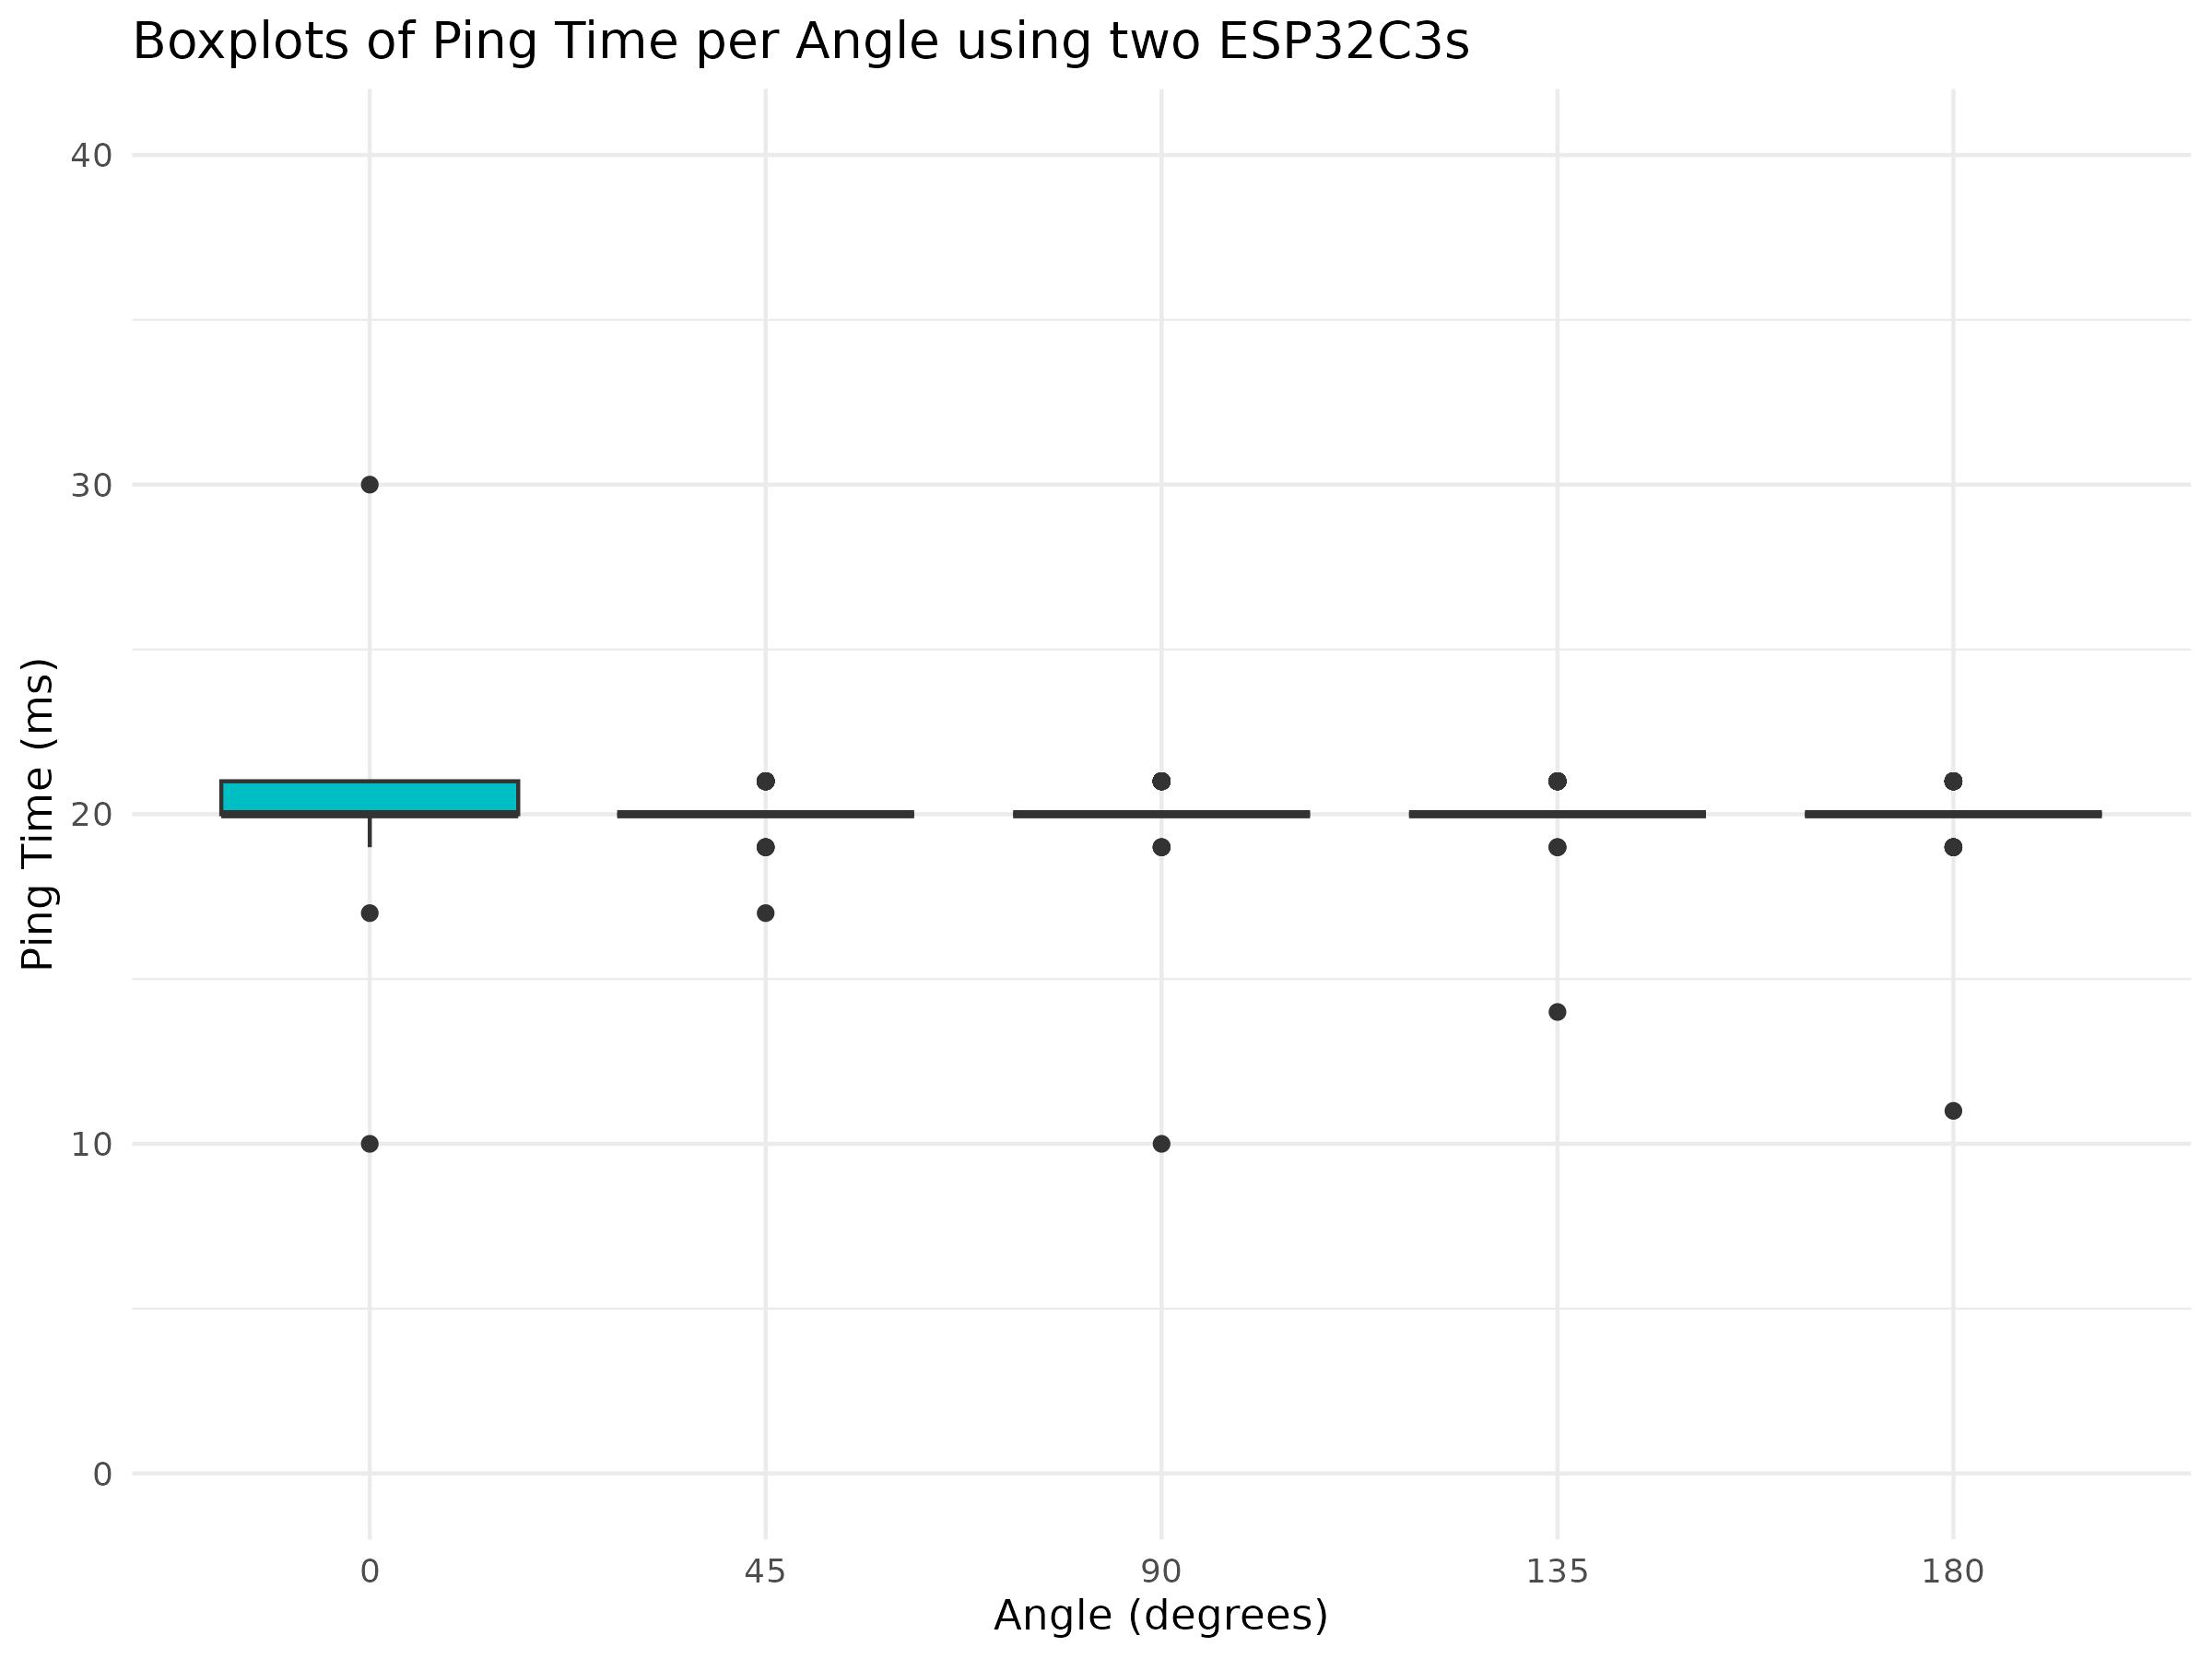
\includegraphics[width=\linewidth]{rstudio/analysis/plots/angle_ping_box.png}
    \end{subfigure}
    % \begin{subfigure}{0.45\textwidth}
    %     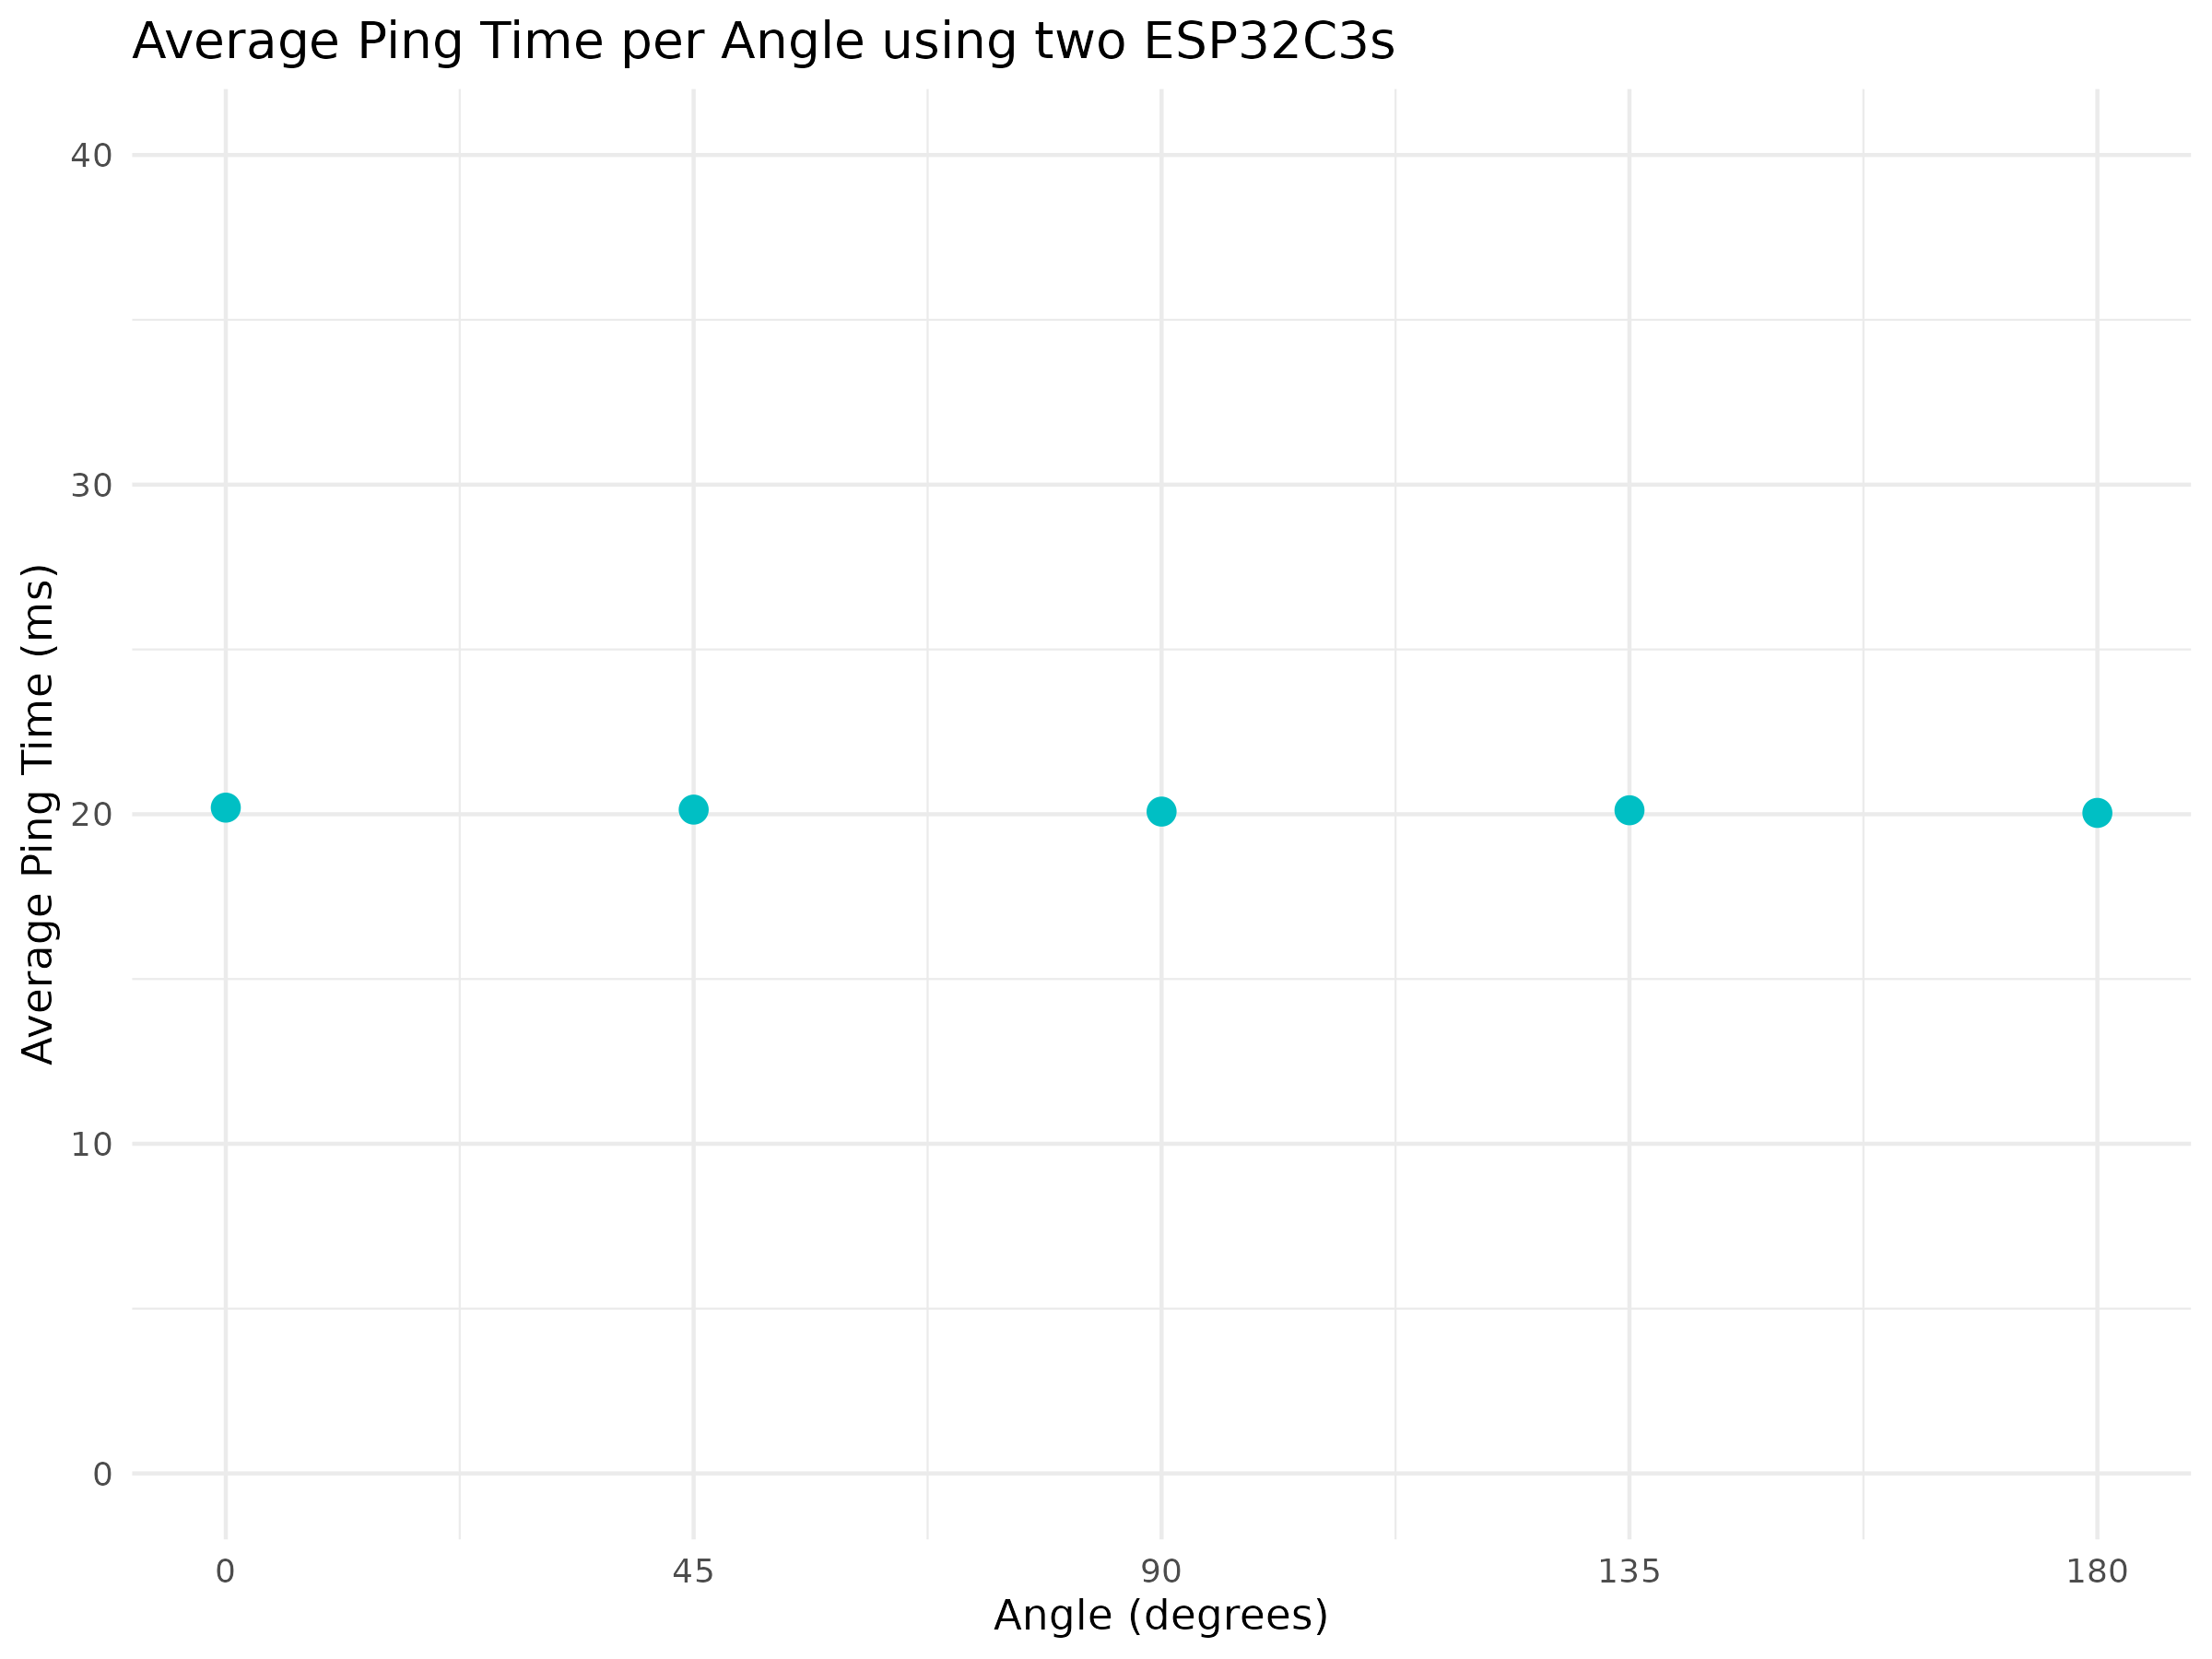
\includegraphics[width=\linewidth]{rstudio/analysis/plots/angle_avg_ping.png}
    % \end{subfigure}
    \vspace{\ftspace}
    \caption{RSSI and ping response time depending on antenna angle}
    \label{fig:antennaangle}
\end{figure}

\begin{table}[H]
    \centering
    \begin{tabular}{|c|c|l|l|c|c|c|c|c|}
    \hline
        Angle & Packet Loss & \multicolumn{2}{l|}{Measurement} & \multicolumn{5}{c|}{Values} \\\hline
        [\degree] & [\%] & \multicolumn{2}{l|}{} & mean & std & min & max & median \\\hline\hline
        \multirow{3}{*}{$0\degree$} & \multirow{1}{*}{0} & RSSI 1 & [asu] & -35.71 & 0.6 & -37 & -35 & -36 \\\cline{2-9}%\cline{2-9}
        %&& Time 1 &  &  &  &  &  \\\cline{2-9}\cline{2-9}
        & \multirow{2}{*}{0} & RSSI 2 & [asu] & -34.8 & 0.51 & -37 & -35 & -35 \\\cline{3-9}
        %&& Time 2 &  &  &  &  &  \\\cline{3-9}
        && Ping & [ms] & 20.2 & 1.53 & 10 & 30 & 20 \\\hline\hline
        \multirow{3}{*}{$45\degree$} & \multirow{1}{*}{0} & RSSI 1 & [asu] & -37.74 & 1.47 & -41 & -35 & 38 \\\cline{2-9}%\cline{2-9}
        %&& Time 1 &  &  &  &  &  \\\cline{2-9}\cline{2-9}
        & \multirow{2}{*}{0} & RSSI 2 & [asu] & -37.47 &1.49 & -40 & -35 & -37 \\\cline{3-9}
        %&& Time 2 &  &  &  &  &  \\\cline{3-9}
        && Ping & [ms] & 20.14 & 0.58 & 17 & 21 & 20 \\\hline\hline
        \multirow{3}{*}{$90\degree$} & \multirow{1}{*}{0} & RSSI 1 & [asu] & -34.33 & 1.18 & -38 & -33 & -34 \\\cline{2-9}%\cline{2-9}
        %&& Time 1 &  &  &  &  &  \\\cline{2-9}\cline{2-9}
        & \multirow{2}{*}{0} & RSSI 2 & [asu] & -33.68 & 1.15 & -37 & -32 & -33 \\\cline{3-9}
        %&& Time 2 &  &  &  &  &  \\\cline{3-9}
        && Ping & [ms] & 20.08 & 1.12 & 10 & 21 & 20 \\\hline\hline
        \multirow{3}{*}{$135\degree$} & \multirow{1}{*}{0} & RSSI 1 & [asu] & -35.12 & 0.72 & -36 & -33 & -35 \\\cline{2-9}%\cline{2-9}
        %&& Time 1 &  &  &  &  &  \\\cline{2-9}\cline{2-9}
        & \multirow{2}{*}{0} & RSSI 2 & [asu] & -34.64 & 0.7 & -36 & -32 & -35 \\\cline{3-9}
        %&& Time 2 &  &  &  &  &  \\\cline{3-9}
        && Ping & [ms] & 20.12 & 0.77 & 14 & 21 & 20 \\\hline\hline
        \multirow{3}{*}{$180\degree$} & \multirow{1}{*}{0} & RSSI 1 & [asu] & -37.01 & 0.96 & -39 & -34 & -37 \\\cline{2-9}%\cline{2-9}
        %&& Time 1 &  &  &  &  &  \\\cline{2-9}\cline{2-9}
        & \multirow{2}{*}{0} & RSSI 2 & [asu] & -36.73 & 0.86 & -39 & -33 & -37 \\\cline{3-9}
        %&& Time 2 &  &  &  &  &  \\\cline{3-9}
        && Ping & [ms] & 20.04 & 1.05 & 11 & 21 & 20 \\\hline
    \end{tabular}
    \vspace{\ftspace}
    \caption{RSSI, ping response time and packet loss measurements depending on antenna angle}
    \label{tab:angle_res}
\end{table}

This test was conducted on the basis of anecdotal observations from the Smart Playground project, as described in Section \ref{sec:methods_test_net}, which suspects that device and antenna orientation might affect RSSI values. As illustrated in Figure \ref{fig:antennaangle}, the ping time values remain largely consistent. While there is some slight variation in RSSI values, these are likely normal RSSI value fluctuations that were observed between different measurements, and therefore appear to be independent of the orientation of the MCBs and their antenna.

\subsection{\label{sec:res_battery}Power Consumption and Battery Endurance}

As outlined in Section \ref{sec:methods_test_net}, the endurance of the battery of devices was tested. With a fully charged LiPo battery, the device was able to broadcast messages every second for a duration of a slightly over $4.5\ hours$ ($16313723\ ms$) in the first test using a $3.7\ V\  350\ mAh$ battery. In the two subsequent tests, a slightly extended runtime of approximately $5\ hours$ ($18186793\ ms$ and $18135873\ ms$) using a $3.7\ V\  420\ mAh$ battery was achieved. %After this the device ran out of battery crashed, and while it managed to start up again a few times to send a couple more messages it eventually died completely.

\subsection{\label{sec:res_reliability}Reliability}
A reliability test was conducted during the first Hackathon, the methodology of which is detailed in Section \ref{sec:methods_hackathon1} and the results of which are discussed in Section \ref{sec:res_hackathon1}. As part of this test, 18 participants used a Dahal Board running the \textit{boop-o-meter} program to send messages to each other. The program kept track and count of the amount of messages sent and received, with the objective being to achieve 999 received and sent messages. During the test, no issues with transmission or reliability of the Networking Library or ESP-NOW were observed. However, given the high volume of messages and their peer-to-peer nature, it was not possible to track and validate every single message. The code used for this usability test, can be found in Appendix \hyperref[chap:apx_e]{E}.

\subsection{\label{sec:res_limitations}Limitations}

As outlined in the above results, the Networking Library is subject to certain limitations. One such limitation is inherent to the peer-to-peer connectionless networking model, in which no connection is established, with the system merely transmitting the message, akin to a radio station, with the notable distinction that the messages are directed to specific recipients. While the Networking Library does include a test for successful transmission based on the built-in ESP-NOW receipt confirmation, currently the Library only attempts to resend the message for a total of three attempts without any further failure handling. This is a deliberate choice to minimise the complexity of the Networking approach, but a limitation nonetheless and can result in messages being lost during transmission, as discussed in Section \ref{sec:res_rssi}. While the transmission of messages using the library is reliable, there are circumstances and scenarios where this might be inhibited. Hence, in scenarios in which reliable message delivery is essential, the Networking Library might not be able to deliver the required reliability. \\

A further limitation of the Networking Library is the increased processing time in comparison to the transmission time. Specifically, the Networking Library requires approximately $47\ ms$ for a ping, whereas the fastest back-and-forth transmission achieved using ESP-NOW with MicroPython firmware was $4\ ms$. This discrepancy illustrates a limitations of MicroPython, particularly its speed and memory constraints. However, it also highlights the potential of the technology if it were to be optimised and written in a lower-level language such as C++, which could enhance its efficiency in a resource-constrained environment such as the MCB. This inefficiency can hinder scalability and responsiveness for larger and more complex projects. This represents the trade-off between optimisation, feature richness and accessibility.\\

During testing, particularly the RSSI, ping response time and packet loss measurement test using two ESP32C6 MCBs, issues were encountered. These tests revealed challenges in achieving a transmission distances greater than 15 meters using two ESP32C6 MCBs, which could be indicative of  inconsistencies in the underlying hardware or network transmission performance that could affect overall reliability of the system. These issues, however, were not observed with the ESP32C3, which could transmit up to a maximum range of 240 meters, with reliable transmission possible up to 50 meters, at which point packet loss became an issue. \\

The development process further revealed some issues with the underlying ESP-NOW implementation for MicroPython. Once the Networking Library had become sufficiently complex, unknown Wi-Fi errors and memory errors were encountered, in addition to errors with Thonny and its interaction with ESP32-based MCBs. The unknown Wi-Fi error, in particular, proved to be a significant challenge in the troubleshooting process, further complicated by the fact that once this error occurred, the initialisation of the networking was no longer possible, necessitating the re-flashing of the firmware onto the MCB. While some reports of this error were available online, they provided no definitive solution. Through rigorous debugging, a cause was identified, with the length of the Networking Library files being the primary factor. It was observed that the error manifested itself once the library exceeded approximately 1000 lines in length. This finding has influenced the decision to divide the library into two parts: the Networking Library and the SSP Add-on Library. Following this decision, no further issues were encountered.

\section{\label{sec:res_capabilities}Smart System Platform} %reference to methods

In order to validate the design of the Smart System Platform and to support the core networking capability, certain parts of the platform were developed as a proof of concept, as well as used and validated during the second Hackathon, which is discussed in Section \ref{sec:res_hackathon2}. The various developed parts are presented in this section.

\subsection{\label{sec:res_design}Platform and Framework Design} %reference to methods

\begin{figure}[H]
    \centering
    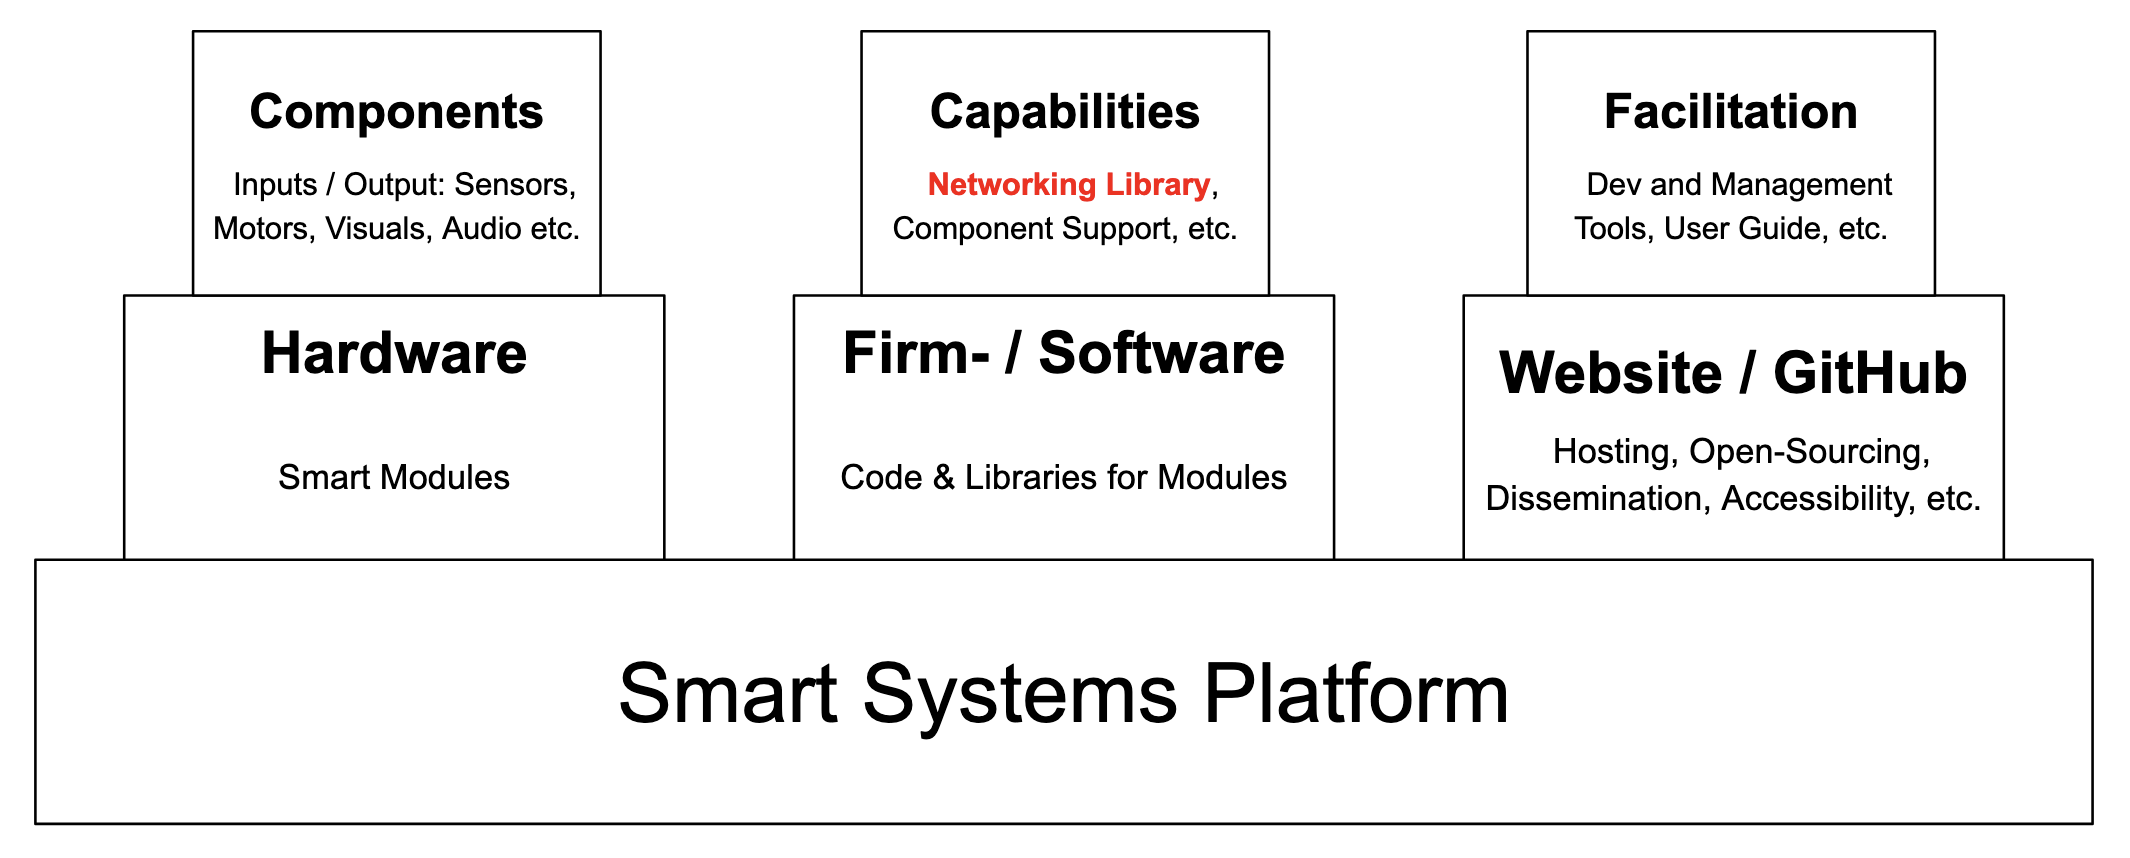
\includegraphics[width=\linewidth]{overleaf/images/SSP.png}
    \vspace{\ftspace}
    \caption{Simplified Smart System Platform architecture}
    \label{fig:ssp_architecture}
\end{figure}

In response to the second research question, which sought to ascertain methods for enhancing usability and accessibility of the developed networking capability for an educational robotics system such as the Smart Motors, the Smart System Platform was designed and partially developed. The platform is a basic framework, centred around the networking capability and is designed to be usable as a platform for the creation and development of network-enabled educational robotics projects. \\

The design of the Smart System Platform is outlined in Section \ref{sec:methods_ssp_des} and depicted in a simplified version in Figure \ref{fig:ssp_architecture}, is divided into three parts:
\begin{itemize}
    \item Hardware:\\
    This component encompasses the supported hardware, designated modules, which can be any MCB based on an ESP3 SoC running MicroPython firmware. It also includes the supported components, inputs and outputs, such as sensors and motors. The support is primarily based on the design of the Dahal board, which is the central component of the Smart Motors. 
    \item Software:\\
    This component is situated at the core of the platform and includes the various capabilities that the platform has been designed around and to enable, namely the Networking Library. The software part also includes various libraries and components for component support. 
    \item Documentation and Development:\\
    The third part of the platform is concerned with documentation and development, and includes the various tools and resources necessary to support the accessibility of the main parts of the platform, mainly its software, its use and its development. This third component includes the GitHub site, the central repository for any code or data related to the SSP project, a website that serves as an outreach platform and also as a base for hosting the various network development and management tools and user guides.
\end{itemize}

\subsection{\label{sec:res_website}Website}

\begin{figure}[H]
    \centering
    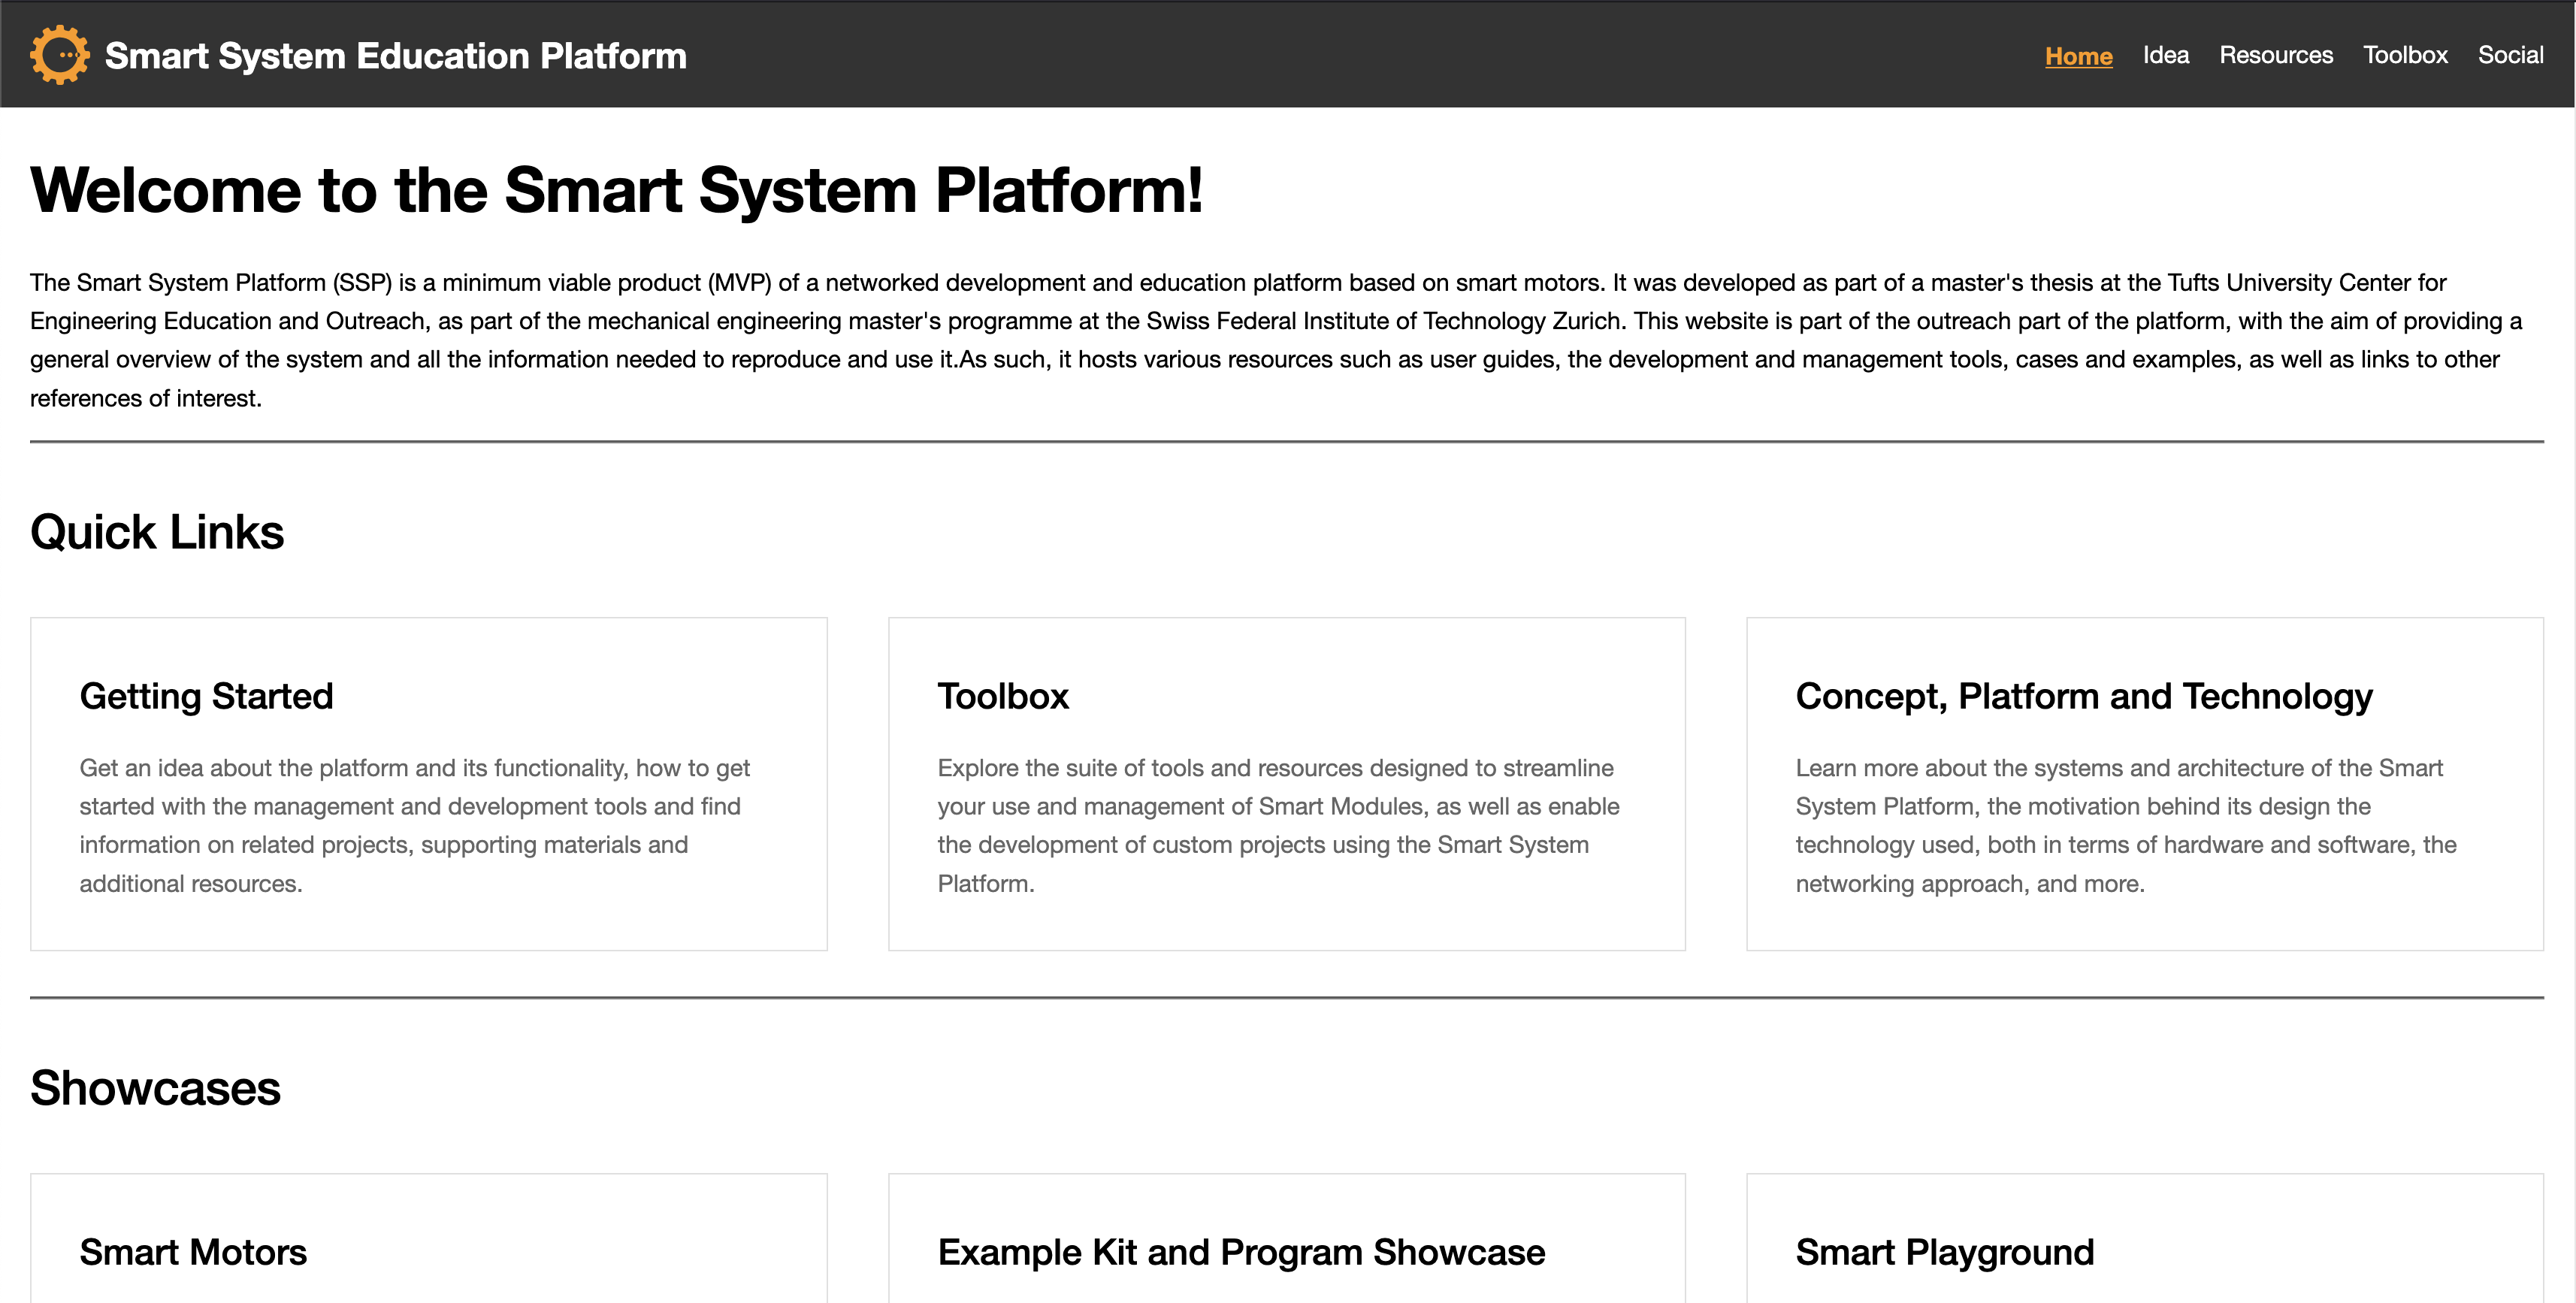
\includegraphics[width=\linewidth]{overleaf/images/website_landing_page.png}
    \vspace{\ftspace}
    \caption{Smart System Platform website landing page}
    \vspace{\ftspace}
    \label{fig:website_landing}
\end{figure}

The website consists of various pages, including an introduction page, information about the project and involved parties, as well as a user guide. It further hosts links to the various tools and provides background information on the concept of the Smart System Platform. The website's design aligns with the Swiss design style outlined in Section \ref{sec:methods_website}, as referenced by \citet{muller-brockmann_grid_2020, hollis_swiss_2006} in their work on the Swiss design style. The primary objective of the website's design is to ensure accessibility and the facilitate the effective dissemination of information. The website was tested using the Google for Developers PageSpeed Insights \citep{noauthor_pagespeed_nodate}, which resulted in an overall accessibility and usability score of 100 out of 100 for both mobile and desktop version of the webpage.

\begin{figure}[H]
    \centering
    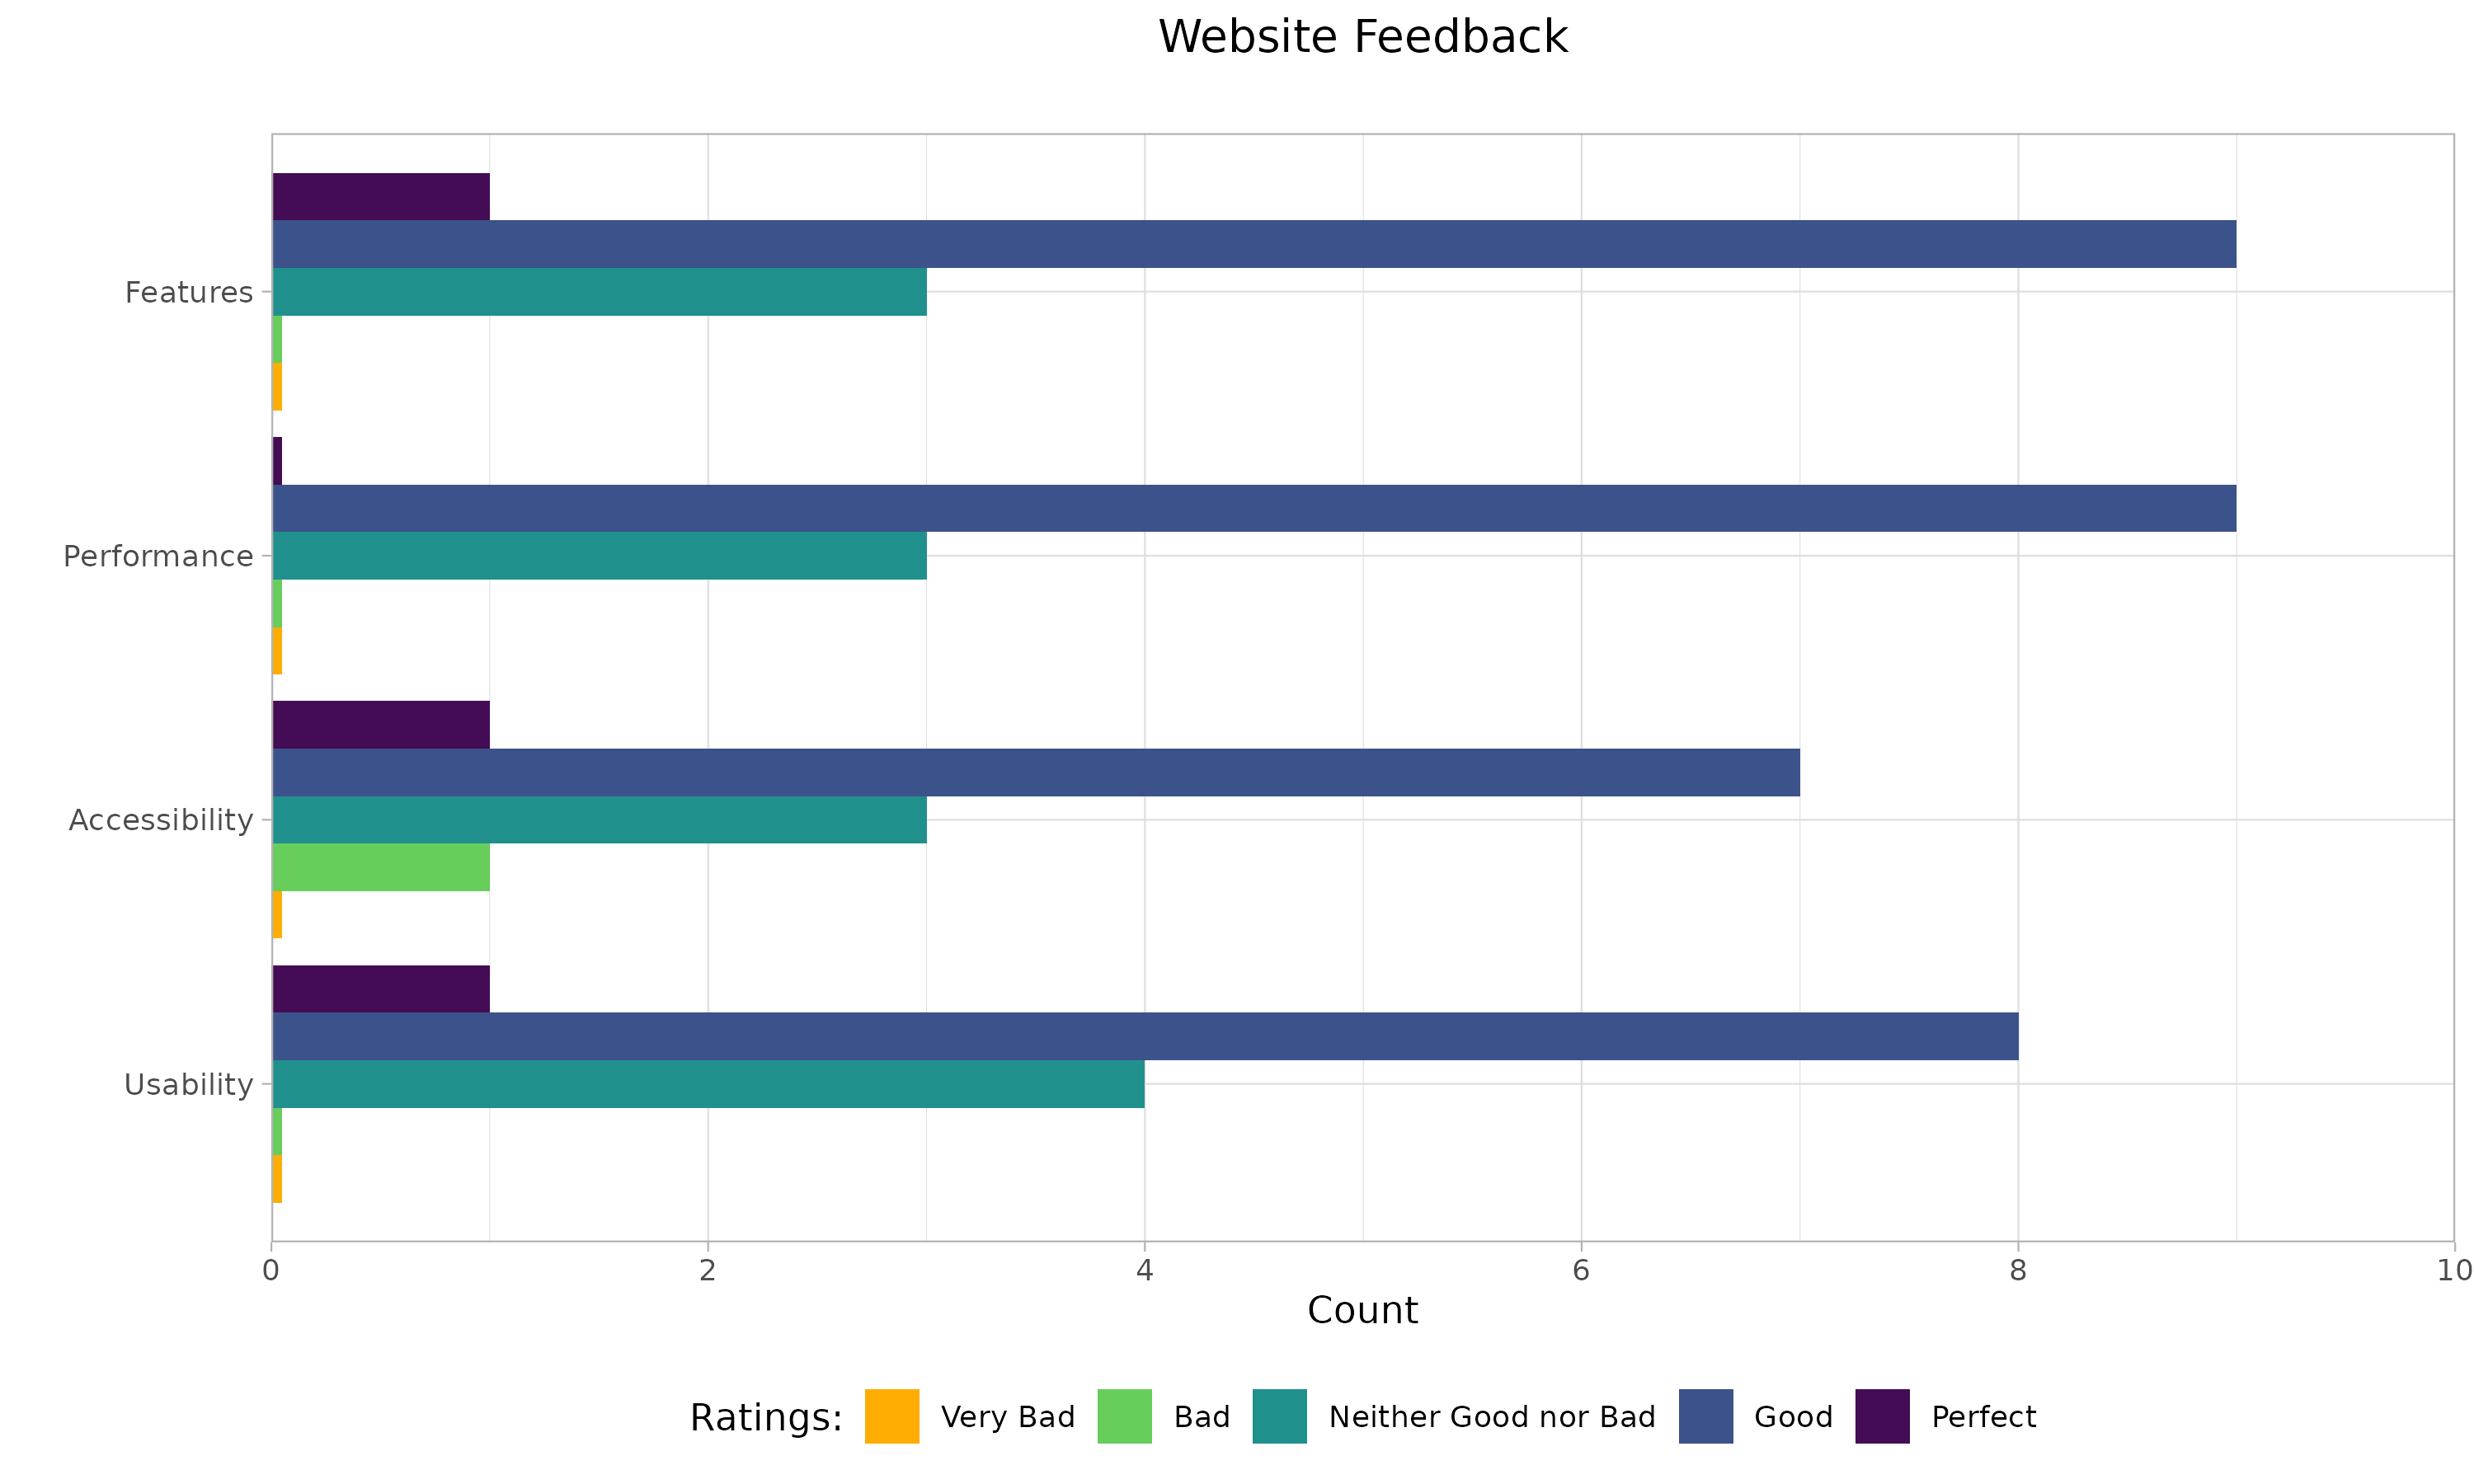
\includegraphics[width=.75\linewidth]{rstudio/survey/plots/website.png}
    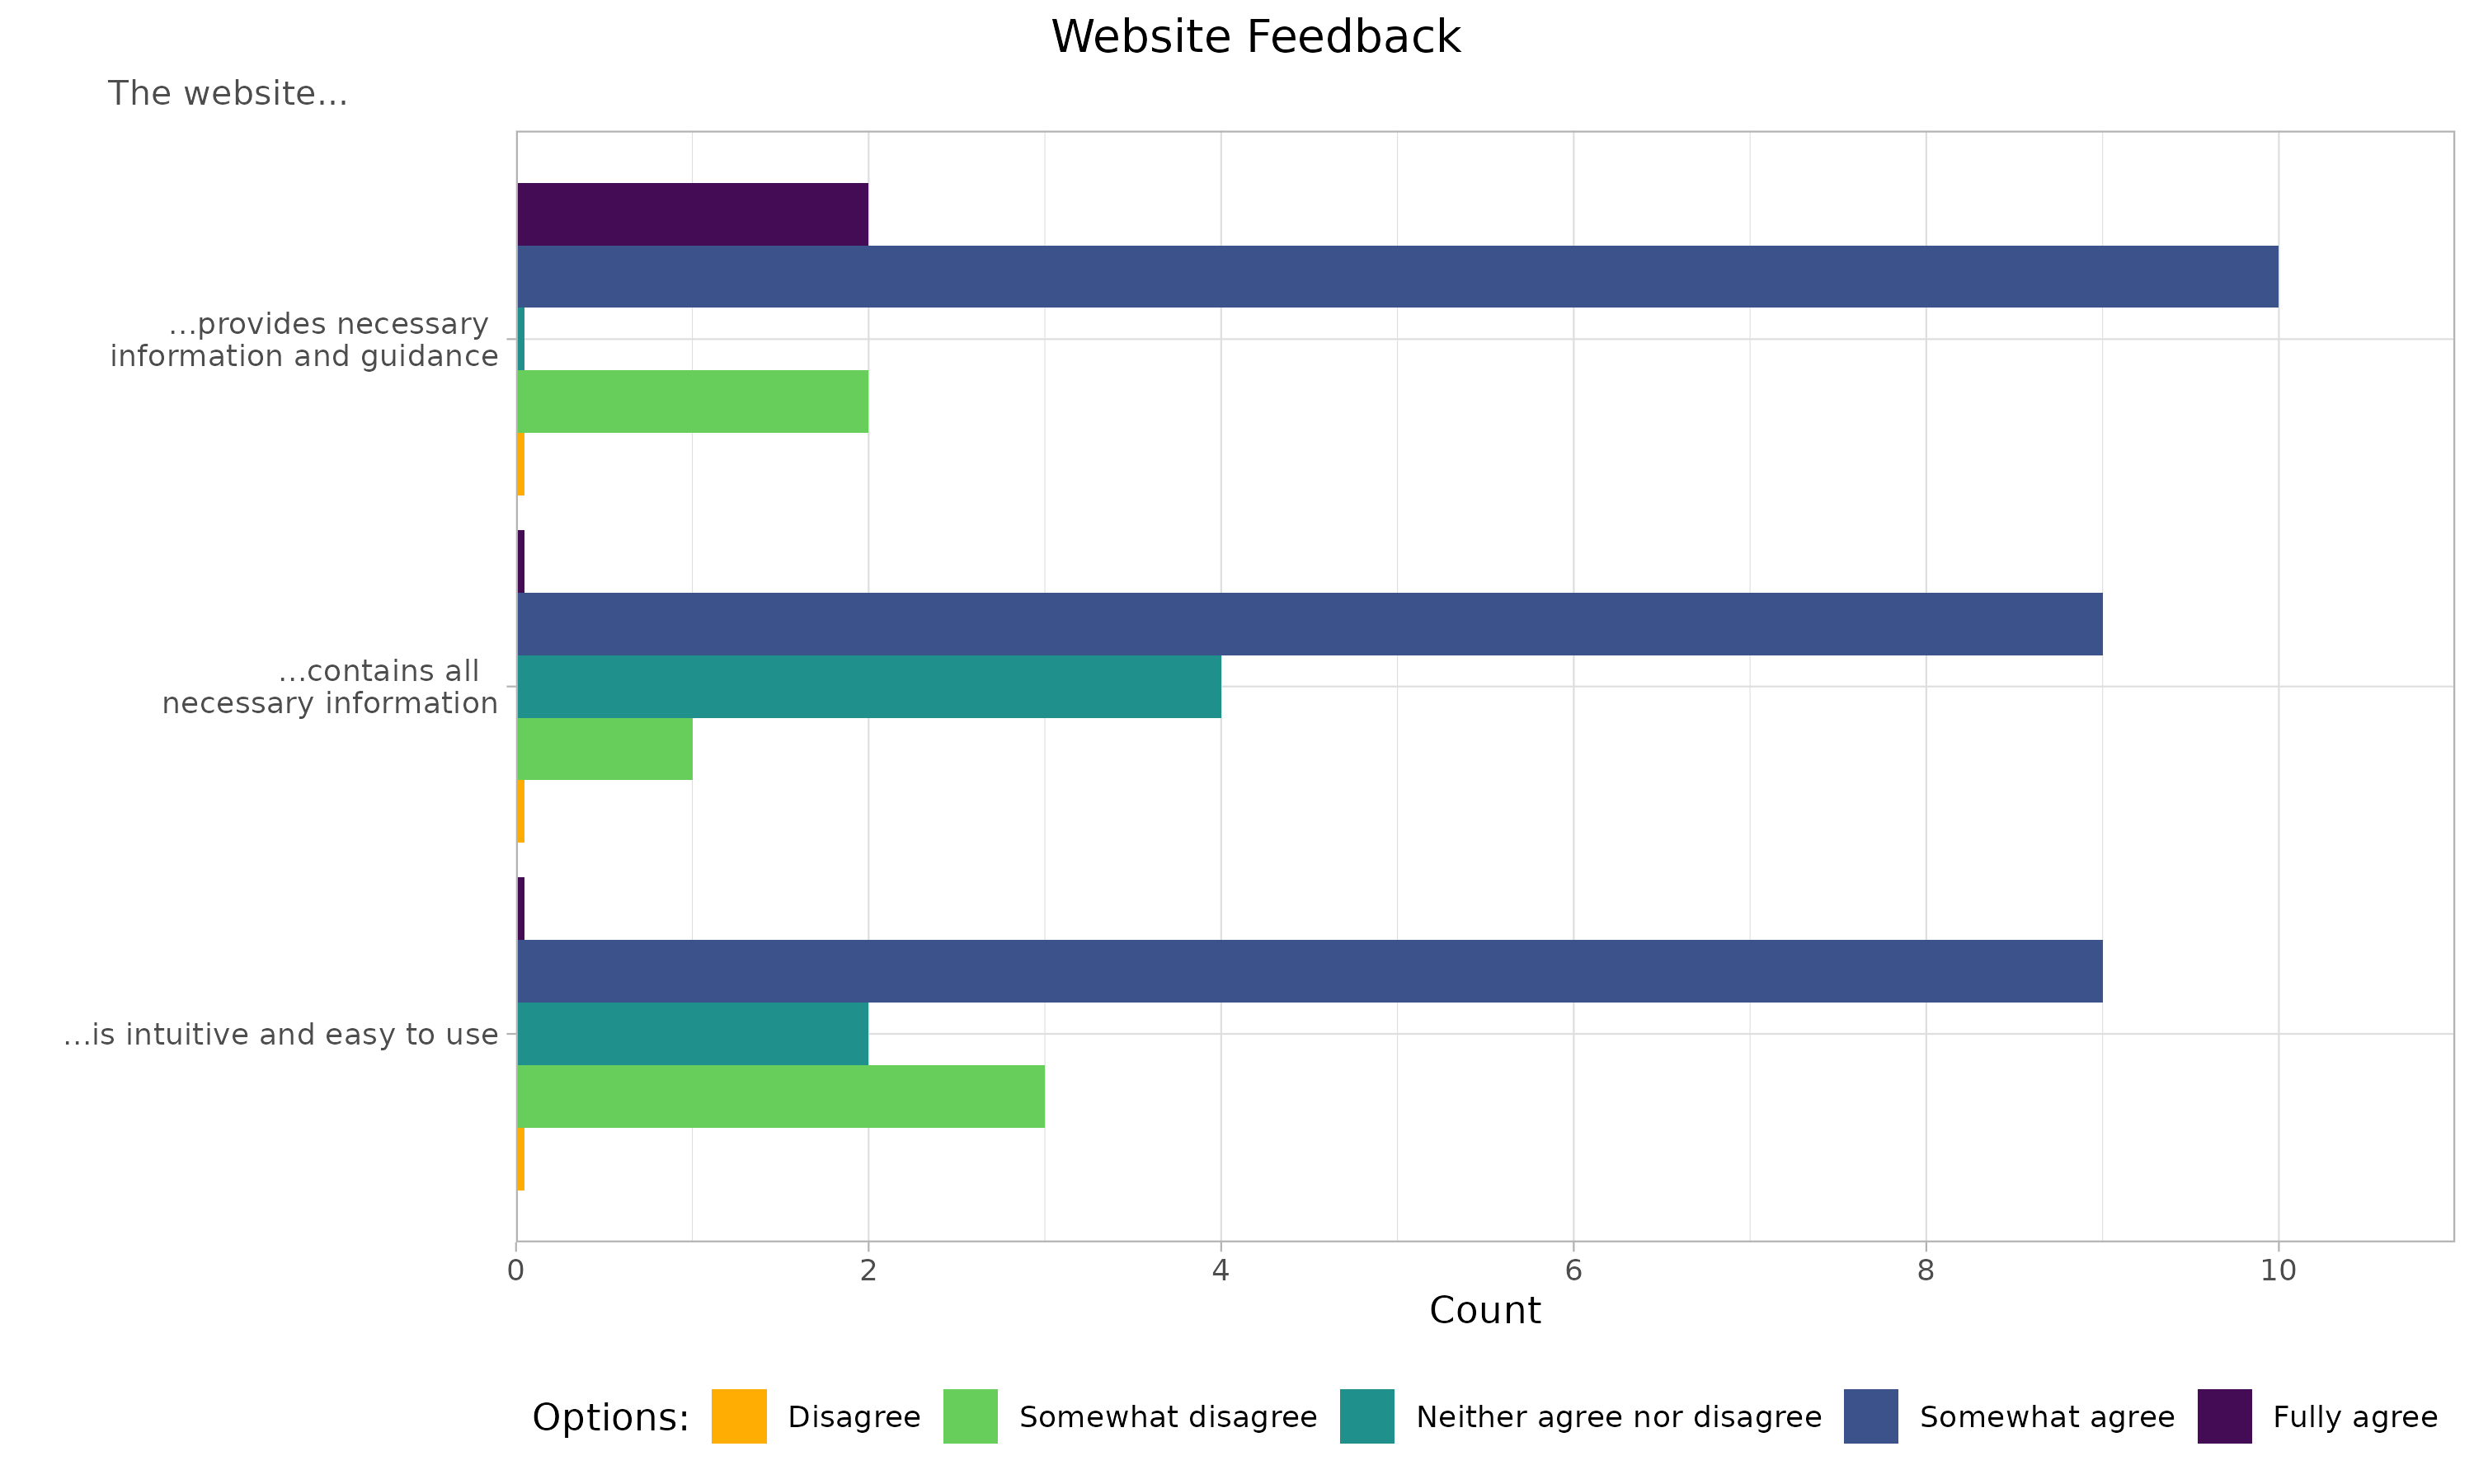
\includegraphics[width=.75\linewidth]{rstudio/survey/plots/website2.png}
    \vspace{\ftspace}
    \caption{Hackathon 2: Website questionnaire results}
    \vspace{\ftspace}
    \label{fig:website_questions}
\end{figure}

The ratings given to the website by the participants of Hackathon 2, shown in Figure \ref{fig:website_questions}, are predominantly positive, particularly with regard to content and features. Nevertheless, the ratings and the especially the individual comments suggest there are potential areas for enhancement, especially with regard to accessibility, the intuitiveness and the design of the website, as some technical difficulties and navigation issues were encountered by some users.

\subsection{\label{sec:res_tools}Development and Management Tools}

One of the website's and the Smart System Platform's main components, are the various networking development and management tools. The purpose of these tools is to facilitate the utilisation and advancement of the core networking functionality. The following section will thus examine and discuss these tools.

\subsubsection{\label{sec:res_ide}Integrated Development Environment}

\begin{figure}[H]
    \centering
    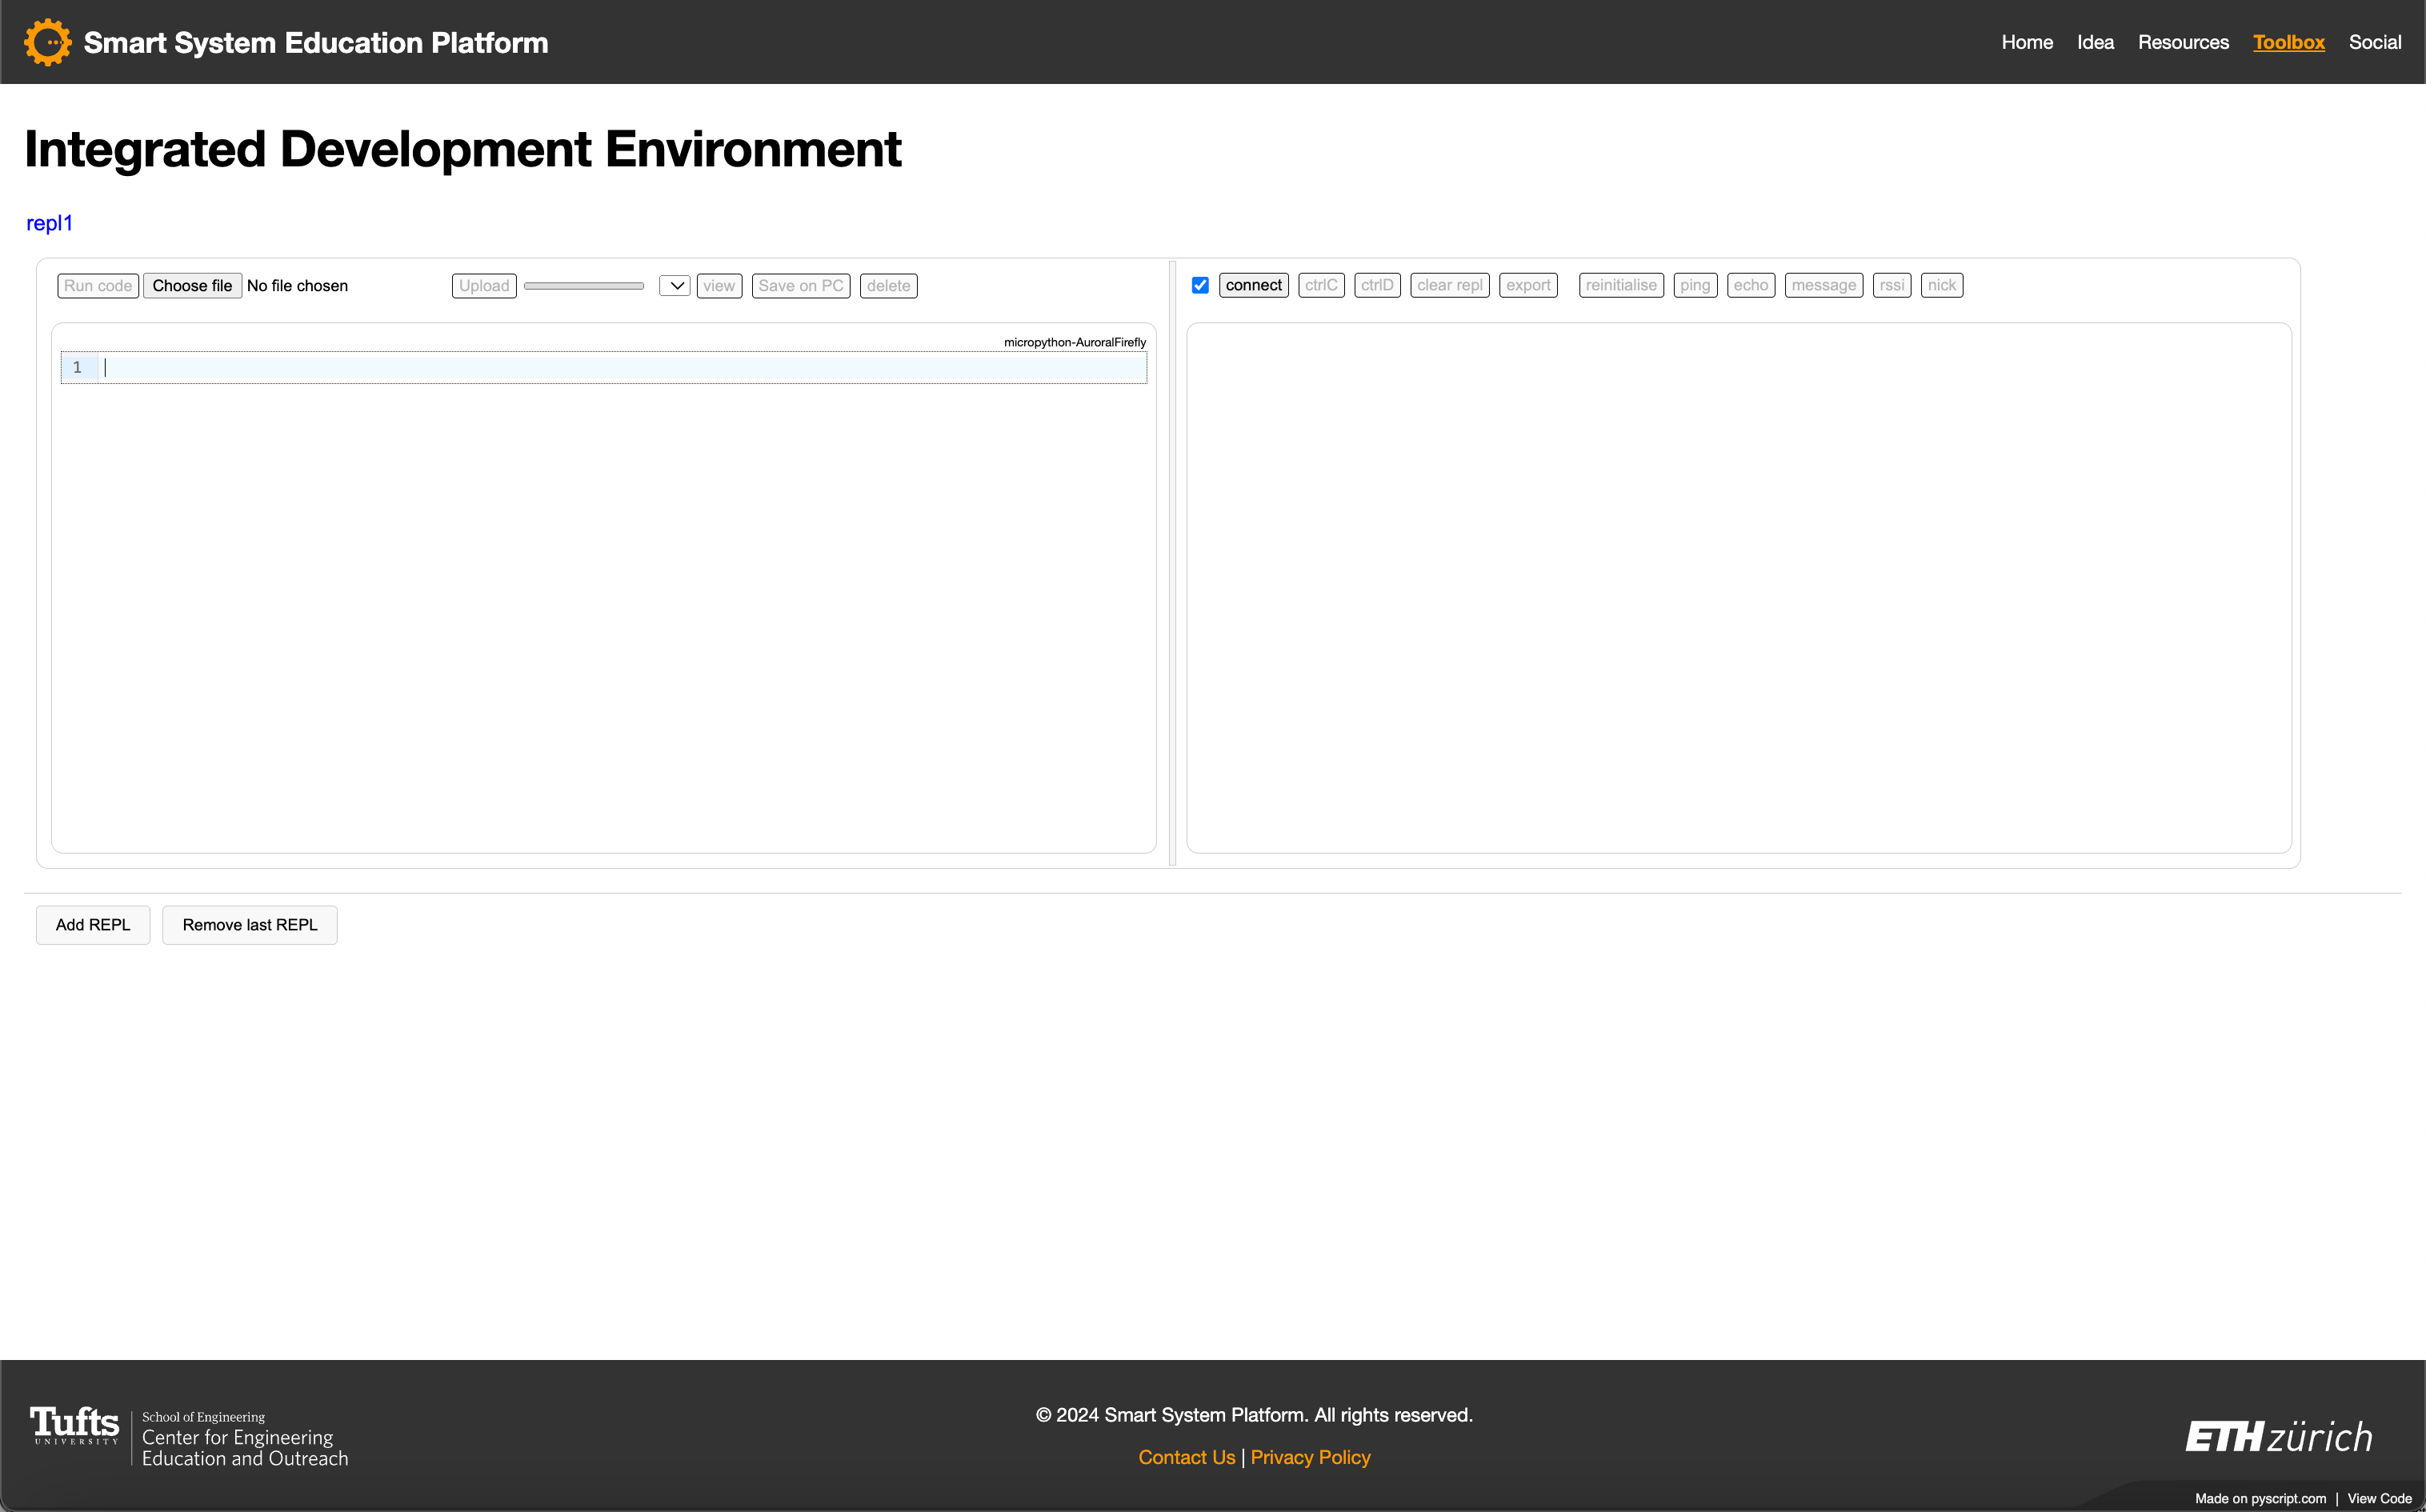
\includegraphics[width=\linewidth]{overleaf/images/ide_raw.png}
    \vspace{\ftspace}
    \caption{Custom Web IDE}
    \vspace{\ftspace}
    \label{fig:ide_raw}
\end{figure}

The custom Web-IDE was specifically developed for use with the Smart System Platform and the developed Networking Library, as described in Section \ref{sec:methods_ide}, and features a variety of custom features. The most notable feature being the multiple development tabs that can be added to the page. These tabs permit simultaneous development and REPL control of multiple devices, which is advantageous for networking development. Furthermore, the IDE facilitates the initiation of networking and the transmission of networking commands via pre-coded buttons within the REPL area. User feedback on the IDE has been largely positive, with suggestions for improvement relating to accessibility, intuitiveness and design, as well as performance, based on specific user feedback.

\begin{figure}[H]
    \centering
    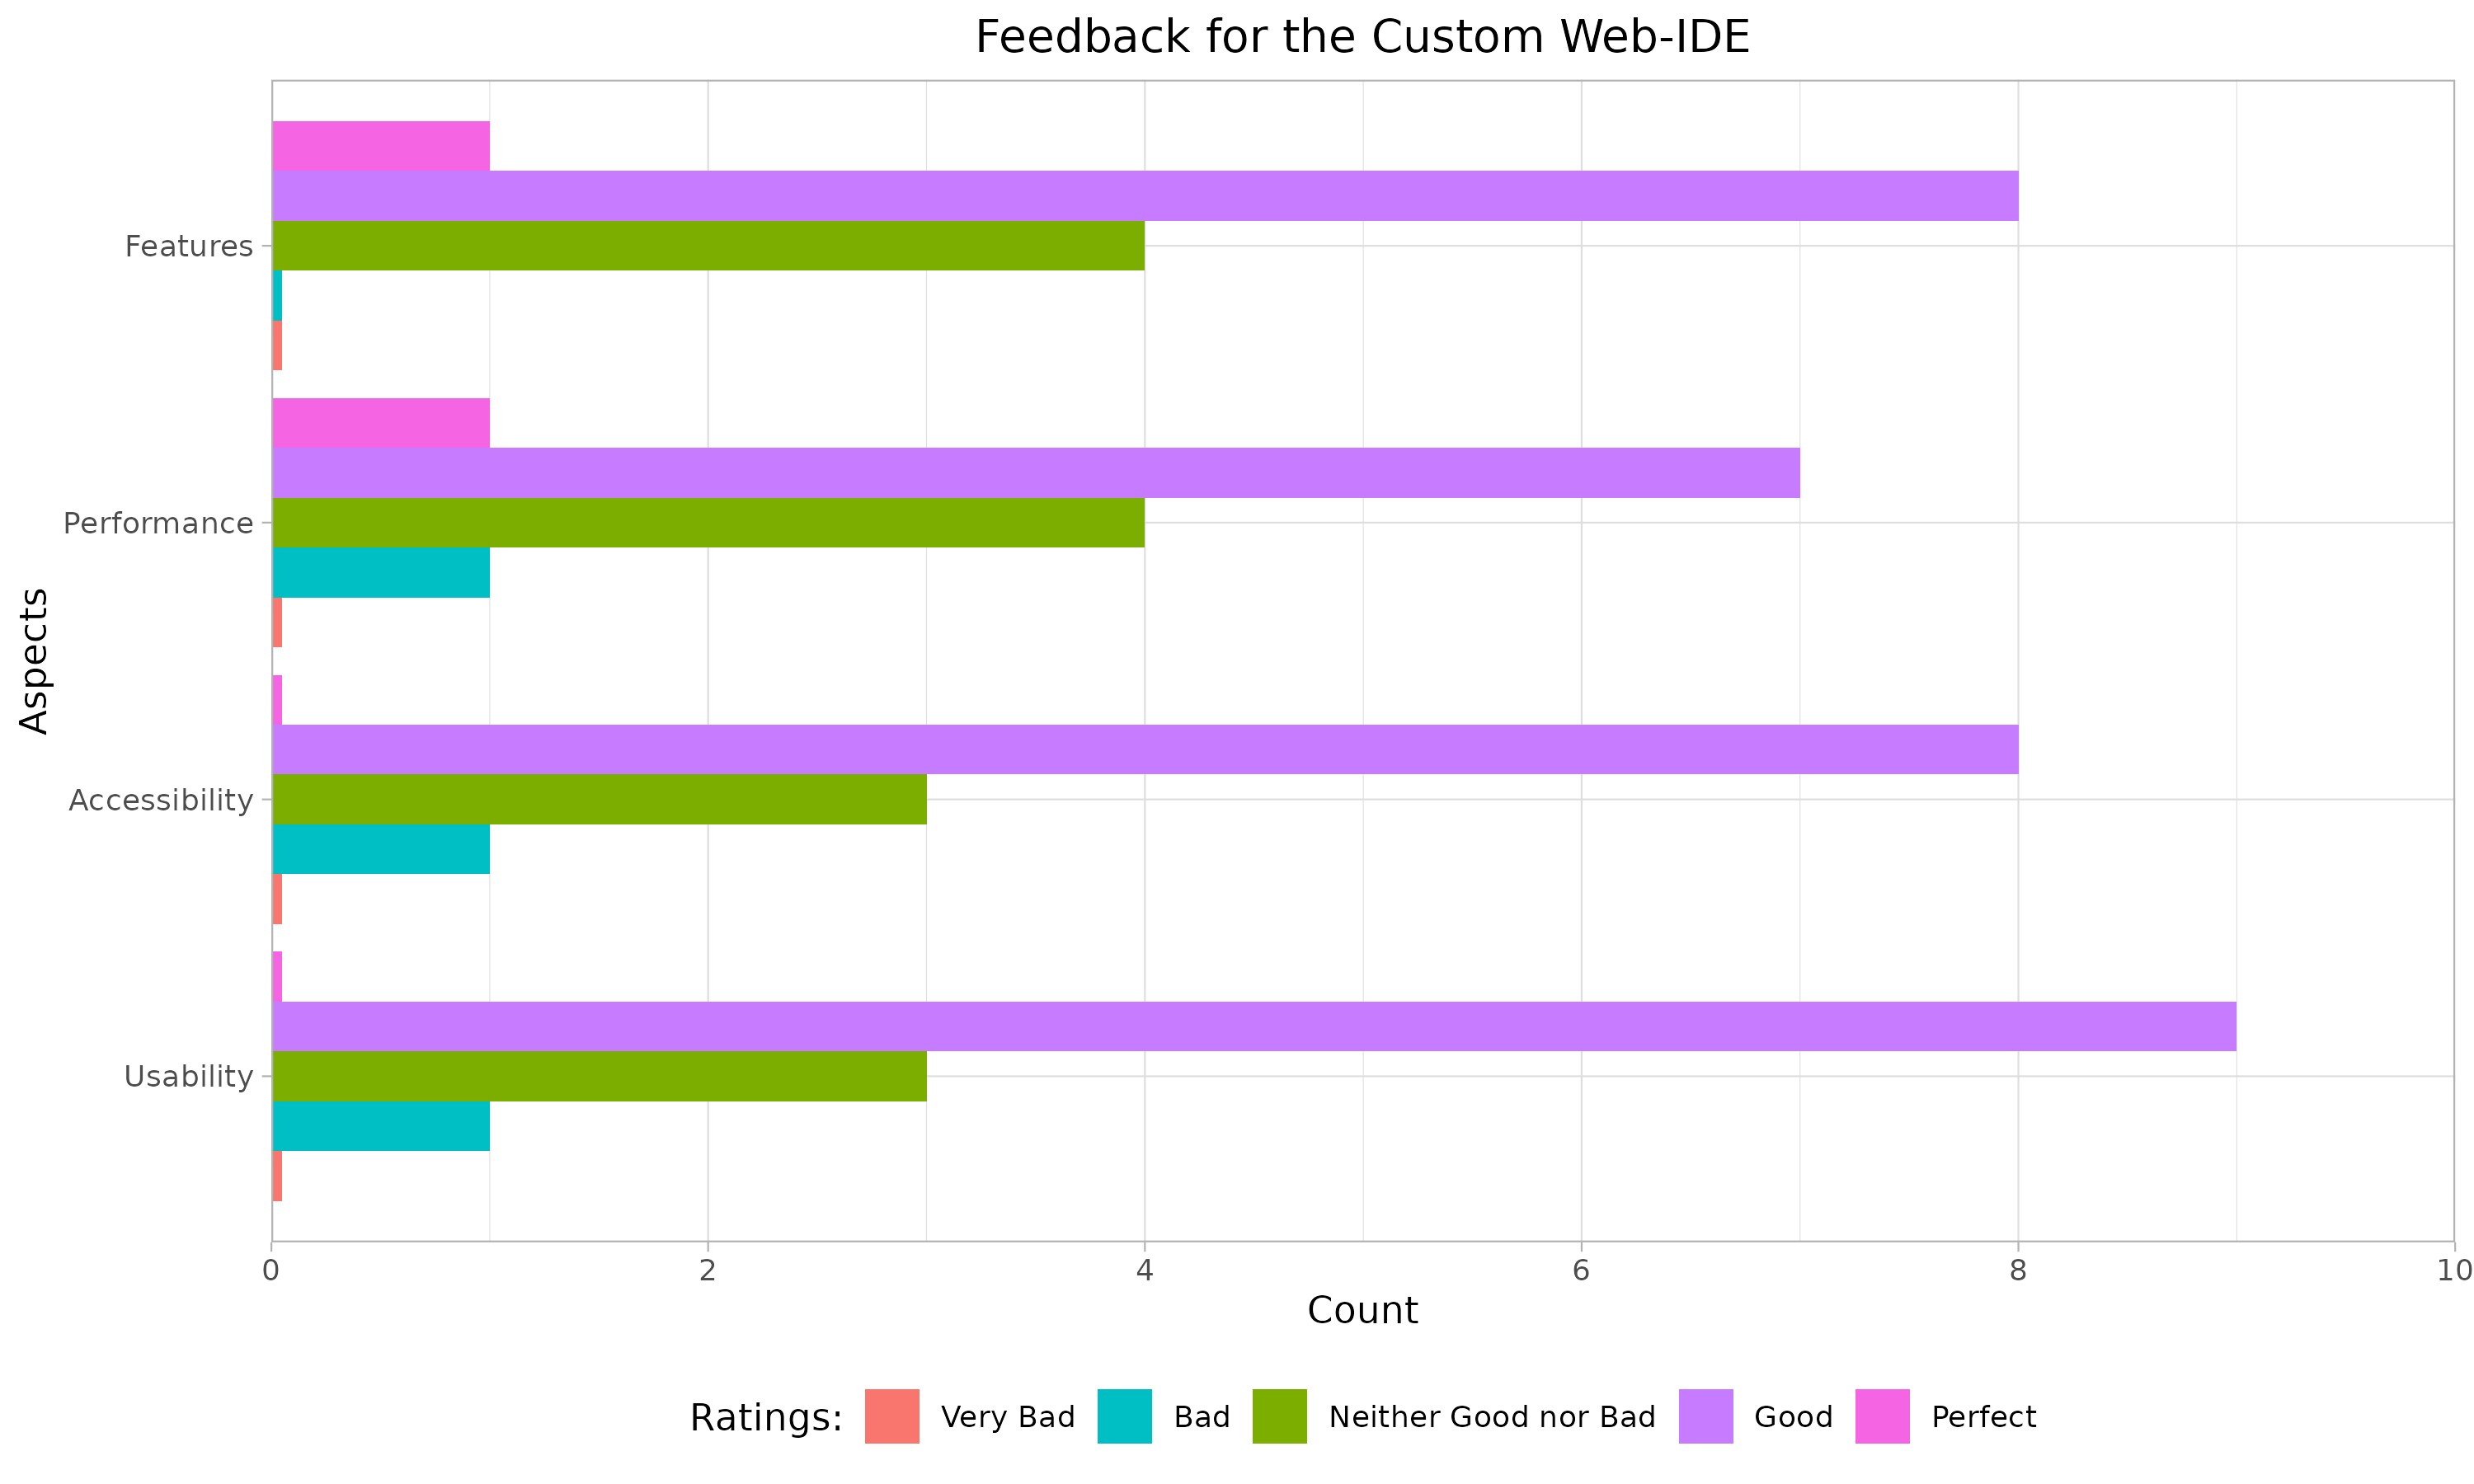
\includegraphics[width=.75\linewidth]{rstudio/survey/plots/ide.png}
    \vspace{\ftspace}
    \caption{Hackathon 2: Custom Web-IDE ratings}
    \vspace{\ftspace}
    \label{fig:website}
\end{figure}

\subsubsection{\label{sec:res_ai_code}AI Code Assistant}
In an effort to facilitate development with the Networking Library and the Smart System Platform more accessible, a LLM was primed with the code library, example code and the provided guides, as outlined in Section \ref{sec:methods_codeai}. However, the primed LLM was not directly tested and no structured feedback was gathered from users using it. Consequently, the presented feedback is of an anecdotal nature. While the LLM has been primed with knowledge of the Smart System Platform, all of its libraries, sample code and other files, including the Networking Library for networking, and mostly returns correct structure, nomenclature and commands, students reported mistakes being made in the example syntax and structure for certain commands provided by the assistant, which significantly limits the usefulness as users likely to use the AI Code Assistant are not familiar with the code and as such may not notice the incorrect code and the support provided to them.

\subsubsection{\label{sec:res_nmmct}Network Management and Module Configuration Tool}

\begin{figure}[H]
    \centering
    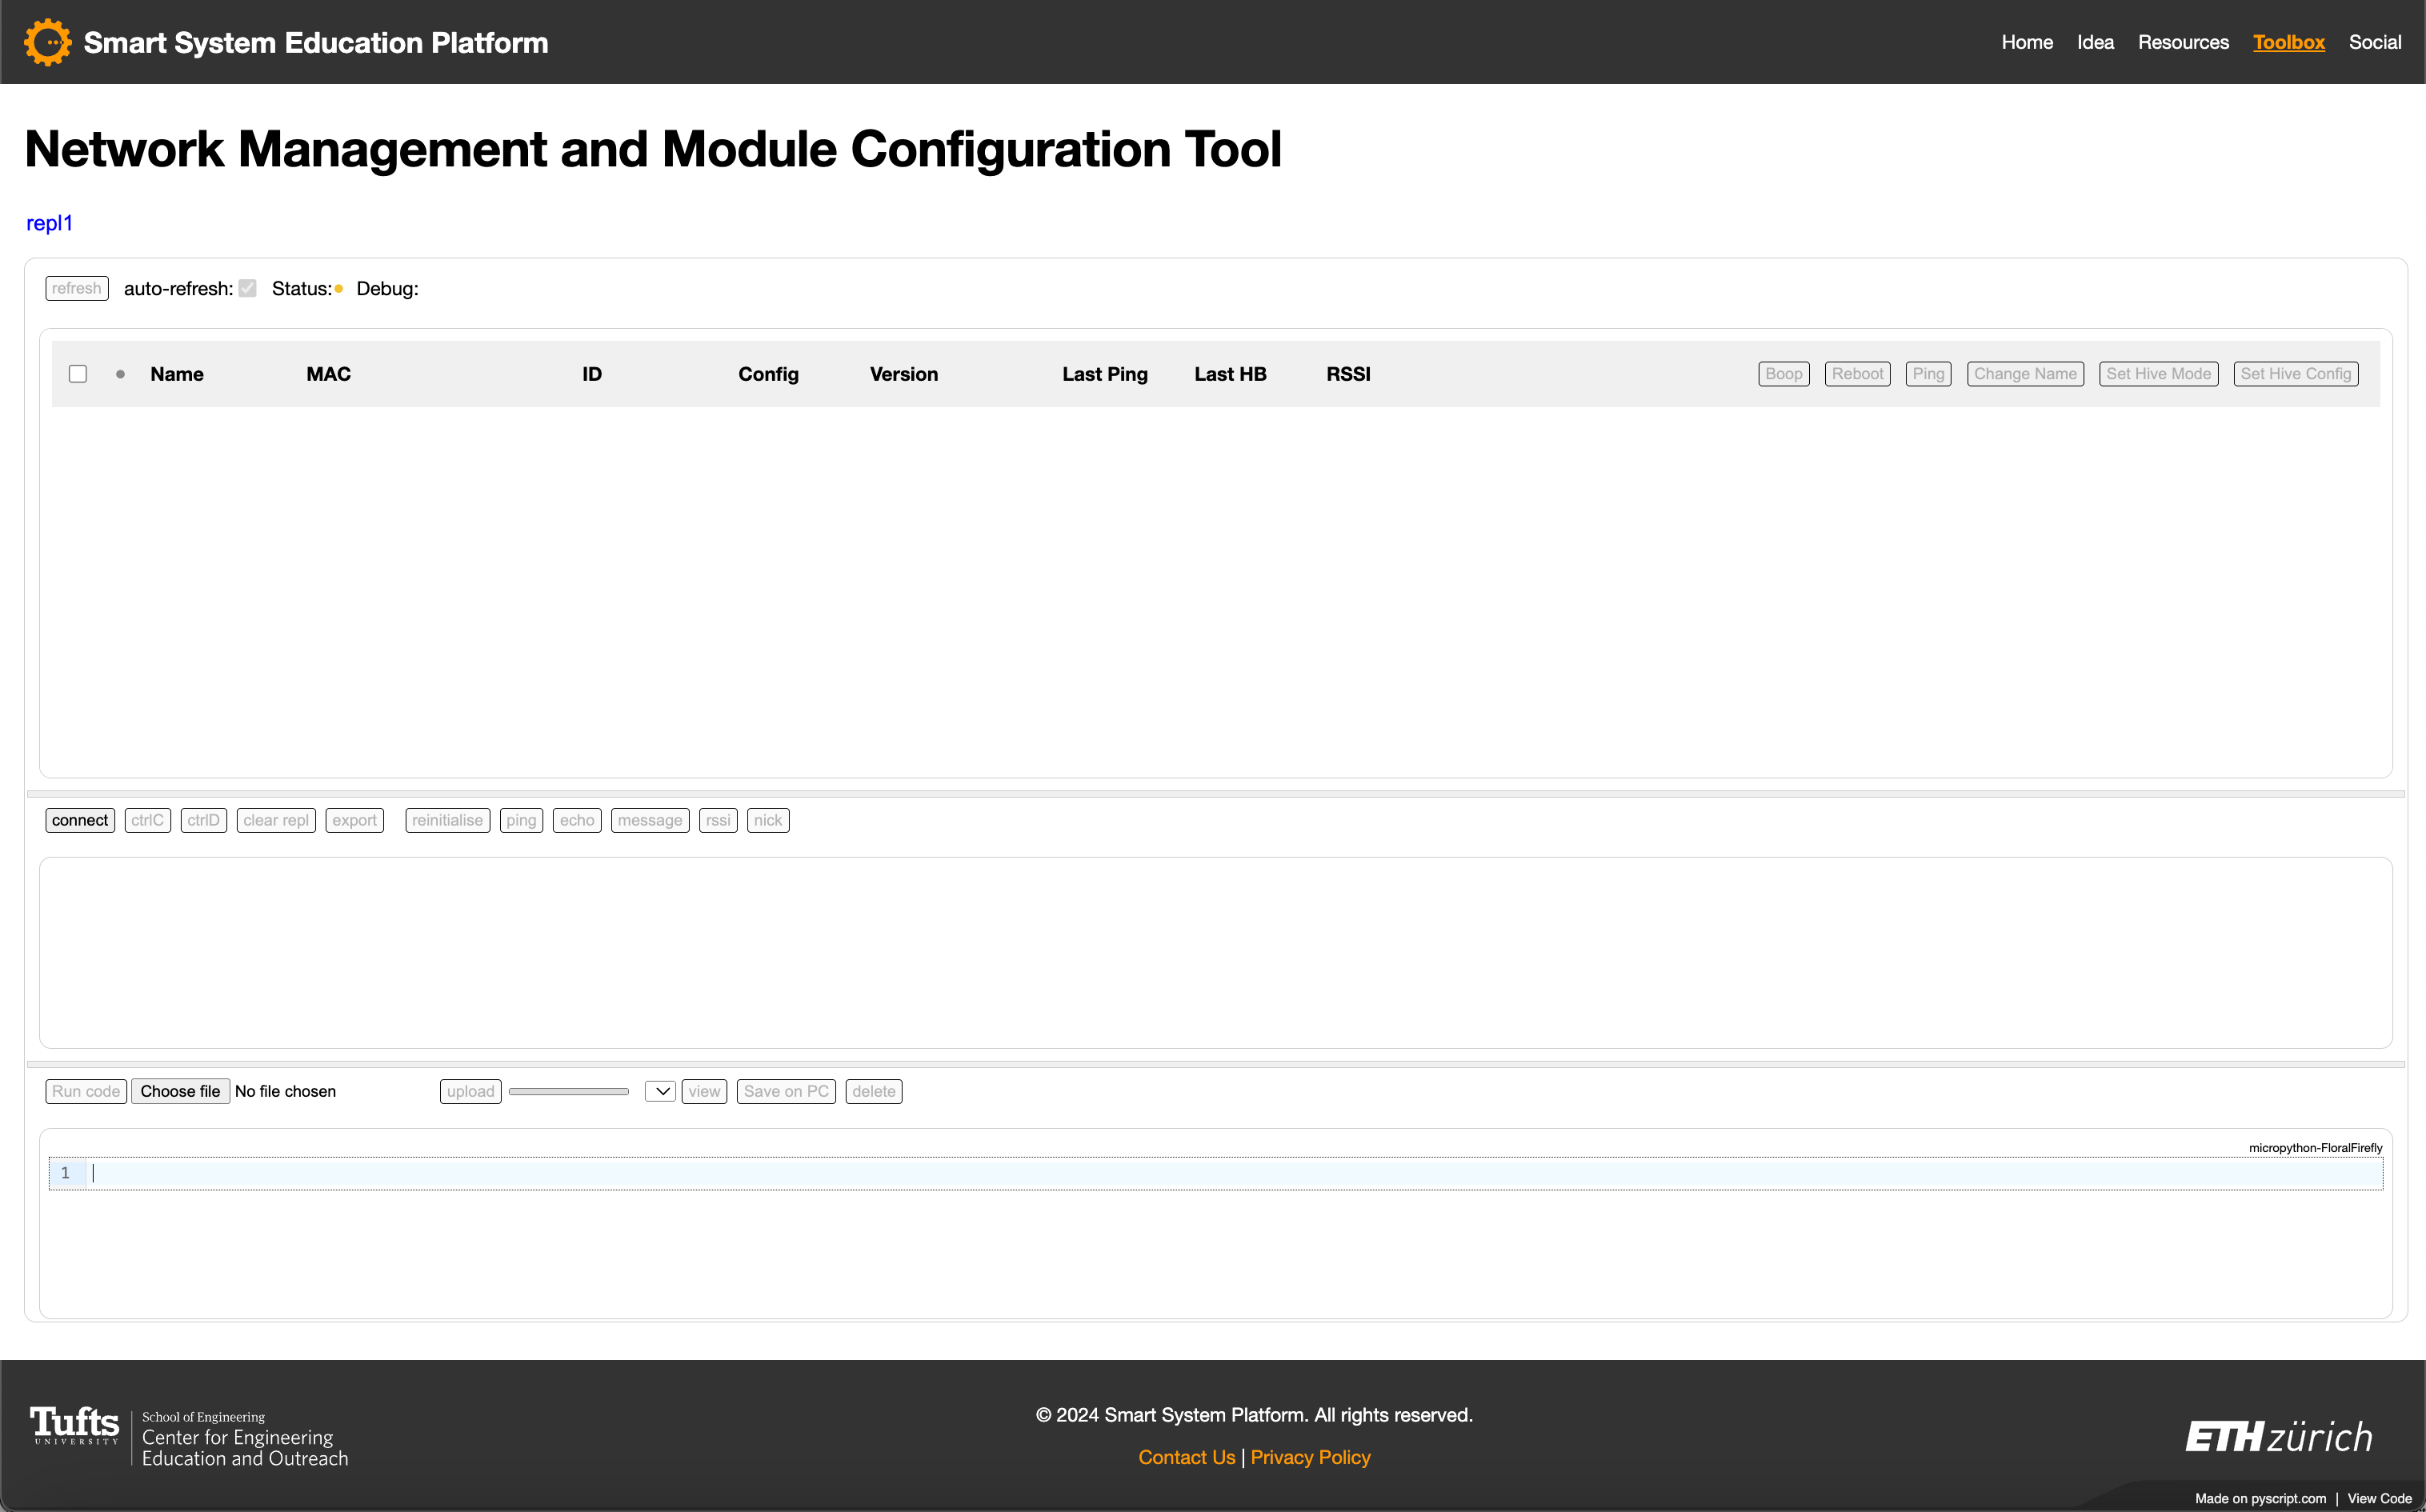
\includegraphics[width=\linewidth]{overleaf/images/nmmct_raw.png}
    \vspace{\ftspace}
    \caption{Network Management and Module Configuration Tool}
    \vspace{\ftspace}
    \label{fig:nmmct_raw}
\end{figure}

The Network Management and Module Configuration Tool has been developed to allow and facilitate management of the networking operations and associated modules using the Networking Library. The tool hence has a number of features, which include the ability to find any Smart Module with an initialised network class, retrieve information from the module such as name, configuration and more, and to send commands to the module directly from the web page. The web page has also been designed to work with the hive mode program written for some sample modules, which allows modules to be configured to send their data to specific MAC addresses, and to use data sent from specific other modules in a specific way. Further details and more in-depth discussion of that program and functionality can be found in Section \ref{sec:res_examplekit}.

\begin{figure}[H]
    \centering
    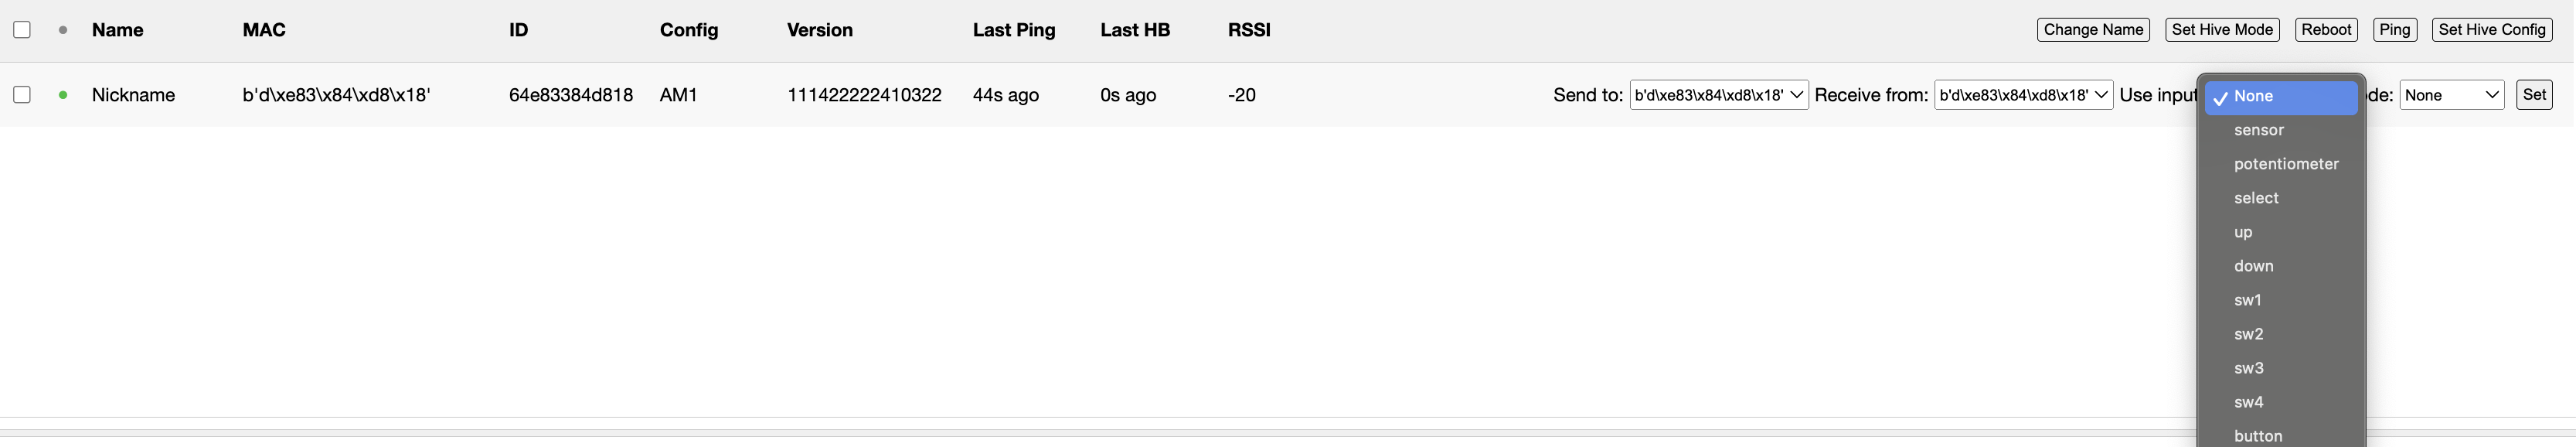
\includegraphics[width=\linewidth]{overleaf/images/nmmct_drop2.png}
    \vspace{\ftspace}
    \caption{Network Management and Module Configuration Tool: Drop-down configuration feature with input options}
    \vspace{\ftspace}
    \label{fig:nmmct_drop}
\end{figure}

In order to further simplify the use of the Network Management and Module Configuration Tool in connection with the \textit{hive mode} program, drop-down based configuration had been developed, which is shown in Figure \ref{fig:nmmct_drop}. Instead of the arduous task of manually inputting the variables into the command prompt, the configuration command can be sent with the press of a button, using the values set via the drop-down menus, which are populated with the information of all the other operational modules found in the vicinity. This feature is a result of feedback gathered during the hackathons and was subsequently developed and not tested in the hackathons. \\

This webpage incorporates all the necessary technical capabilities and could serve as the back-end for a graphical user interface (GUI). A notable limitation of the tool is that ESP-NOW-based networking can not be accessed directly from a computer or a website, necessitating the connection of a Smart Module with an initialised network library to the computer via USB to serve as a gateway.

\begin{figure}[H]
    \centering
    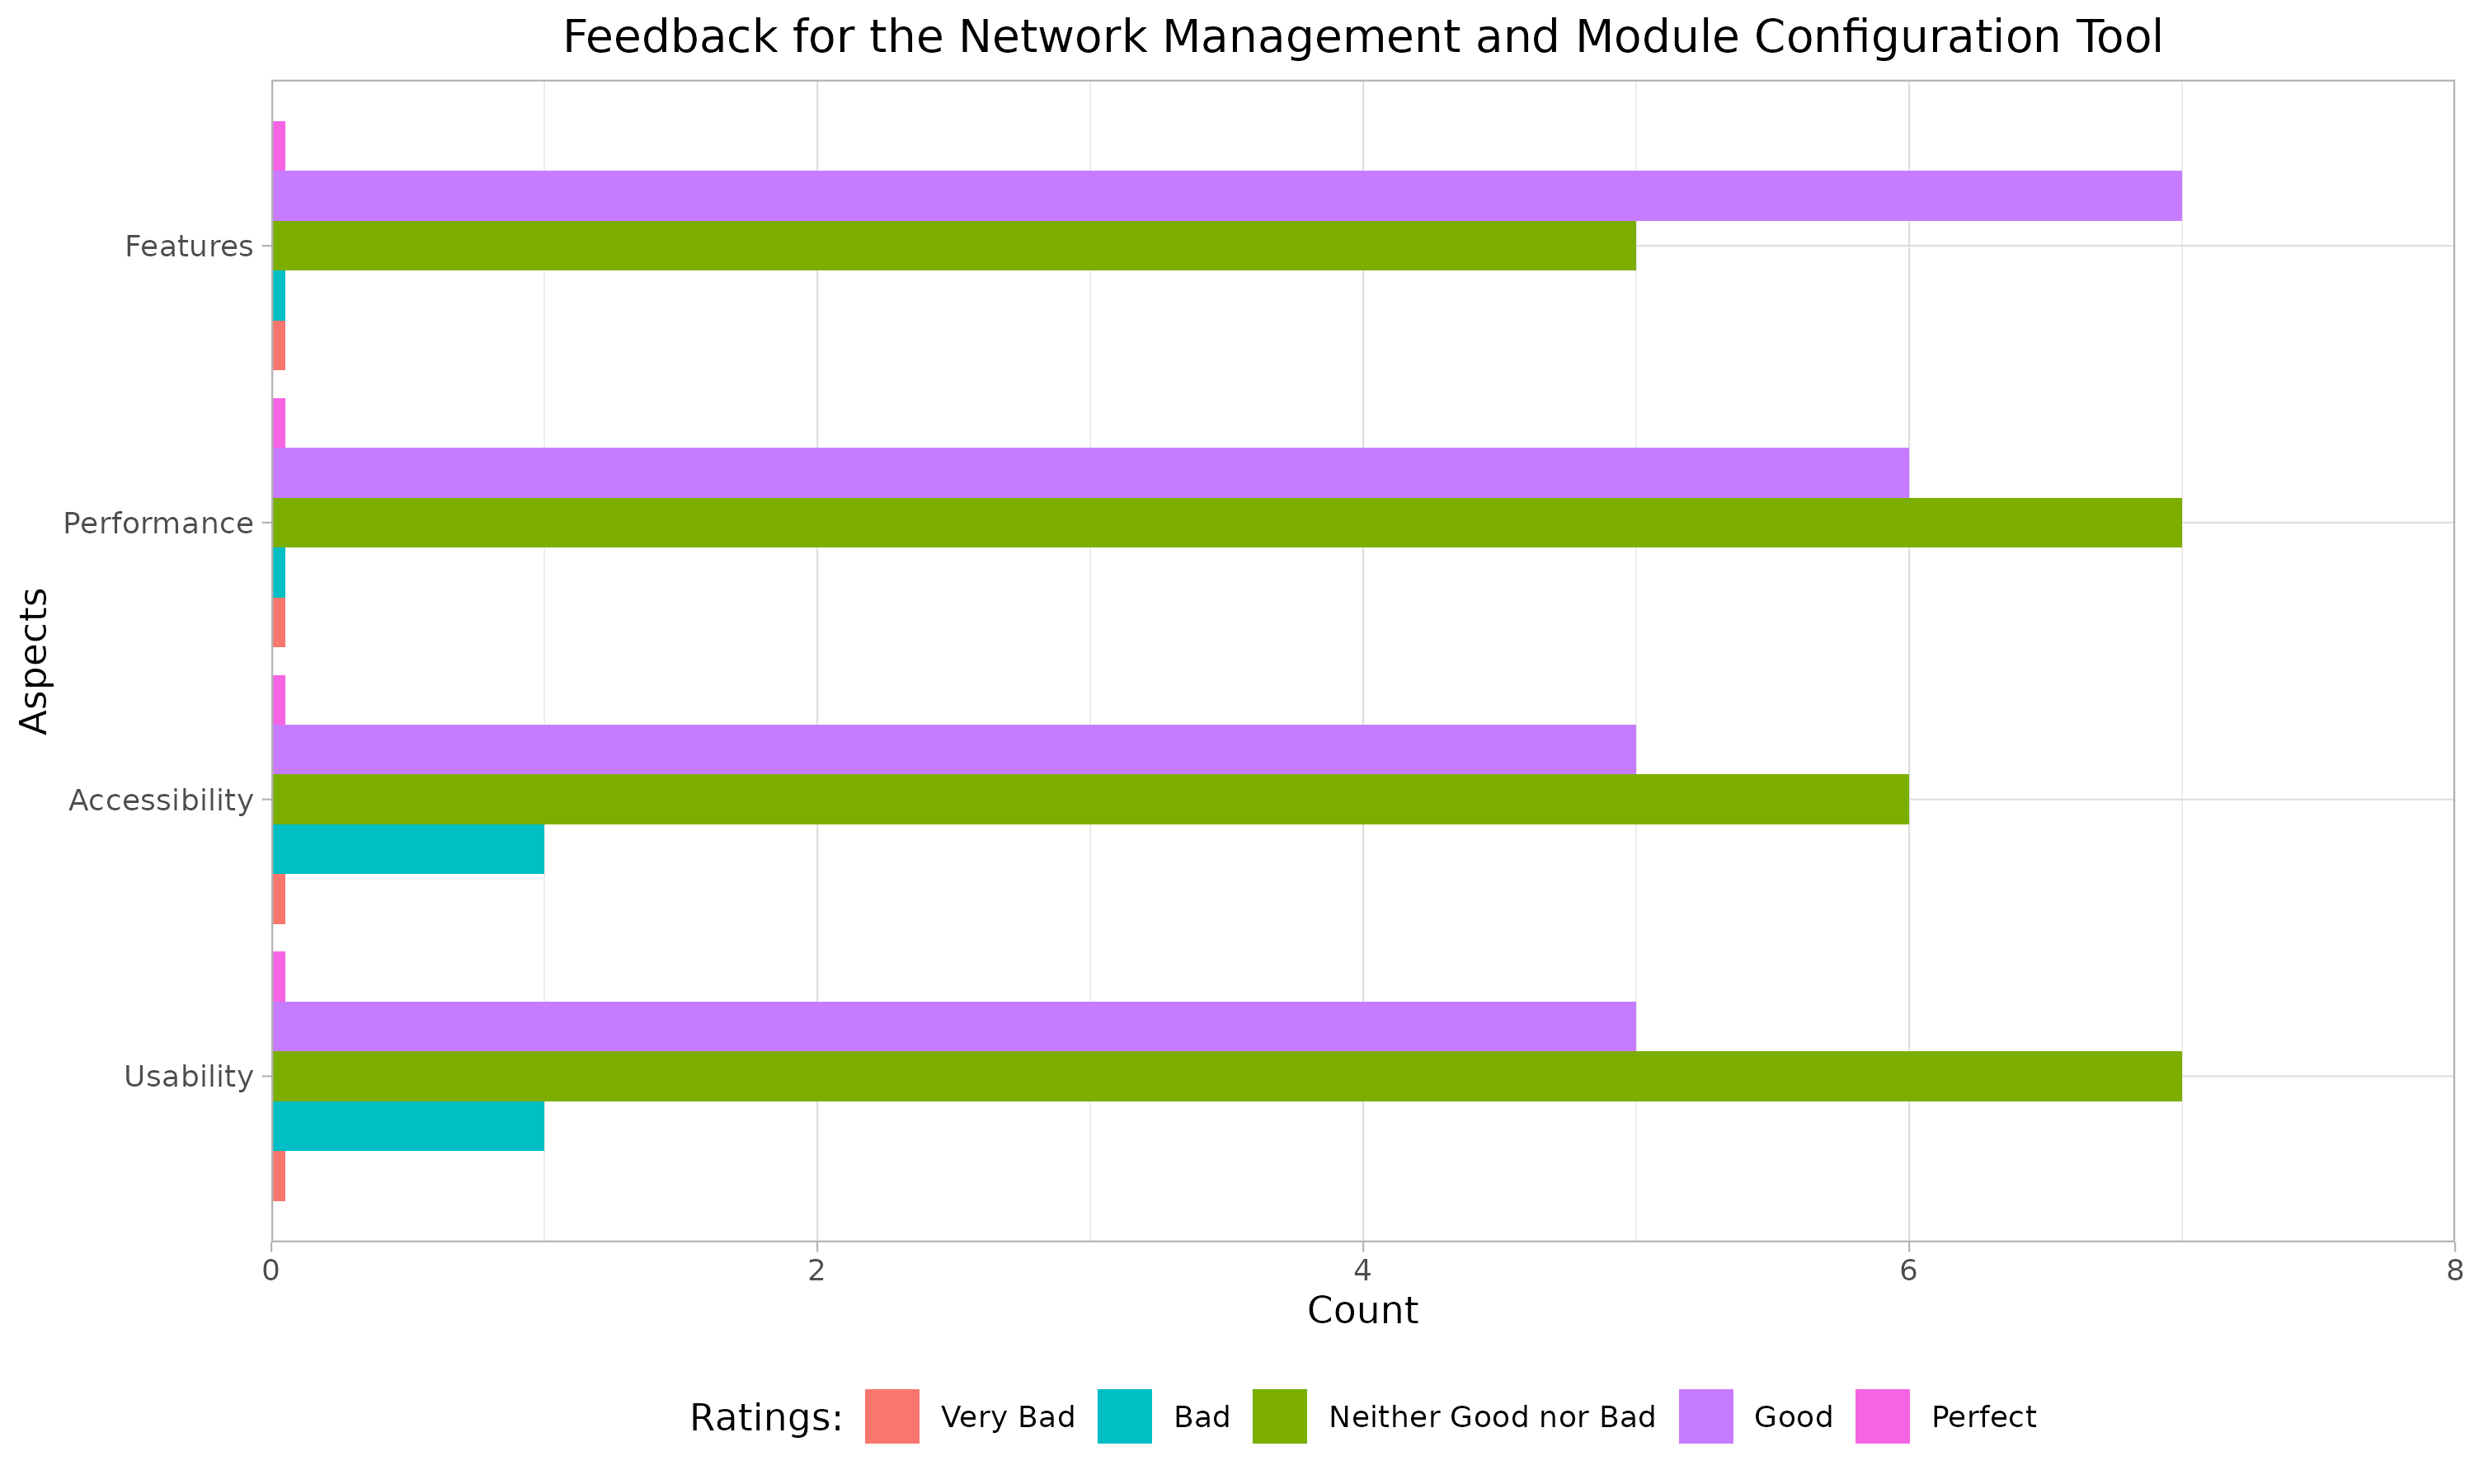
\includegraphics[width=.49\linewidth]{rstudio/survey/plots/nmmct.png}
    \vspace{\ftspace}
    \caption{Hackathon 2: Network Management and Module Configuration Tool ratings}
    \vspace{\ftspace}
    \label{fig:nmmct_q}
\end{figure}

Based on the evaluation gathered in Hackathon 2, shown in Figure \ref{fig:nmmct_q}, the ratings for this tool are mediocre in all areas, with only the features receiving a slightly positive rating. Despite the existence of a user guide provided on the website, it appears that the tool was too complex and not intuitive enough to be considered accessible. This assertion is supported by the participants' comments. Although the tool had all the necessary features and capabilities in terms of functionality and technology, the complexity of the GUI and the tool itself acted as a barrier to its usability. Users therefore found it difficult to make constructive use of the tool.

\subsubsection{\label{sec:res_ai_config}AI Module Configuration Assistant}

As outlined in Section \ref{sec:methods_configai}, an additional LLM was primed to assist in the hive configuration to make modules interact. However, while the tool was useful in principle, when it worked and provided accurate information, similar to the problems encountered with the AI Code Assistant, this LLM also exhibited issues with the accuracy of the output it provided. Specifically, the LLM was expected to provide the necessary configuration values for the configuration fields, however, it frequently parsed the provided data incorrectly. For example, it confused  the MAC address of the MCB with the chip ID, returning the latter instead of the MAC address for the required values for the hive configuration command. In these cases the usefulness of this tool was diminished significantly.

\subsubsection{\label{sec:res_mmt}Module Management Tool}

As described in Section \ref{sec:methods_up}, this tool has been developed to facilitate updating the software of a Smart Module. This is achieved by checking the version number in the configuration file of the motor against the latest release version to determine if an update is required. Based on the selected configuration, the latest software files are downloaded from the \textit{software/release} folder of the Smart System Platform GitHub and loaded onto the module, updating the \textit{config.py} file accordingly. This process is automated, thereby minimising the need for user intervention.

% \begin{figure}[H]
%     \centering
%     
\includegraphics[width=0.5\linewidth]{overleaf/images/placeholder.png}
%     \vspace{\ftspace}
%     \caption{Module Management Tool}
%     \vspace{\ftspace}
%     \label{fig:mmt}
% \end{figure}

% \subsection{\label{sec:res_hardware}Hardware}

% Module approach

% Future board

% Smart Playground

% etc.

% in Figure \ref{fig:met_hardware}.

%\subsection{\label{sec:res_software}Software}

\section{\label{sec:res_validation}Utilisation and Outcomes}

%This section presents the findings on how the Networking Library, Smart System Platform, and associated tools were utilised. In addition to some 

%To assess their effectiveness and gather user feedback, two hackathons were conducted at the CEEO FETLab, providing valuable insights into their practical applications and usability.

%In an effort to test and gather feedback on the developed networking capability, the Smart System Platform and the developed tools, two hackathons were conducted at the CEEO FETLab.

\subsection{\label{sec:res_examplekit}Example Applications}
%ehhhhhhhhh, maybe present the three little programs I had written here

In the course of the research for this thesis, a number of example programs were developed, a selection of which is introduced and described here: 
\begin{itemize}
    \item \textbf{boop-o-meter:}\\
    The boop-o-meeter program was developed during the early stages of the Networking Library's development, with the objective to evaluate and demonstrate the direct peer-to-peer and peer-to-all messaging capabilities of the ESP-NOW-based networking approach. The program runs on a Dahal board, and makes use of the included user interface in the form of the screen to display information and buttons for interaction. In addition, it includes the capability to scan for nearby devices, which will sends out a \textit{ping} command to the broadcast address. Based on the \textit{pong} returned by other devices in the vicinity, a list of the discovered devices' MAC address, in addition to the general broadcast MAC address, is populated and displayed on the screen. By selecting one of the entries a message is sent to the selected recipient. The program tracks the number of sent and received messages, with a maximum set at 999 for each.
    \item \textbf{Hive Motors:}\\
    In order to demonstrate the networking capabilities of Smart Motors, a showcase was prepared in which two Smart Motors were hard-coded to transmit their sensor data streams to each other using the developed Networking Library. Rather than using their own sensor input to be mapped against the output for the standard Smart Motor program, they use the other Smart Motor's sensor, thereby transforming the program into a collaborative task, with each motor exerting control over the other. This configuration was adopted to demonstrate the data transmission capabilities of the networking approach.
    \item \textbf{Hive Mode Program:}\\
    In an effort to facilitate interaction of different Smart Modules without the necessity of manually hardcoding, an approach was devised to allow configuration of the module interaction using networking commands. The software has been adapted to run a \textit{boot.py} file, which determines the configuration based on the entry in \textit{config.py} and runs the corresponding main program. This program initialises the networking and other required libraries and then, by default, runs the main stand-alone logic of the module, if available. For example, in the case of Smart Motors, the aforementioned \textit{boot.py} initialises the SSP Add-on Library, which in turn initialises the Networking Library, and checks if the module is in hive mode, and if it is not, runs the main stand-alone Smart Motor program. However, with the networking initialised, the module becomes discoverable, and is able receive messages and commands, and can be managed by the Network Management and Module Configuration Tool. The second part of the name of the tools derives from the ability to send configuration commands to the respective modules, a functionality that has been added for this specific mode of operation. Upon receiving a hive configuration command, the module saves the transmitted configuration values into the configuration file. This configuration consists of the MAC addresses of the modules to which it should send its data, the MAC addresses of the module it should expect data from and which sensor data should be used to determine the output, the rate at which messages should be sent, and the mode of interaction. The module then reboots and enters hive mode, in which it operates according to its hive configuration. The concept is illustrated in the Figure \ref{fig:hivemode}.
\end{itemize}

\begin{figure}[H]
    \centering
    \begin{subfigure}{0.3\textwidth} 
        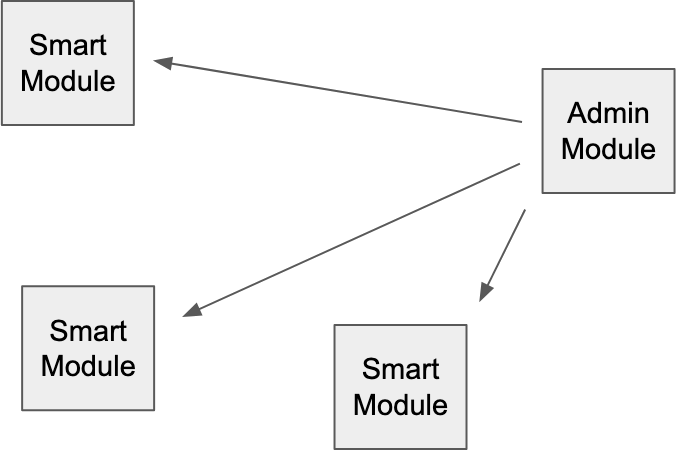
\includegraphics[width=.8\linewidth]{overleaf/images/hive1.png}
        \caption{Admin module sends command with configuration to set modules into hive mode}
    \end{subfigure}
    \hspace{10pt}
    \begin{subfigure}{0.3\textwidth} 
        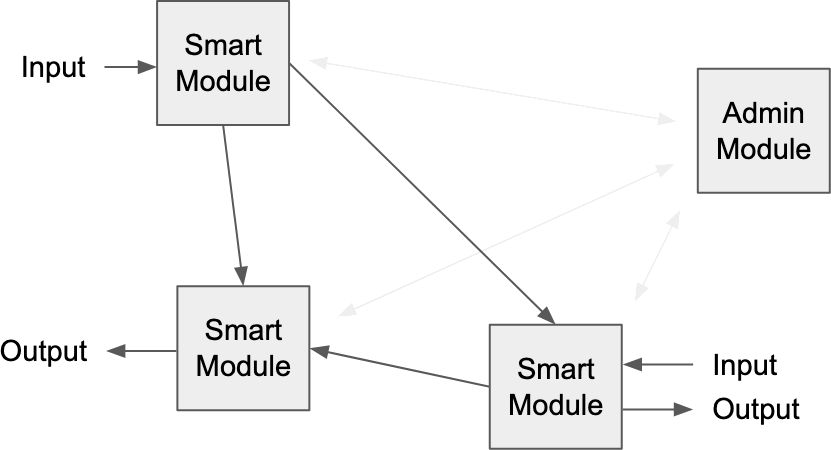
\includegraphics[width=\linewidth]{overleaf/images/hive2.png}
        \caption{Modules in hive mode sending, receiving and processing the data as configured}
    \end{subfigure}
    \hspace{10pt}
    \begin{subfigure}{0.32\textwidth}
        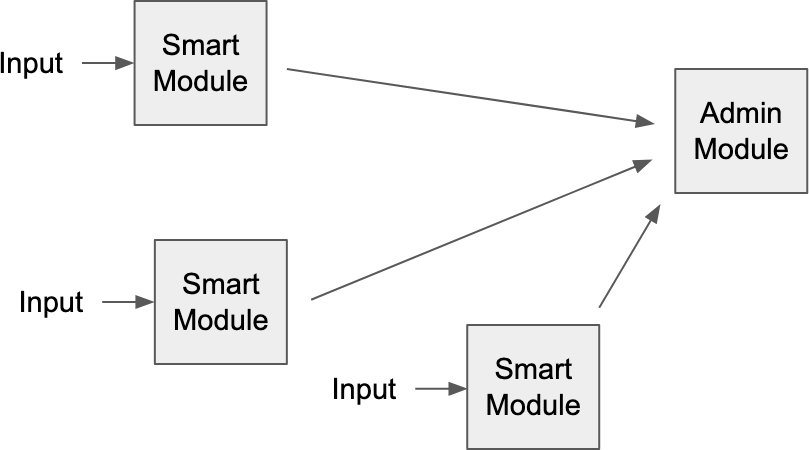
\includegraphics[width=\linewidth]{overleaf/images/hive3.png}
        \caption{Alternatively, the modules can be set up to send all of their sensor data to the Admin Module}
    \end{subfigure}
    % \begin{subfigure}{0.45\textwidth} 
    %     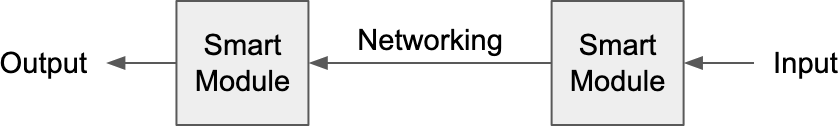
\includegraphics[width=\linewidth]{overleaf/images/hive0.png}
    % \end{subfigure}
    \vspace{\ftspace}
    \caption{Hive mode operation illustrations}
    \vspace{\ftspace}
    \label{fig:hivemode}
\end{figure}

\subsection{\label{sec:res_hackathon1}Hackathon 1}

The first hackathon was designed to evaluate the Networking Library and gather ideas for potential applications. It also involved conducting the reliability test using the \textit{boop-o-meter} program, the result of which are discussed in Section \ref{sec:res_reliability}. While users demonstrated engagement with both the Networking Library and the concept of the Smart System Platform, the feedback from participants revealed significant challenges in getting started with the library, particularly for those with no prior coding experience. The absence of structured onboarding materials rendered the initial setup difficult, and the provided \textit{example.py} file was insufficient as a starting point. Groups encountered issues with fundamental tasks, such as trying to find their MAC address. Additionally, the high volume of network messages, due to every participant broadcasting to all others on the same channel, resulted in confusion and made meaningful project development challenging. Furthermore, a majority of IDEs used by the groups, it was only possible to connect and code one module at a time, which rendered the development of networking applications, which required coding on both the sender and the recipient side challenging when only using a single computer.\\

These insights underscored the need for improved onboarding support, including structured documentation, enhanced example code, and development tools to streamline accessibility and flatten the learning curve. Consequently, these results have directly led to the development of the various development and management tools with the aim of improving accessibility, which were introduced and used during Hackathon 2.\\

During the ideation phase, teams generated a broad array of creative concepts, ranging from rudimentary communication tools to more complex interactive experiences. Some basic ideas included sending messages, smiley faces, custom images, and poking interactions between modules. Others explored game-based applications, such as hide and seek, tag, and a silent assassin-style game, where the modules used RSSI to help players locate their targets. More advanced concepts emerged as well, such as \textit{Boop Among Us}, a game inspired by social deduction mechanics, as well as virtual data ball throwing and catching, which utilises accelerometer data. Teams also proposed practical and educational applications, including mesh data logging for school science curricula, wireless collaborative reward/punishment-based training using networking, and a collaborative, sensor-driven navigation game. These ideas showcase the versatility of the Networking Library and its potential for playful, collaborative and educational use. Nonetheless, the majority of the proposed applications were linear in nature, with few proposals where behaviour and interaction depended on multiple interconnected Smart Modules.

\subsection{\label{sec:res_hackathon2}Hackathon 2}

During the second hackathon, teams were again challenged to brainstorm ideas and develop functional prototypes using the Networking Library and the SSP development tools. The primary objective of this activity was to observe what the participants would come up with, and to ascertain the efficacy of the tools in enabling the rapid design and development of networked prototypes. The focus remained on exploring the potential of the Smart System Platform to facilitate efficient development and experimentation, enabling teams to build and iterate on their projects with minimal setup time.\\

The teams proposed a variety of creative ideas, including a game utilising the hive mode of Smart Modules, where motors were configured to respond to button presses, kicking a ball towards an opponent, a motor simulating a carnival ride, which could be controlled with a networked module in terms of speed, rotations, and state (on/off), as well as a motion-based red-light green-light game where a Smart Splat displayed either a red or green light, while an accelerometer sensor on another module tracked player movement, enforcing the movement or no movement phases.

\begin{figure}[H]
    \centering
    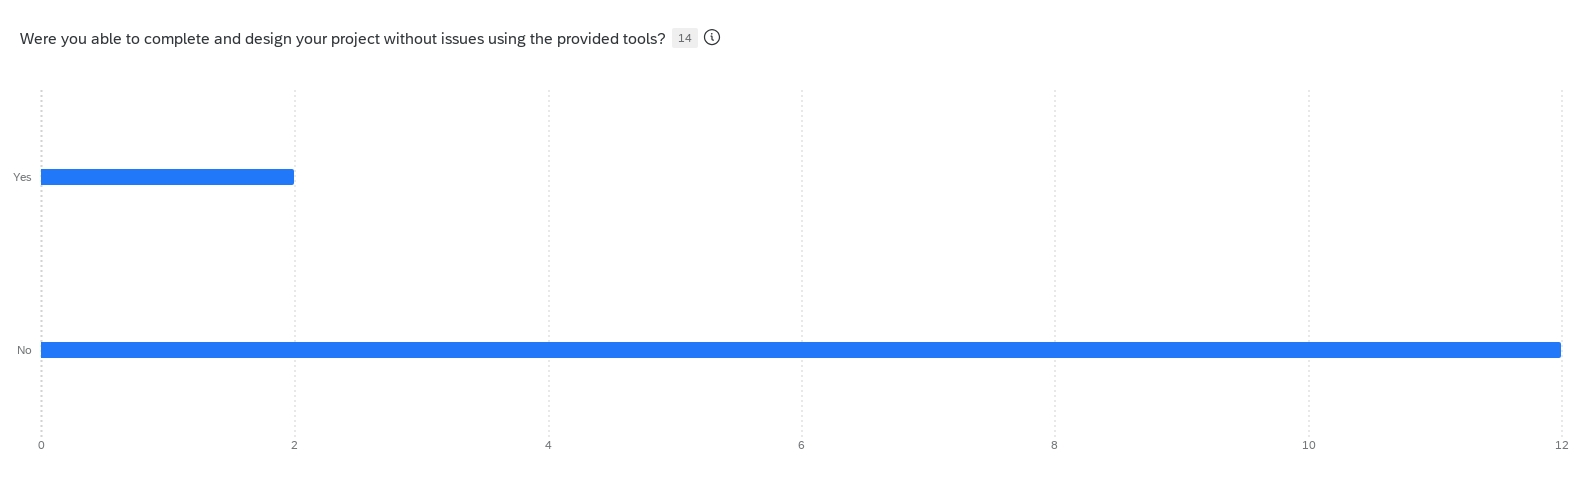
\includegraphics[width=.49\linewidth]{overleaf/images/completion.jpg}
    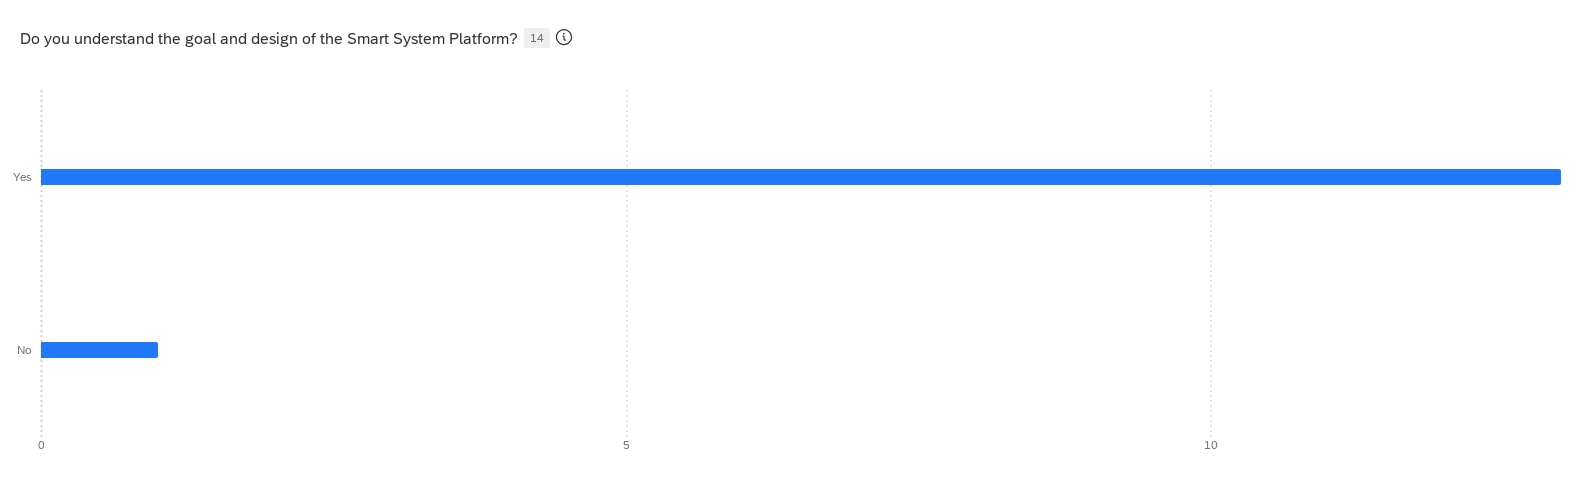
\includegraphics[width=.49\linewidth]{overleaf/images/ssp_goal.jpg}
    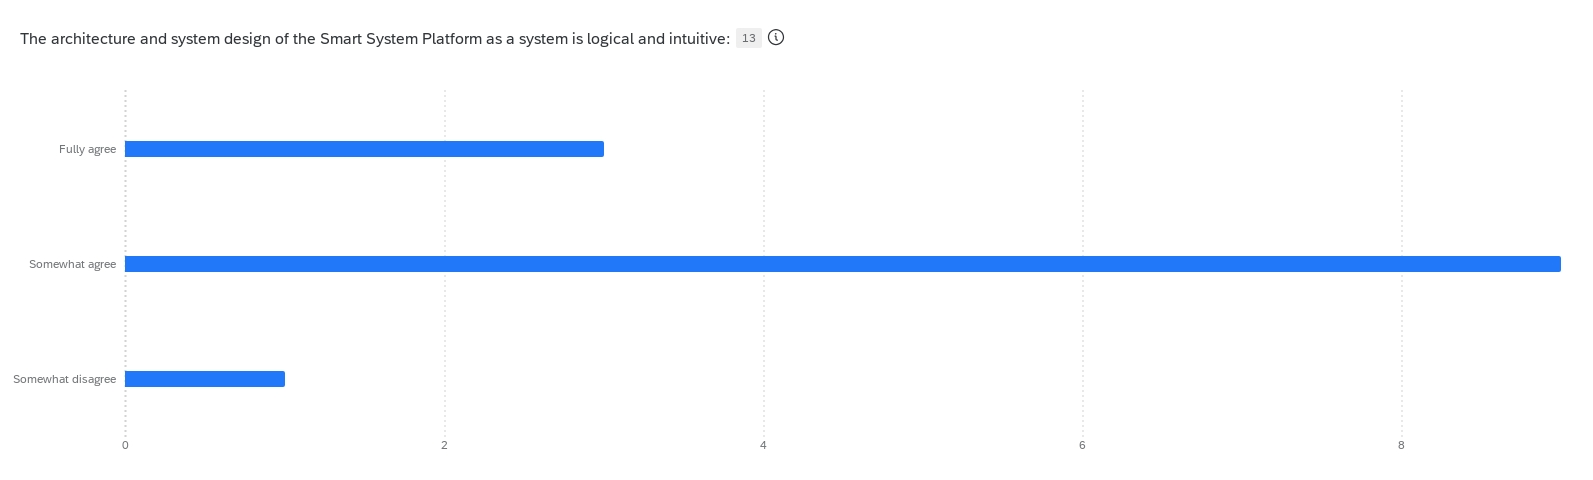
\includegraphics[width=.49\linewidth]{overleaf/images/ssp_architecture.jpg}
    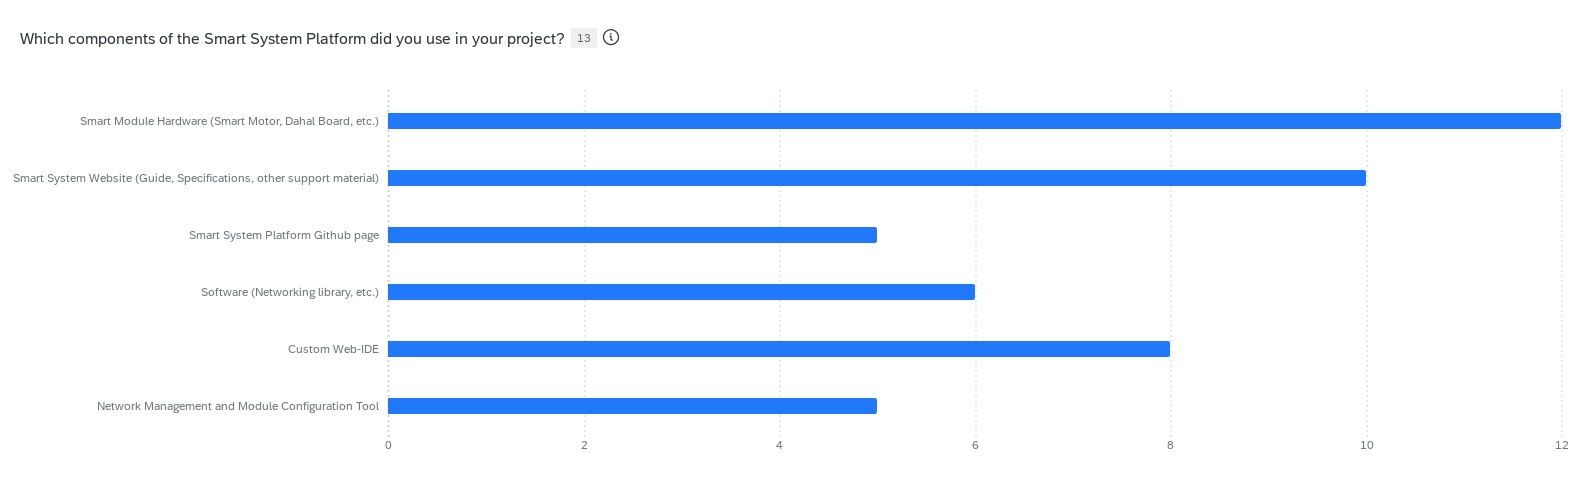
\includegraphics[width=.49\linewidth]{overleaf/images/tool_use.jpg}
    \vspace{\ftspace}
    \caption{Hackathon 2 Questionnaire results}
    \vspace{\ftspace}
    \label{fig:hack2_questions}
\end{figure}

As discussed in Section \ref{sec:res_tools}, the tools received mostly positive feedback. However, this is contrasted by the fact that a majority of teams were unable to develop a fully functional prototype during the hackathon, as shown in Figure \ref{fig:hack2_questions}. The limited time available was cited as the primary challenge, which prevented participants from completing their projects, followed by the complexity and usability of the tools provided. Conversely, the participants expressed that they understood the goal and design of the Smart System Platform, with a majority concurring that the system is both logical and intuitive. The key conclusion of the hackathon was that the entry barrier for using the provided tools was too high, especially given the limited amount of time available. Participants found the tools complex and unintuitive, making it difficult to prototype efficiently within the given time-frame. These insights highlighted the need for more user-friendly onboarding materials and an even more simplified development workflows to enhance accessibility in future iterations.

\subsection{\label{sec:res_smartplayground}\label{sec:res_honourablementions}Smart Playground}

The Smart Playground project successfully integrated the Networking Library, thereby enabling communication between various interactive modules. Some of these modules were based on the Dahal Board and the ESP32C3 MCBs, while others were custom-built and based on the ESP32C6. The various modules have been introduced in Section \ref{fig:met_hardware} and are shown in Figure \ref{fig:hardware_examples}. Two game modes were designed:
\begin{itemize}
    \item \textbf{Sequence Game:}\\
    Smart Buttons, each assigned a number and an assigned colour, are distributed across the playground area. At a central control board, one of the handheld stuffed animal modules is held in close proximity of the control board, and is assigned the coder role. The individual who is assigned this role then goes around the playground with their module, collecting a sequence. This is achieved by pressing the button on the Smart Button module, which sends out a \textit{ping} command that detects which module is closest based on the RSSI values. By pressing the button on the handheld stuffed animal module, the sequence step is added to their module. The step is represented in the form of a coloured dot on the module's LED matrix. Once a complete sequence has been collected, the coder returns to the control board, where the sequence is sent to the control board. The sequence of colours is then displayed on the control board and up to four players are then tasked to reproduce the sequence in the correct order. This is done by retracing the steps of the coder and going to the various button modules and adding the steps to their stuffed animal modules, while the control board keeps track of their progress. A player has completed the game once they have collected all the steps of the given sequence.
    \item \textbf{Music Game:}
    The music game functions in a similar manner to the sequence game. However, in lieu of Smart Buttons distributed around locations, the Smart Splats are kept in a central location and are assigned a sound and colour. The user can then collect these sounds on their modules by stomping on the Smart Splats. Once the notes have been collected, they can then send them to the control board, which in turn will play the sequence of notes collected.
\end{itemize}

%\begin{figure}[H]
%    \centering
%    \includegraphics[width=0.5\linewidth]{}
%    \caption{Caption}
%    \label{fig:smartplayground}
%\end{figure}

The interaction and wireless communication, as well as proximity detection based on RSSI, are both facilitated by the Smart System Platform Networking Library. In addition, all the developed hardware is compatible and in line with the concept of the Smart System Platform. The collaboration between Tufts CEEO and Boston University highlights the potential for real-world educational applications using the networking capabilities and tools of the Smart System Platform.\\

While the system successfully fulfilled the communication and networking requirements of that project, feedback and observations during use highlighted areas for further refinement. In particular, user feedback from various applications led to targeted tests and improvements in the Networking Library and Smart System Platform throughout their development. Notably, battery performance and RSSI angle tests were directly influenced by anecdotal reports from users working with the system.

% \subsubsection{\label{sec:res_me35}ME35}

% The base networking module has been used by students for something.

% How did they like it?

% Limitation: Feedback is limited as only some students have used the library for their projects. Though from these students, feedback has been positive.

